\chapter{Tau Lepton Decay Mode Classification}
\label{chap:Tau}

\chapterquote{I once tried standing up on my toes to see far out in the distance, but I found that I could see much farther by climbing to a high place.}%
{Xun Kuang, 313 BC $-$ 238 BC}%: Blackwood's Magazine May 1830

The tau pair polarisation correlation from a boson decay can be used to determine statistically if the parent boson is a  scalar or a vector, and, for example, to differentiate a \PH boson from  a \PZ boson \cite{Bullock:1991my}. It can also be used to measure the CP (the product of charge conjugation and parity symmetries) of the Higgs, via \HiggsToTauTau decay process\cite{Berge:2015nua}.
 %The polarisation correlation of the tau pairs can be used to infer the spin of the parent boson, differentiating \HiggsToTauTau from \ZToTauTau.

\begin{comment}
\FIGURE{fig:tauTheorySpin} shows an example of  difference in distributions for the two channels.
\begin{figure}[!htbp]
\centering
% \begin{center}/\end{center} takes some additional vertical space
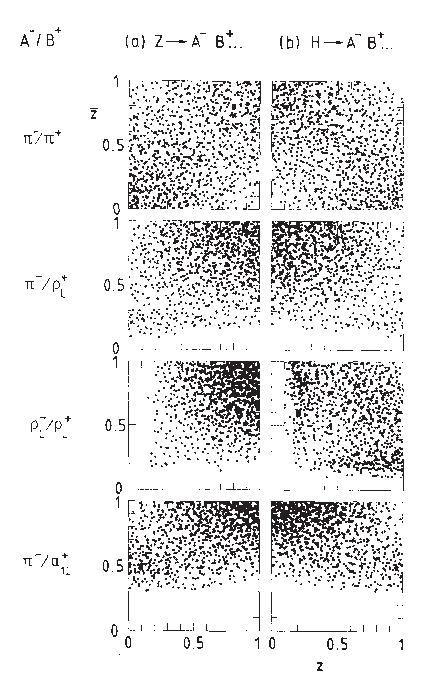
\includegraphics[width=.45\textwidth]{tau/theory}
\caption[An example of  difference in distributions for \HiggsToTauTau and \ZToTauTau.]
{
The two-dimensional distribution of (a) \HepProcess{\PZ \to \APtauon \Ptauon \to A^- B^+ \Pnut \APnut } (b) \HepProcess{\PHiggs \to \APtauon \Ptauon \to A^- B^+ \Pnut \APnut } events shown as functions of the energy fractions of $z = E_{A} / E_{\Ptauon}$ and $\overline{z} =  E_{B} / E_{\APtauon}$. In descending order the four sets of plots are for the (\APtauon, \Ptauon) pair decaying into (\Ppiminus, \Ppiplus), (\Ppiminus, $\rho_L^+$), ($\rho_L^-$, $\rho_L^+$) and finally (\Ppiminus, $a_{1L}^+$), each together with a \Pnut \APnut neutrino-pair. Plot is taken from \cite{Bullock:1991my}.
}
\label{fig:tauTheorySpin}
\end{figure}
\end{comment}

Since the tau lepton has a very short mean decay lifetime of 290\,fs \cite{Abreu:1991jn}, only tau decay products can be detected in the calorimeters and tracking detectors of the \ILD detector. Therefore, the performance of the calorimetric and tracking systems determines the ability to reconstruct tau lepton decay products and to classify different tau decay modes.

%The efficiency of tau decay mode classification can be used as a benchmark for detector performance.

The main challenge in classifying the tau lepton hadronic decay modes  is the reconstruction and  separation of spatially close photons. For  tau leptons with energies above tens of GeVs, the visible decay products are often highly boosted. Consequently electromagnetic showers from photons from \Ppizero decays often overlap in the \ECAL.  Reconstructing these photons as separate entities requires a good photon reconstruction. Hence the photon reconstruction algorithms described in \Chapter{chap:Photon} are used in this study. This chapter presents a study of the classification of tau decay modes in a highly granular linear collider detector.

% and a fine \ECAL spatial resolution
%Since the main difference in the topologies between some final states, for example \decayRhoFinalState and \decayAiPhoton final states,  is the number of photons from \Ppizero in the final state, the ability to reconstruct the photon pairs from \Ppizero as separate particles is crucial to differentiate tau decay modes.




%Many final states of the tau decay involves \Ppizero, where \HepProcess{\Ppizero \to \Pphoton \Pphoton}.

%This chapter is organised as follows. Firstly, the choice of samples for the analysis will be discussed. The tau decay modes of interests are identified. The pre-selection cuts and variables used in the MVA classification are then discussed. The performance of the tau decay mode classification will be given, followed by an \ECAL optimisation study using the developed tau decay mode classification. Lastly, the  tau decay mode classification is further used in a proof-of-principle analysis to demonstrate the ability to identify Higgs boson from \PZ  boson using the tau pair decay channel.

%
%The impact of the \ECAL transverse spatial resolution on the tau decay classification is demonstrated as well.



\begin{comment}
\section{Overview of the chapter}

The analysis starts with defining samples in \Section{sec:tauDecayModes}. Seven major tau lepton decay modes are chosen for the tau decay mode classification. The simulation of these tau lepton decays is described in \Section{sec:tauSim}.  The reconstruction of the event, including the reconstruction of the invariant mass resonance for \decayRho and \decayAi decay modes, is discussed in \Section{sec:tauReco}.  After defining discriminative variables used in the MVA classification in \Section{sec:tauVar}, the classification is performed with a multivariate classifier. Since the decay products of a tau lepton need to be classified into one of the seven decay modes, a multiple class classification, presented in \Section{sec:tauMVA}, is used to allow simultaneous classification between  multiple decay modes. Afterwards, the performance of the classification is described in \Section{sec:tauClassificationEff}.

%Pre-selection of the events, discussed in \Section{sec:tauPreSel}, are such that events affected by the reconstruction and detector effects, which do not vary with the \ECAL cell sizes, are taken out of this analysis.

The classification of the tau lepton decay modes is used for the \ECAL optimisation study. The impact of  the \ECAL cell sizes,  as well as the tau lepton energy,  on the classification performance is studied in \Section{sec:tauECAL}.

The tau decay mode classification is then utilised in \Section{sec:tauHZ} to demonstrate the ability to separate Higgs boson from \PZ  boson using the tau pair decay channel, where both tau leptons subsequently decay   via  \tauToPion mode.

% for different energies of tau lepton decay to access the impact of the tau energy on the classification. The classification is also used to study the impact of the \ECAL cell sizes on the classification performance,  discussed in \Section{sec:tauECAL}.

% The difference in the spin of the boson reflects in the different spin correlation of the tau pair. By extracting the spin correlation, parent bosons can be separated.
%This classification is repeated for different energies of tau lepton decay to access the impact of energy on classification. The impact of the \ECAL design is studied afterwards, where the \ECAL square cell size is varied. An overall tau hadronic decay classification efficiency is constructed to allow direct and easy comparison between different detector design and different energies of the tau decay.

% The study of the tau final state classification in the context for the  \ECAL optimisation allows the analysis to discard reconstruction and detector issue that do not vary with the \ECAL design. For example, the early photon conversion that happens in the tracking detector would complicate the event topology. But since it is affected by the tracker design, it can be ignored in this analysis. \SECTION{sec:tauSim}  and \Section{sec:tauPreSel} discuss the pre-selection cuts to choose the signal samples and events for this analysis.

%The classification is performed with a multivariate classifier. Discriminating variables are calculated before feeding into the classifier.  A \multiclass classification is used to allow simultaneous classification between  multiple final states, described in \Section{}.


%A proof-of-principle analysis to demonstrate the ability to identify \PHiggs from \PZ using  tau pair decay channel is presented in the \Section{}. The difference in the spin of the boson reflects in the different spin correlation of the tau pair. By extracting the spin correlation, parent bosons can be separated.

%The follow sections on the analysis use the a 50\,GeV tau lepton decaying sample, reconstructed with nominal the \ILD detector model.
\end{comment}

\section{Event generation and simulation}
\label{sec:tauDecayModes}

%\section{Select single tau decay}  in a \ee collider for an electron-positron collider The studied tau lepton decay channel is \eeToTauTau, with a centre-of-mass energy of 100\,GeV.   predominant effect of the tau lepton decays,

Two million \eeToTauTau events at a centre-of-mass energy of 100\,GeV were generated with  \WHIZARD \cite{whizard}.  \TAUOLA \cite{Jadach:1993hs} was used to describe the tau lepton decays with correct spin correlations of the tau decay products. The study was focused on separating tau decay modes. Hence beam effects, such as the initial state radiation and the beam induced background, were not included. The \eeToTauTau events were simulated using the \ILD detector model as described in \Chapter{chap:Reconstruction}.




\section{Event reconstruction}
\label{sec:tauReco}

Events were reconstructed with  \ilcsoft version v01-17-07 \cite{Gaede:82475} and \pandora version 3 \cite{Marshall:2015rfa}, using the photon reconstruction algorithms described in \Chapter{chap:Photon}. An event display of \eeToTauTau interaction reconstructed in the \ILD detector is shown in \Figure{fig:tauEvtDsp}. The top half of the event shows a tau lepton decaying into \decayRhoFinalState. The bottom half of the event shows a tau lepton decaying into \decayThreePionPhoton.


%As the study is aimed for optimisation study of the \ECAL cell sizes, t

\begin{figure}[!tbph]
\centering
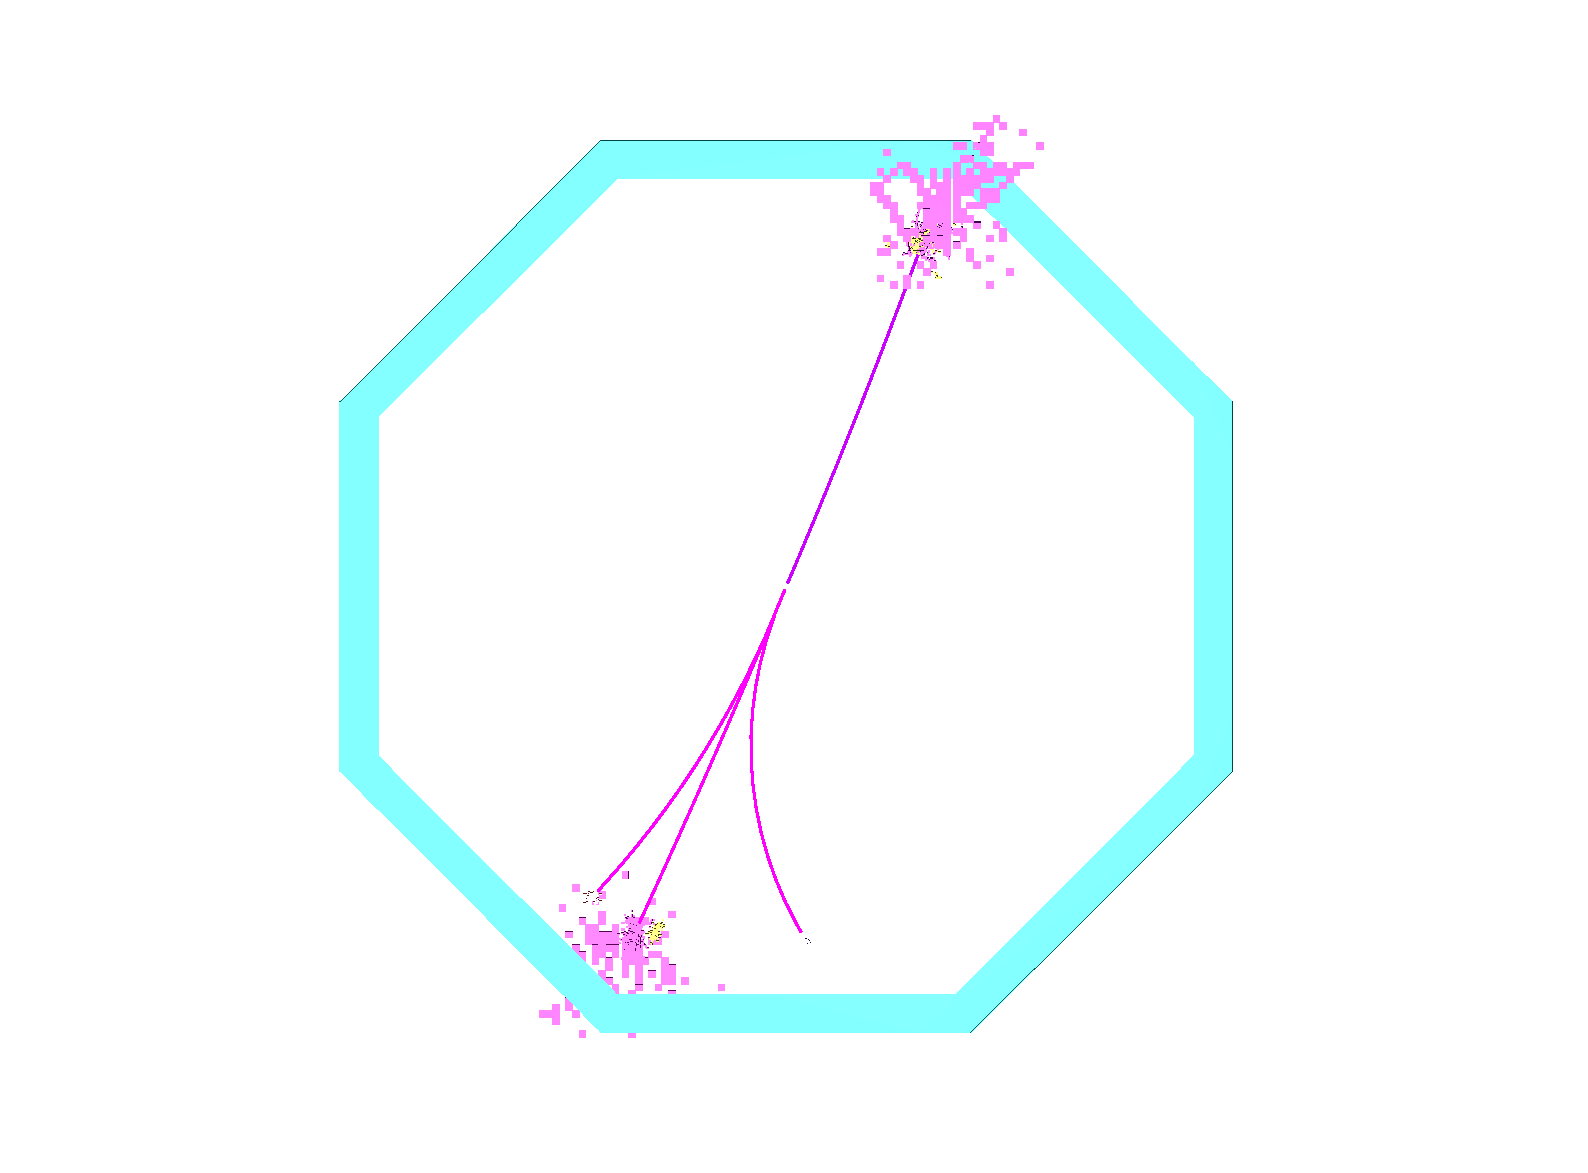
\includegraphics[width=0.7\textwidth]{tau/tau_evt_dsp3}
\caption{ An event display of a simulated \eeToTauTau event using the \ILD detector model. The top half of the event shows a tau lepton decaying into \decayRhoFinalState. The bottom half of the event shows a tau lepton decaying into \decayThreePionPhoton. Purple lines represent \Ppipm tracks in the tracking detectors. Purple squares represent  calorimeter hits of the \Ppipm hadronic showers in the \ECAL and the \HCAL. Yellow squares represent calorimeter hits of EM showers of photons  from \HepProcess{\Ppizero \to \Pphoton \Pphoton}. The blue region is the transverse cross section of the \ECAL barrel part.}
\label{fig:tauEvtDsp}
\end{figure}




\subsection{Tau  decay modes}

To study the main decay modes of the tau lepton, decay modes with branching ratios above 2\% are classified, which results in seven decay modes, covering 92.58\,\% of the tau decay branching fraction \cite{Agashe:2014kda}. The seven tau decay modes, their branching ratios, and detectable final states are listed in \Table{tab:TauDecayMode}.


In the  \decayRho decay mode, the \Prho meson subsequently decays into  \decayRhoFinalStateShort. In the \decayAi  neutral and charged decay modes, the \Pai meson subsequently decays into \decayAiPhotonFinalStateShort, and \decayAiPionFinalStateShort, respectively. The invariant masses of the \Prho meson and \Pai meson are \uprightMath{775.11\pm0.34}\,MeV and \uprightMath{1230\pm40}\,MeV, respectively \cite{Agashe:2014kda}.

%Thrust axis is useful to separate each jet in a back-to-back two-jet event.
%Thrust value, $T$, is 1 for a perfect pencillike back-to-back two-jet event, and 0.5 for a perfect spherical event. The thrust value is useful in picking out back-to-back two-jet event.


%\subsection{Tau lepton decay modes}

%Tau lepton decays into a number of final states.
% The most difficult final states to separate are \decayRhoFinalStateShort and \decayAiPhotonFinalStateShort, where photons from boosted \Ppizero are very challenging to reconstruct correctly.

\begin{table}[htbp]\centering
\smallskip
\begin{tabular}{l l r}
\hline
\hline
Decay mode  & Detectable final state & Branching ratio\\
\hline
\decayElectron   &  \decayElectronShort  & $17.83{\pm0.04\%}$   \\
\decayMuon &	\decayMuonShort & $17.41{\pm0.04\%}$  \\
\decayPion  &   \decayPionShort	& $10.83{\pm0.06\%}$   \\
\decayRho   & \decayRhoFinalStateShort& $25.52{\pm0.09\%}$ \\
\decayAi neutral  & \decayAiPhotonFinalStateShort	& $9.30{\pm0.11\%}$    \\
\decayAi charged &	\decayAiPionFinalStateShort    & $8.99{\pm0.06\%}$  \\
\decayThreePionPhoton  &	\decayThreePionPhotonShort    & $2.70{\pm0.08\%}$  \\
\hline
\hline
\end{tabular}
\caption[Decay modes, detectable final state particles and branching ratios of the seven major \Pgtm decays.]
{Decay modes, detectable final state particles, and branching ratios of the seven major tau decay modes with the largest branching ratios. Values are taken from \cite{Agashe:2014kda}.}
\label{tab:TauDecayMode}
\end{table}


\subsection{Tau selection}

The simulated \eeToTauTau event contains two tau leptons. Since the tau decay mode classification is applied on a per-tau-lepton basis, the decay products of the two tau leptons in one event are divided into two sets for individual tau decay mode classification. By identifying the axis of the back-to-back taus in the event, the detector space can be separated in two hemispheres, where particles in each hemisphere correspond to the decay products of one tau lepton.

Separating reconstructed particles in an event into two sets is achieved using the principle thrust axis vector of the event, which is the axis that most particles are aligned to. The principle thrust axis vector, $\hat{t}$, is determined by maximising the thrust \cite{PhysRevLett.39.1587}, $T$:
\begin{equation}
T = \max_{\hat{t}}\!\frac{\sum_{i}\absOf{\hat{t}\!\cdot\!\vec{p_{i}}}}{\sum_{i}\absOf{\vec{p_{i}}}},
\end{equation}
where $\vec{p_{i}}$ is the momentum vector of particle $i$;  vector $\hat{t}$ is the unit principle thrust axis vector; and index $i$ is summed over all particles in an event. Two sets of particles are obtained based on the sign of the scalar product between the principle thrust axis vector  and the momentum vector of a particle; particles with a positive sign of the scalar product are in one set and particles with a negative sign of the scalar product are in another set.


\section{Pre-selection}
\label{sec:tauPreSel}


For the purpose of this study, three pre-selection cuts, based on the MC information of the particles,  are used. The cuts and the number of tau decays passing the cuts are listed in \Table{tab:tauPreSelEff}.

Since this study is focused on photon reconstruction in the \ECAL to classify tau decay modes, the tau decays with photon converting to electron pairs in the tracking detector are not considered.

The focus of the study is on higher energy tau decays. Tau decays with the total visible energy (i.e. not accounting for neutrinos) of tau decay products, $E_{vis}^{MC}$, less than 5\,GeV are not considered.



Lastly, tau decays are discarded when the tau decay products are in the gap region between barrel and  endcap parts of the calorimeters, because there is a degradation in the particle reconstruction efficiency in this region. Tau decays with the generated polar angle of the tau lepton in the region $0.6 < \absOf{\theta_{\Ptau}^{MC}} < 0.9$\,rad are not considered.

%The cut demands the absolute value of the generated polar angle of the tau lepton with respect to the beam direction, $\absOf{\theta_{Z,MC}}$, is between 0.3\,rad and 0.6\,rad to be  in the endcap region, or is between 0.8\,rad and $\frac{\pi}{2}$\,rad to be  in the barrel region.


%Simulated events are further constrained to focus on the events with clear topologies, based on the truth information. The constraints on the samples are

%Three sets of constraints are used. One set of constraints is that events are discarded when photons in the tau decay products convert to electron pairs in the tracking detector. Since the reconstruction does not attempt to recover photons from electron pairs, these events would have a fewer number of photons reconstructed than expected.


%.  Since the reconstruction does not attempt to recover photons from electron pairs, events with converted photons are discarded.

%, which changes the topologies of the final states.

%Another set of constraints requires the total energy of the non-neutrino tau decay products, $E_{vis,MC}$, to be greater than 5\,GeV. If most energy of a tau lepton is carried by  neutrinos, non-neutrino decay products would have low energies and be difficult to be reconstructed.

%Hence these events with low-energy non-neutrinos tau decay products are not used in the analysis.



%Last set of constraints requires events to be discarded when tau decay products deposit energies in the gap region between barrel and  endcap part of the calorimeter. As the reconstruction   does not attempt to recover reconstruction in the gap region, there is a degradation in the particle reconstruction efficiency in the gap region. The constraint demands the absolute value of the polar angle of tau lepton with respect to the beam direction, $\absOf{\theta_{Z,MC}}$, is between 0.3\,rad and 0.6\,rad to be  in the endcap region, or is between 0.8\,rad and $\frac{\pi}{2}$\,rad to be  in the barrel region.

\TABLE{tab:tauPreSelEff} shows the fractions of tau decays passing successive cuts  for different tau decay final states.  As expected, the cut on  photon conversions only affects tau decay modes with  photons in the final states. The cut on the total visible energy of the tau decay products has the greatest effect on the leptonic decay modes with two neutrinos  in the final states. The cut on the tau polar angle affects different tau decay modes equally.

% because more energies are carried by neutrinos in these decay modes.

%All decay modes are affected almost equally by this cut, suggested by numbers in \Table{tab:tauPreSelEff}.



\begin{table}[htbp]\centering
\smallskip
\begin{tabular}{ l r r r}
\hline
\hline
 \multicolumn{1}{L{0.2\textwidth}}{Final state}   & \multicolumn{1}{R{0.2\textwidth}}{No photon conversion} & \multicolumn{1}{R{0.2\textwidth}}{$E_{vis}^{MC}$ > 5\,GeV} &\multicolumn{1}{R{0.2\textwidth}}{$\absOf{\theta_{\Ptau}^{MC}}$} \\
\hline
\decayElectron& 100.0\% & 84.7\%& 66.2\%\\
\decayMuon &100.0\%& 85.2\%&66.7\%\\
\decayPion &100.0\%& 88.3\%&60.9\%\\
\decayRhoFinalState&77.1\%&76.9\%&61.9\%\\
\decayAiPhotonFinalState &61.3\%&61.2\%&50.5\%\\
\decayAiPionFinalState &100.0\%&100.0\%&78.0\%\\
\decayThreePionPhoton &77.0\%&77.0\%&61.8\%\\
\hline
\hline
\end{tabular}
\caption
{Fractions of tau decays passing successive pre-selection cuts  for different tau decay final states.}%All cuts are based on the truth information.
\label{tab:tauPreSelEff}
\end{table}

\begin{comment}
\section{Event simulation}
\label{sec:tauSim}


The \eeToTauTau events were simulated using the \ILD detector model. The software used for simulation is described in \Chapter{chap:Reconstruction}.

%that are not affected by the varying \ECAL cell sizes
The beam specific effects are not simulated, such as the initial state radiation and the beam induced background, as the analysis is optimised for the use of the \ECAL optimisation study.





\begin{table}[htbp]\centering
\smallskip
\begin{tabular}{l r}
\hline
\hline
Cuts & Values\\
\hline
\multicolumn{1}{L{0.4\textwidth}}{Photon conversion in the tracking detector}& No \\
\multicolumn{1}{L{0.4\textwidth}}{Total energy of non-neutrino decay products} & $E_{vis,MC} > 5\,GeV$ \\
Polar angle acceptance & \multicolumn{1}{R{0.5\textwidth}}{$0.6 > \absOf{\theta_{Z,MC}} > 0.3$ or $1.57 > \absOf{\theta_{Z,MC}} > 0.8$} \\
\hline
\hline
\end{tabular}
\caption[Pre-selection cuts for tau lepton decay final state classification.]
{Pre-selection cuts for tau lepton decay modes classification.}
\label{tab:tauPreSel}
\end{table}

\section{Event pre-selection}
\label{sec:tauPreSel}

Pre-selection cuts select events using the truth information. Since the analysis is aimed for the optimisation of the \ECAL cell sizes, these pre-selection cuts are such that effects not affected by the changing of the \ECAL cell sizes are not considered in the analysis. These cuts allow the analysis to focus on the events with clear topologies. The pre-selection cuts are listed in \Table{tab:tauPreSel}. The fraction of events passing each pre-selection cut for individual decay mode are listed in \Table{tab:tauPreSelEff}.

One of the pre-selection cuts is to demand that the tau decay products  do not have photons converted to electron pairs in the tracking detector, determined with the truth information. These discarded events would have fewer photons and more electrons than expected in the final states, which changes the topologies of the final states. Shown in \Table{tab:tauPreSelEff}, only decay modes with photons in the final states are affected by this cut, as expected.


Another pre-selection cut requires the total energy of the non-neutrino tau decay products, $E_{vis,MC}$, to be greater than 5\,GeV, based on the truth information. If most energy of a tau lepton is carried by  neutrinos, non-neutrino decay products would have low energies and be difficult to be identified. Hence these events with low-energy non-neutrinos tau decay products are not used in the analysis. Decay modes with only one non-neutrino particle in the final states are mostly affected by this cut because more energies are carried by neutrinos, indicated in \Table{tab:tauPreSelEff}.

The last pre-selection cut is to discard events with tau decay products depositing energies in the gap region between barrel and the end cap part of the calorimeter. As the reconstruction   does not attempt to recover reconstruction in the gap region, there is a significant drop in the particle reconstruction efficiency in the gap region. The cut demands the absolute value of the polar angle of tau lepton, based on the truth information, $\absOf{\theta_{Z,MC}}$, is between 0.3 and 0.6\,rad to be contained in the end cap region, or is between 0.8 and 1.57\,rad to be contained in the barrel region. All decay modes are affected almost equally by this cut, suggested by numbers in \Table{tab:tauPreSelEff}.

\end{comment}

%The no photon early conversion cuts only effective against final states with \Ppizero, as \Ppizero decays to a photon pair. For final states with one \Ppizero, about 77\% events survived. For final states with two \Ppizero, about 61\% events survived, which is roughly $0.77^2$. For the visible angle acceptance, final states with only one particle are affected the most, whilst final states with more than one particles typically have more visible energies. The polar angle acceptance efficiencies depend on the final states, as light final states are boosted and more likely in the forward region.



%An low visible energy event is discarded if the total energy of the tau lepton visible decay products is below 5\,GeV. Requirement of the tau decay in the barrel or the end cap part of the calorimeter is defined as the polar angle of the tau is $ 17.2\degree < |\theta_{Z}| < 34.4\degree$ or $ 45.8\degree < |\theta_{Z}| < 90\degree$.



\section{Multivariate classification}
\label{sec:tauVar}

The classification of different tau decays uses a MVA classifier based on twenty-seven discriminant variables, listed in \Table{tab:tauVaraibles}. The particle ID information comes from the output of the \pandora reconstruction.

%After event reconstruction,  27 discriminative variables used in the MVA  classification  are  developed and listed in \Table{tab:tauVaraibles}. The distributions of four powerful variables for different tau decay modes are shown in \Figure{fig:tauVar}.

%Having pre-selected events,  variables are carefully developed for the multivariate analysis (MVA). The full list of the variables are shown in \Table{tab:tauVaraibles}.

\begin{table}[!htbp]\centering
\begin{tabular}{lr}
\hline
\hline
Category &  Variable \\
\hline
Particle numbers  &{  ${N}_{\charge}$, ${N}_{\Pmu}$, ${N}_{\Pe}$, ${N}_{\Pgg}$,  ${N}_{\Pgpm}$} \\
Invariant masses & {$m_{vis}$, $m_{\charge}$, $m_{\neutral}$, $m_{\Pgg}$, $m_{\Pgpm}$} \\
Energy variables & { $\tilde{E}_{vis}$,  $\tilde{E}_{\charge}$, $\tilde{E}_{\Pmu}$, $\tilde{E}_{\Pe}$, $\tilde{E}_{\Pgg}$,  $\tilde{E}_{\Pgpm}$} \\
Calorimetric energy information &   { $E^{\ECAL}_{\charge} / E_{\charge}$,  $ E^{\ECAL} / E$ } \\
\decayRhoShort reconstruction &{  $m_{\Pgpz}^{\parenths{\Prho}}$, $m_{\Prho}^{reco}$} \\
\decayAiPhotonShort reconstruction & {  $m_{\Pgpz}^{(\Pai)}$, $m^{*(\Pai)}_{\Pgpz}$, $m_{\Pai}^{reco}$} \\
EM shower profile & $\delta{l}$, $t_0$, $\langle{w}\rangle$ \\
Calorimeter hit information & $\bar{E}_{hit}$, $MIP$ \\
Track information & $E/p$ \\
\hline
\hline
\end{tabular}
\caption
{Variables used in the MVA classification for the tau lepton decay mode classification.}
\label{tab:tauVaraibles}
\end{table}

\subsection{Particle number variables}

The most crucial variables for classifying tau decay modes  are the number of different types of final state particles. There are five particle number  variables used in the MVA classification: the number of charged particles (${N}_{\charge}$); the number of muons (${N}_{\Pmu}$); the number of electrons (${N}_{\Pe}$); the number of photons (${N}_{\Pgg}$); and the number of charged pions (${N}_{\Pgpm}$). Here muon and electron IDs are provided by the \pandora outputs.


%\tauToElectron, \tauToMuon, and
\FIGURE{fig:tauVarNCharge} shows  distributions of the numbers of reconstructed charged particles for different tau decay modes. Over 98\% of   \tauToPion decays have exactly one reconstructed charged particle, and approximately 95\% of \decayAiPionShort decays give exactly three reconstructed charged particles. \FIGURE{fig:tauVarNMuon} and \Figure{fig:tauVarNElectron}  show the distributions of the numbers of reconstructed muons and electrons respectively for different tau decay modes. Here 99\% of \tauToMuon decays produce exactly one reconstructed muon, and 99\% of \tauToElectron decays have one reconstructed electron. \FIGURE{fig:tauVarNPhoton} shows  distributions of the numbers of reconstructed photons  for different tau decay modes, which distinguishes hadronic tau decay final states with different numbers of \Ppizero.  Nearly 75\% of  \decayRhoShort  decays give exactly two reconstructed photons, and over 60\% of \decayAiPhotonShort decays have exactly four photons.




\begin{figure}[htbp]
\centering
% \begin{center}/\end{center} takes some additional vertical space
\begin{subfigure}[b]{0.45\textwidth}
 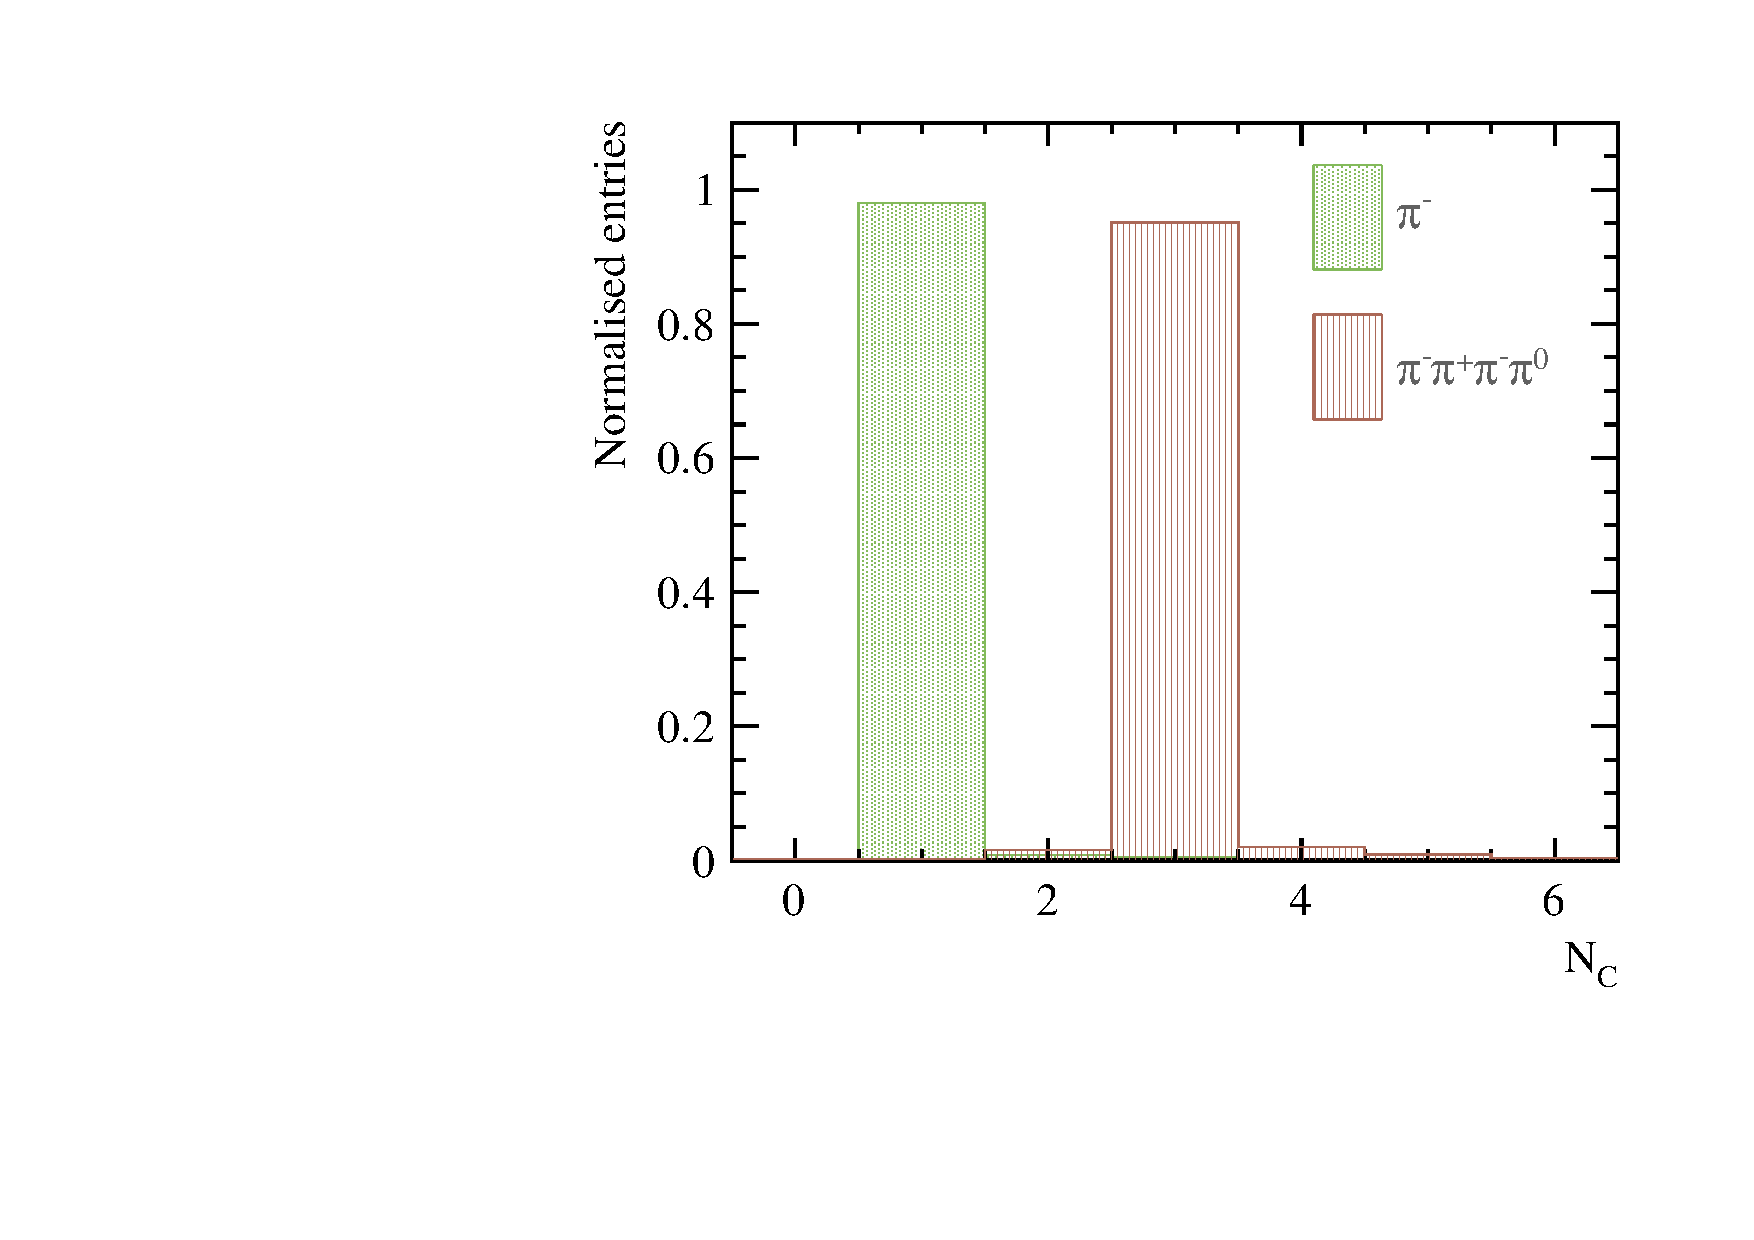
\includegraphics[width=\textwidth]{tau/var3/nCharge_100GeV_improved.pdf}
  \caption{}
  \label{fig:tauVarNCharge}
\end{subfigure}
\begin{subfigure}[b]{0.45\textwidth}
 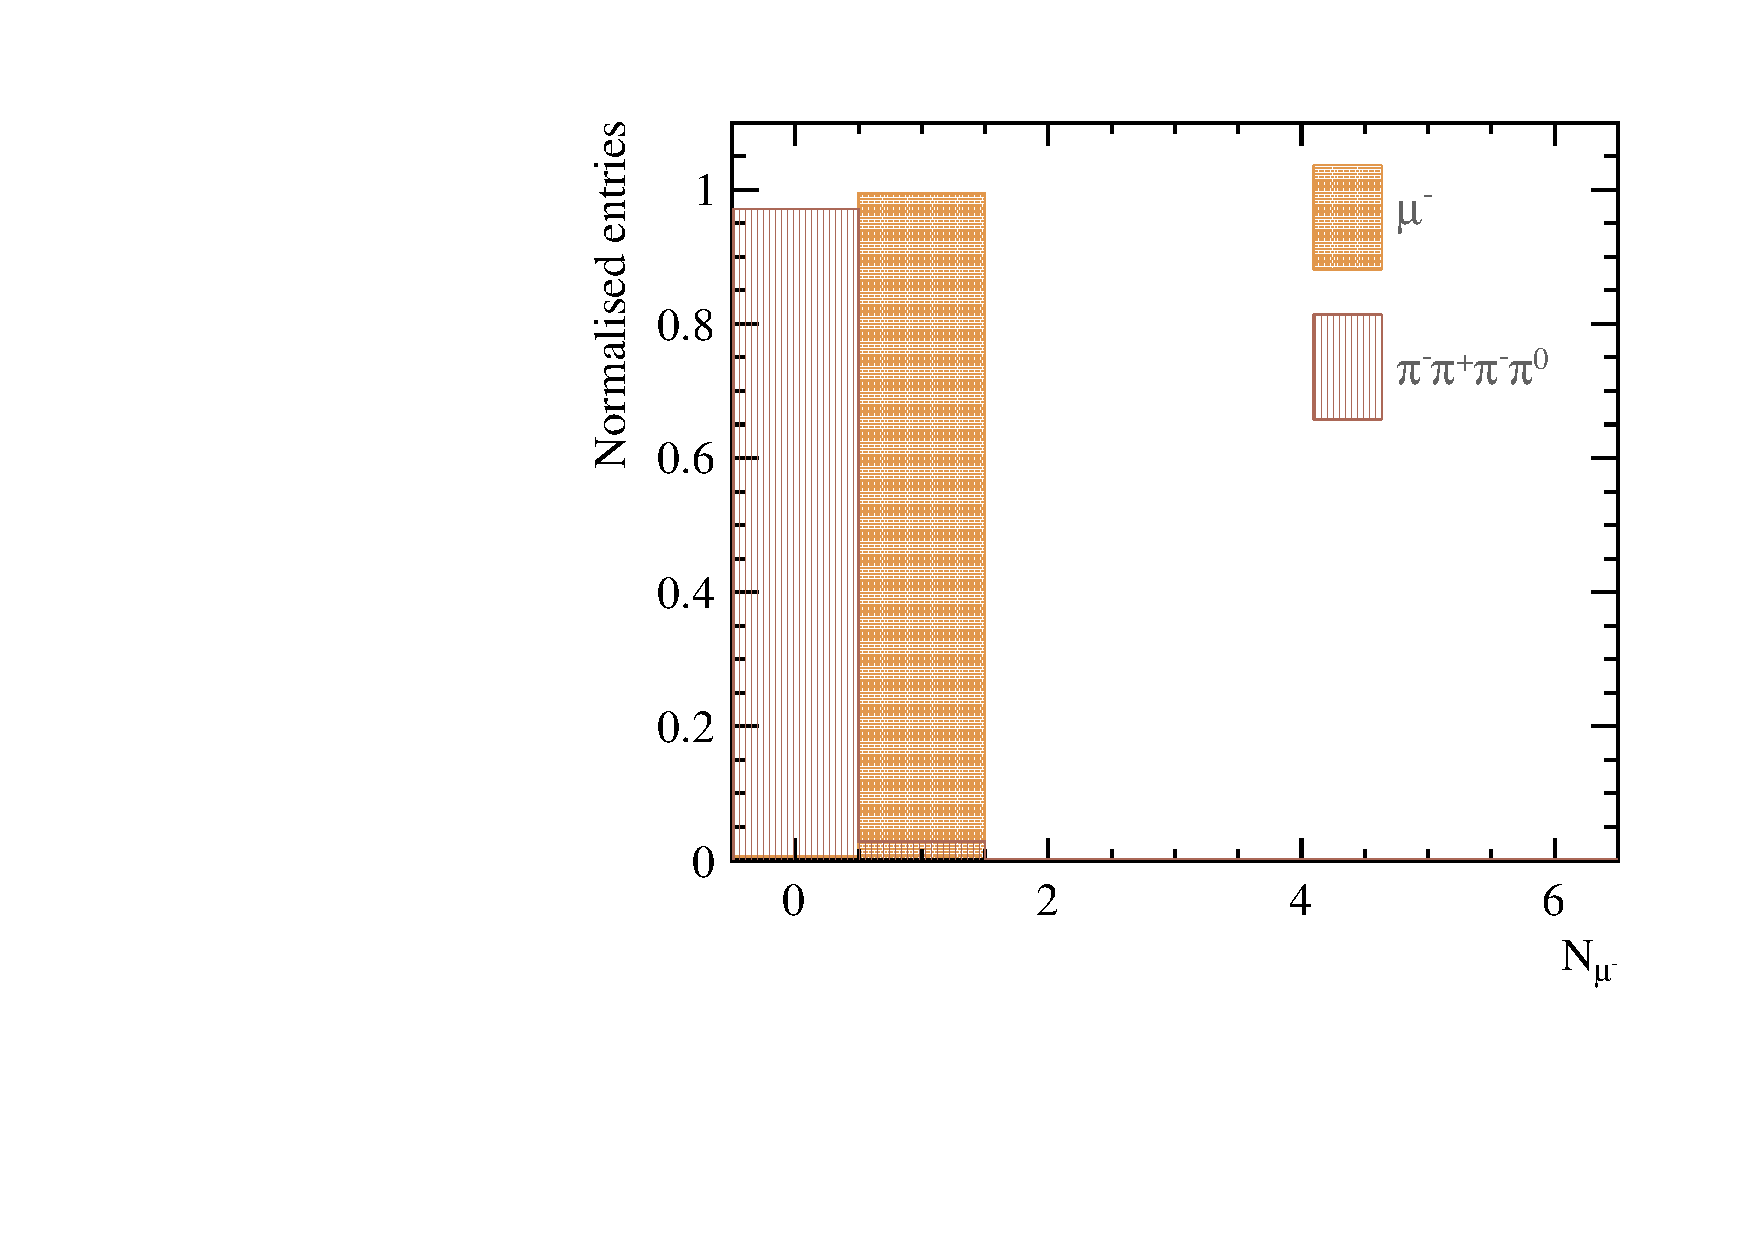
\includegraphics[width=\textwidth]{tau/var3/nMuon_100GeV_improved.pdf}
  \caption{}
  \label{fig:tauVarNMuon}
\end{subfigure}
\begin{subfigure}[b]{0.45\textwidth}
 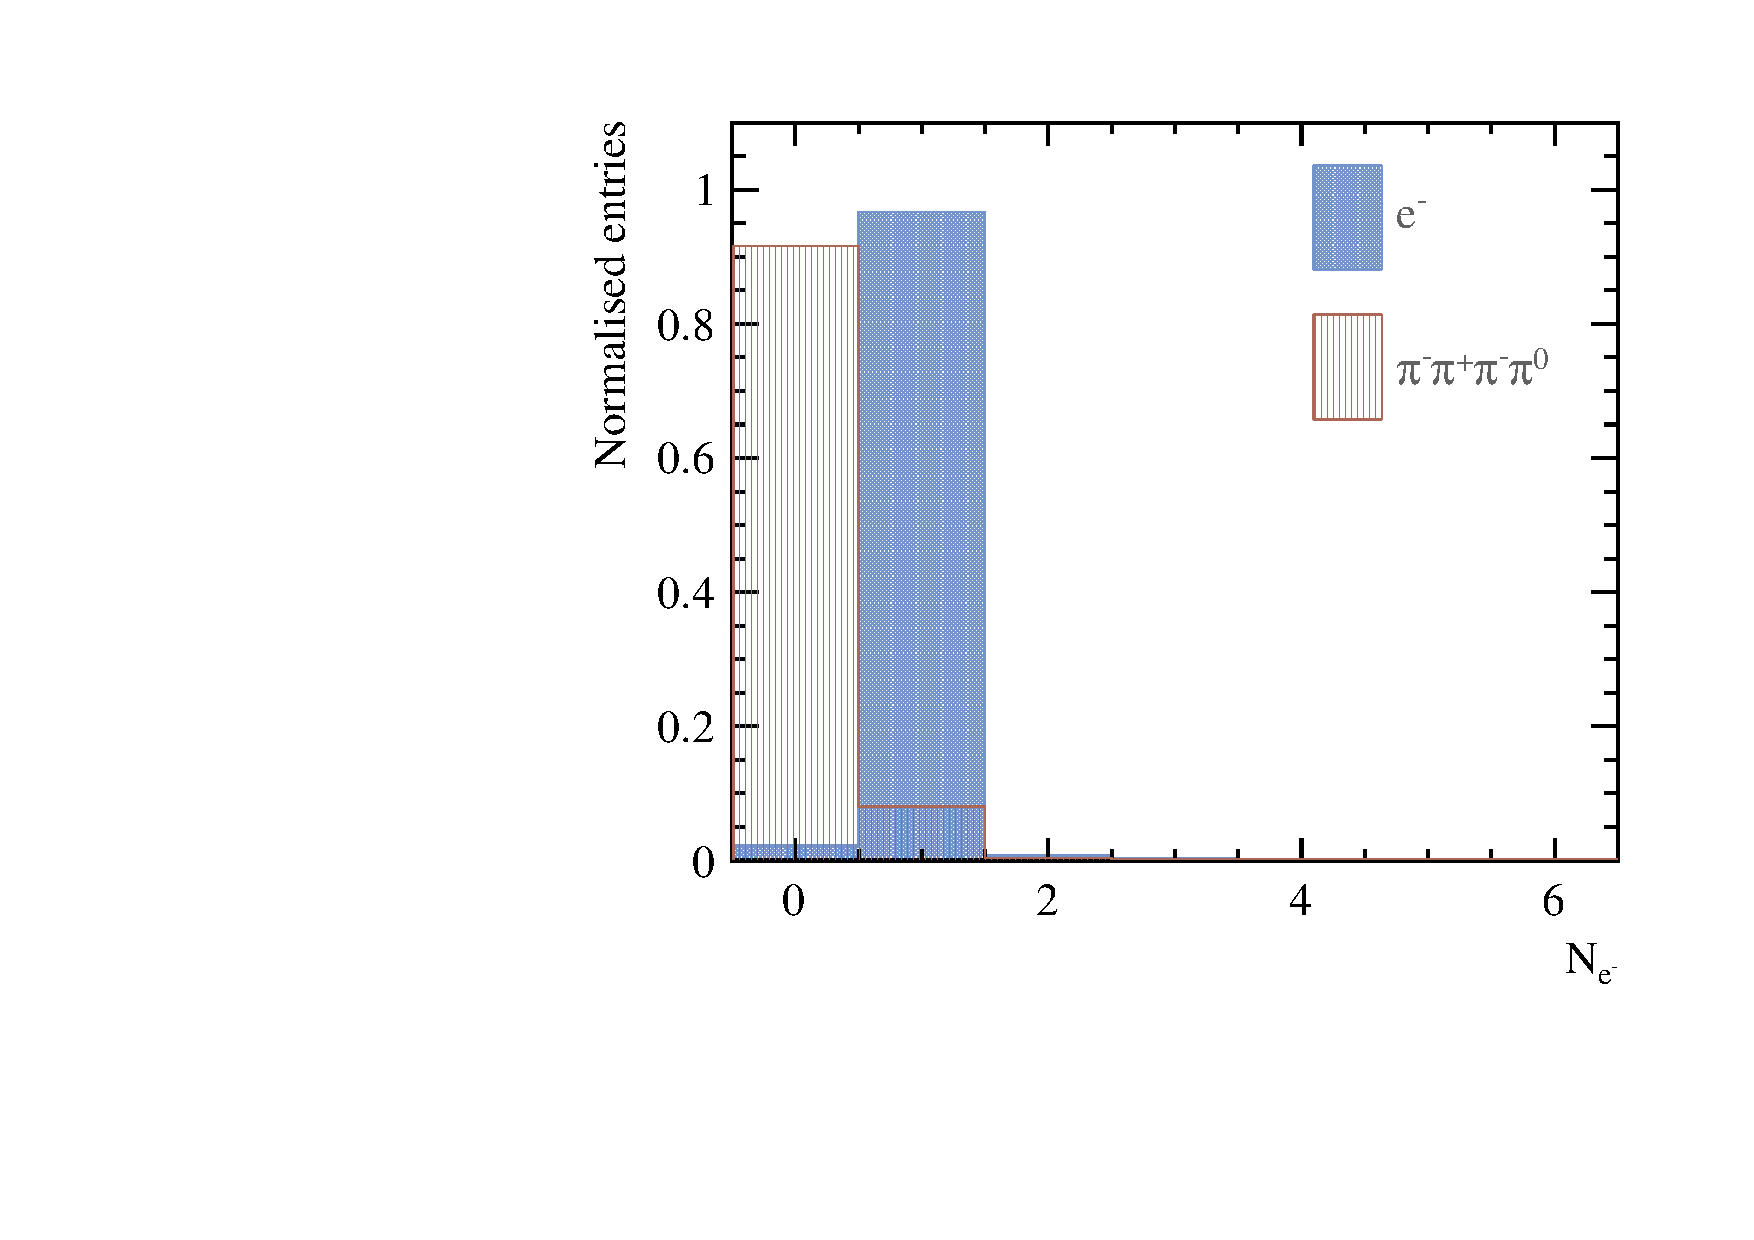
\includegraphics[width=\textwidth]{tau/var3/nElectron_100GeV_improved.pdf}
  \caption{}
  \label{fig:tauVarNElectron}
\end{subfigure}
\begin{subfigure}[b]{0.45\textwidth}
 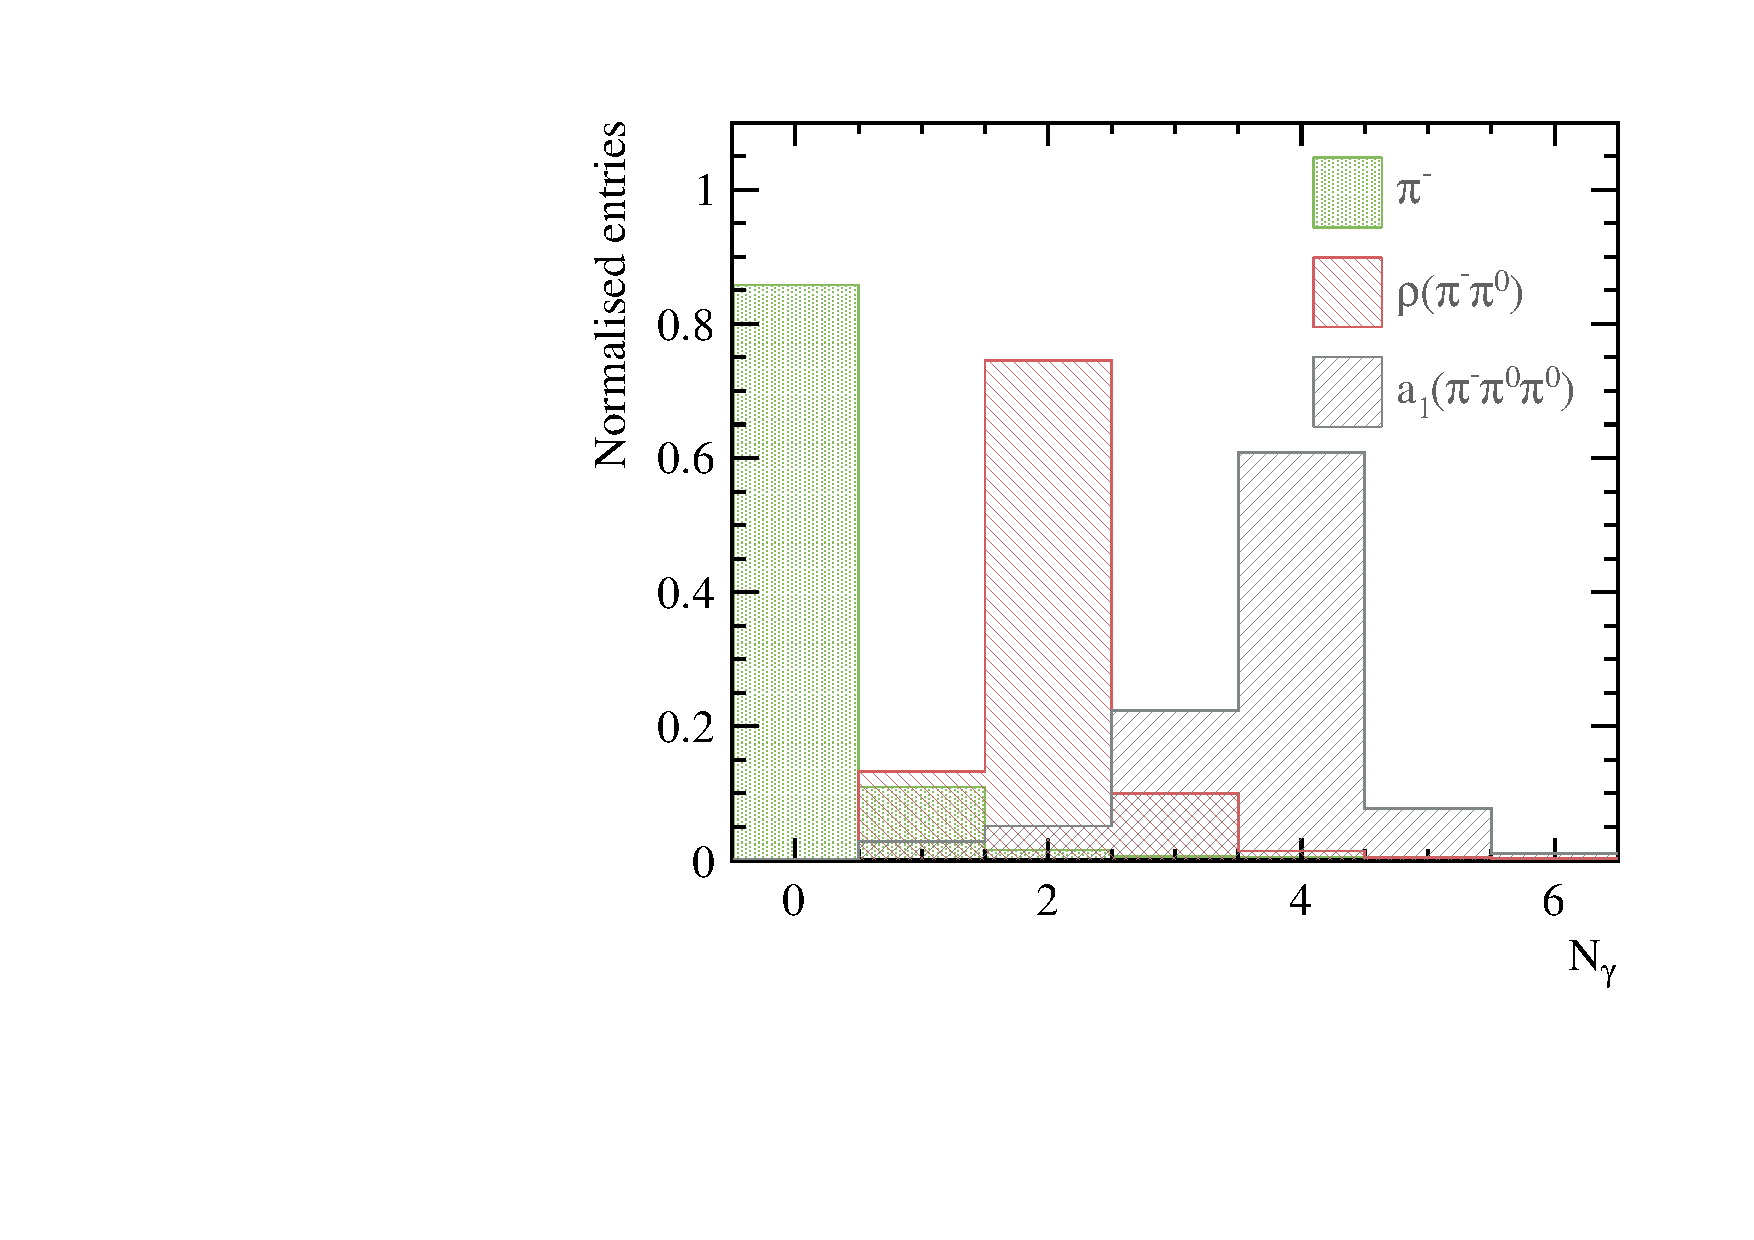
\includegraphics[width=\textwidth]{tau/var3/nPhoton_100GeV_improved.pdf}
  \caption{}
  \label{fig:tauVarNPhoton}
\end{subfigure}
\caption
{Distributions of  the number of reconstructed particles of different types: a)  charged particles (${N}_{\charge}$); b) muons (${N}_{\Pmu}$); c) electrons (${N}_{\Pe}$); and d)  photons (${N}_{\Pgg}$). The particle ID information comes from the output of the \pandora reconstruction. The area under the curve for each decay mode is normalised to unity.}
\label{fig:tauVar1}
\end{figure}

% and the overlap between \decayRhoShort and \decayAiPhotonShort is around 15\%. ${N}_{\Pgg}$ can also separate two 3-prong final states.
%${N}_{\Pmu}$, ${N}_{\Pe}$, ${N}_{\Pgpm}$ are useful to identify two leptonic final states, and further separate 3-prong final states from 1-prong final states.
%This is an excellent variable to separate 1-prong and 3-prong final states.  An orthogonal measurement is the number of reconstructed photons,  ${N}_{\Pgg}$, shown in \Figure{fig:tauVarNPhoton}.

\subsection{Invariant mass variables}

Five invariant mass variables are used in the MVA classification: the invariant mass of all reconstructed particles ($m_{vis}$); the invariant mass of all reconstructed charged particles ($m_{\charge}$); the invariant mass of all reconstructed neutral particles ($m_{\neutral}$); the invariant mass of all reconstructed photons ($m_{\Pgg}$); and the invariant mass of all reconstructed  charged pions ($m_{\Pgpm}$).

\FIGURE{fig:tauVarMVis} shows the distributions of the invariant masses of all reconstructed particles  for different tau decay modes. Peaks in the invariant mass distributions can be seen for the \Prho and \Pai decay modes. \FIGURE{fig:tauVarMNeutral} shows the distributions of the invariant masses of all reconstructed neutral particles  for different tau decay modes. Differences in the distributions for  the \Prho and \Pai decay modes can be seen.



%Invariant masses of different particles are good at characterising different final states. \FIGURE{fig:tauVarMVis} shows the invariant mass of the system. Clear reasonable peaks can be seen for \Prho and \Pai. The mass peak of  \decayAiPionFinalStateShort are much higher. $m_{\charge}$ and $m_{\neutral}$ are invariant masses of charged and neutral particles respectively. They separate final states with neutral particles from those without neutral particles. Similarly, $m_{\Pgg}$ and $m_{\Pgpm}$ identify final states with photons and with \Pgpm respectively.



\begin{figure}[htbp]
\centering
% \begin{center}/\end{center} takes some additional vertical space
\begin{subfigure}[b]{0.45\textwidth}
 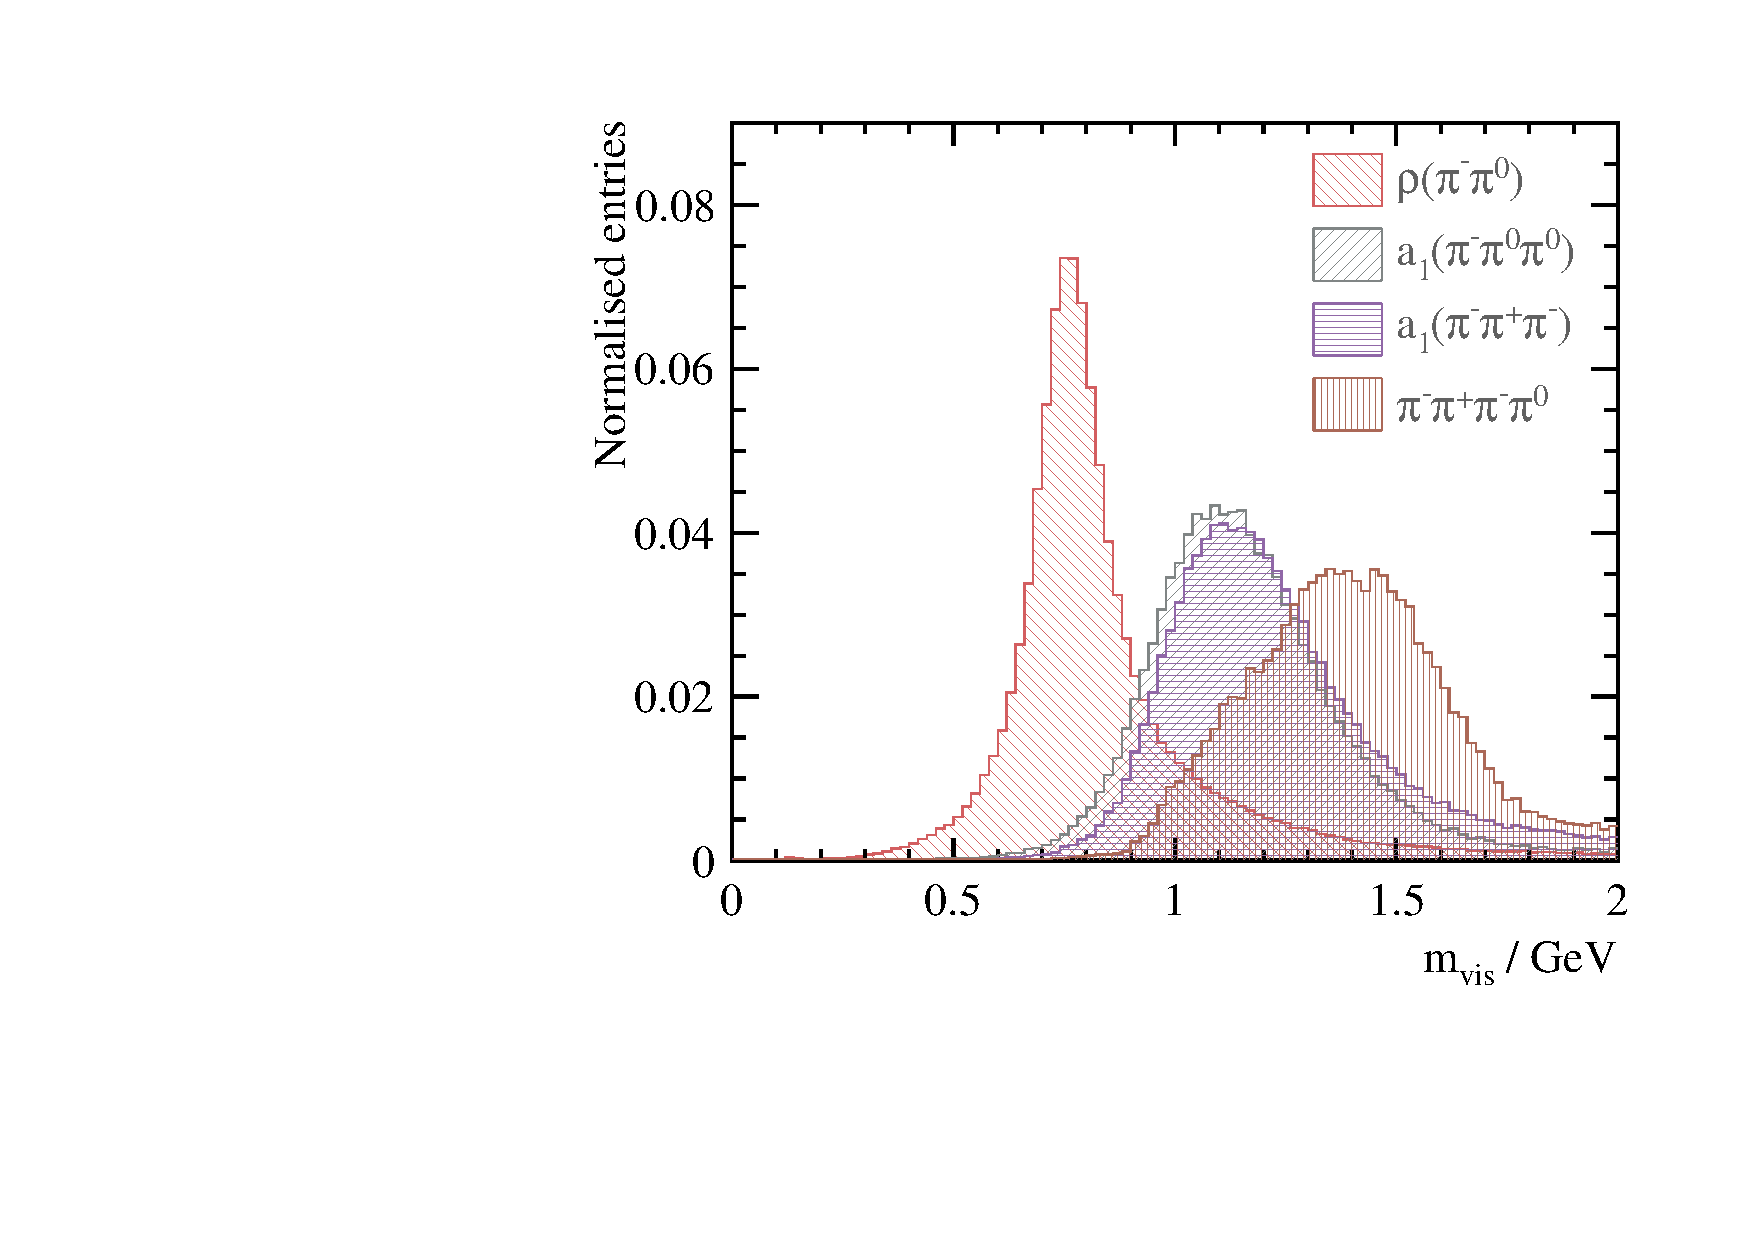
\includegraphics[width=\textwidth]{tau/var3/mVis_100GeV_improved_zoom.pdf}
  \caption{}
  \label{fig:tauVarMVis}
\end{subfigure}
\begin{subfigure}[b]{0.45\textwidth}
 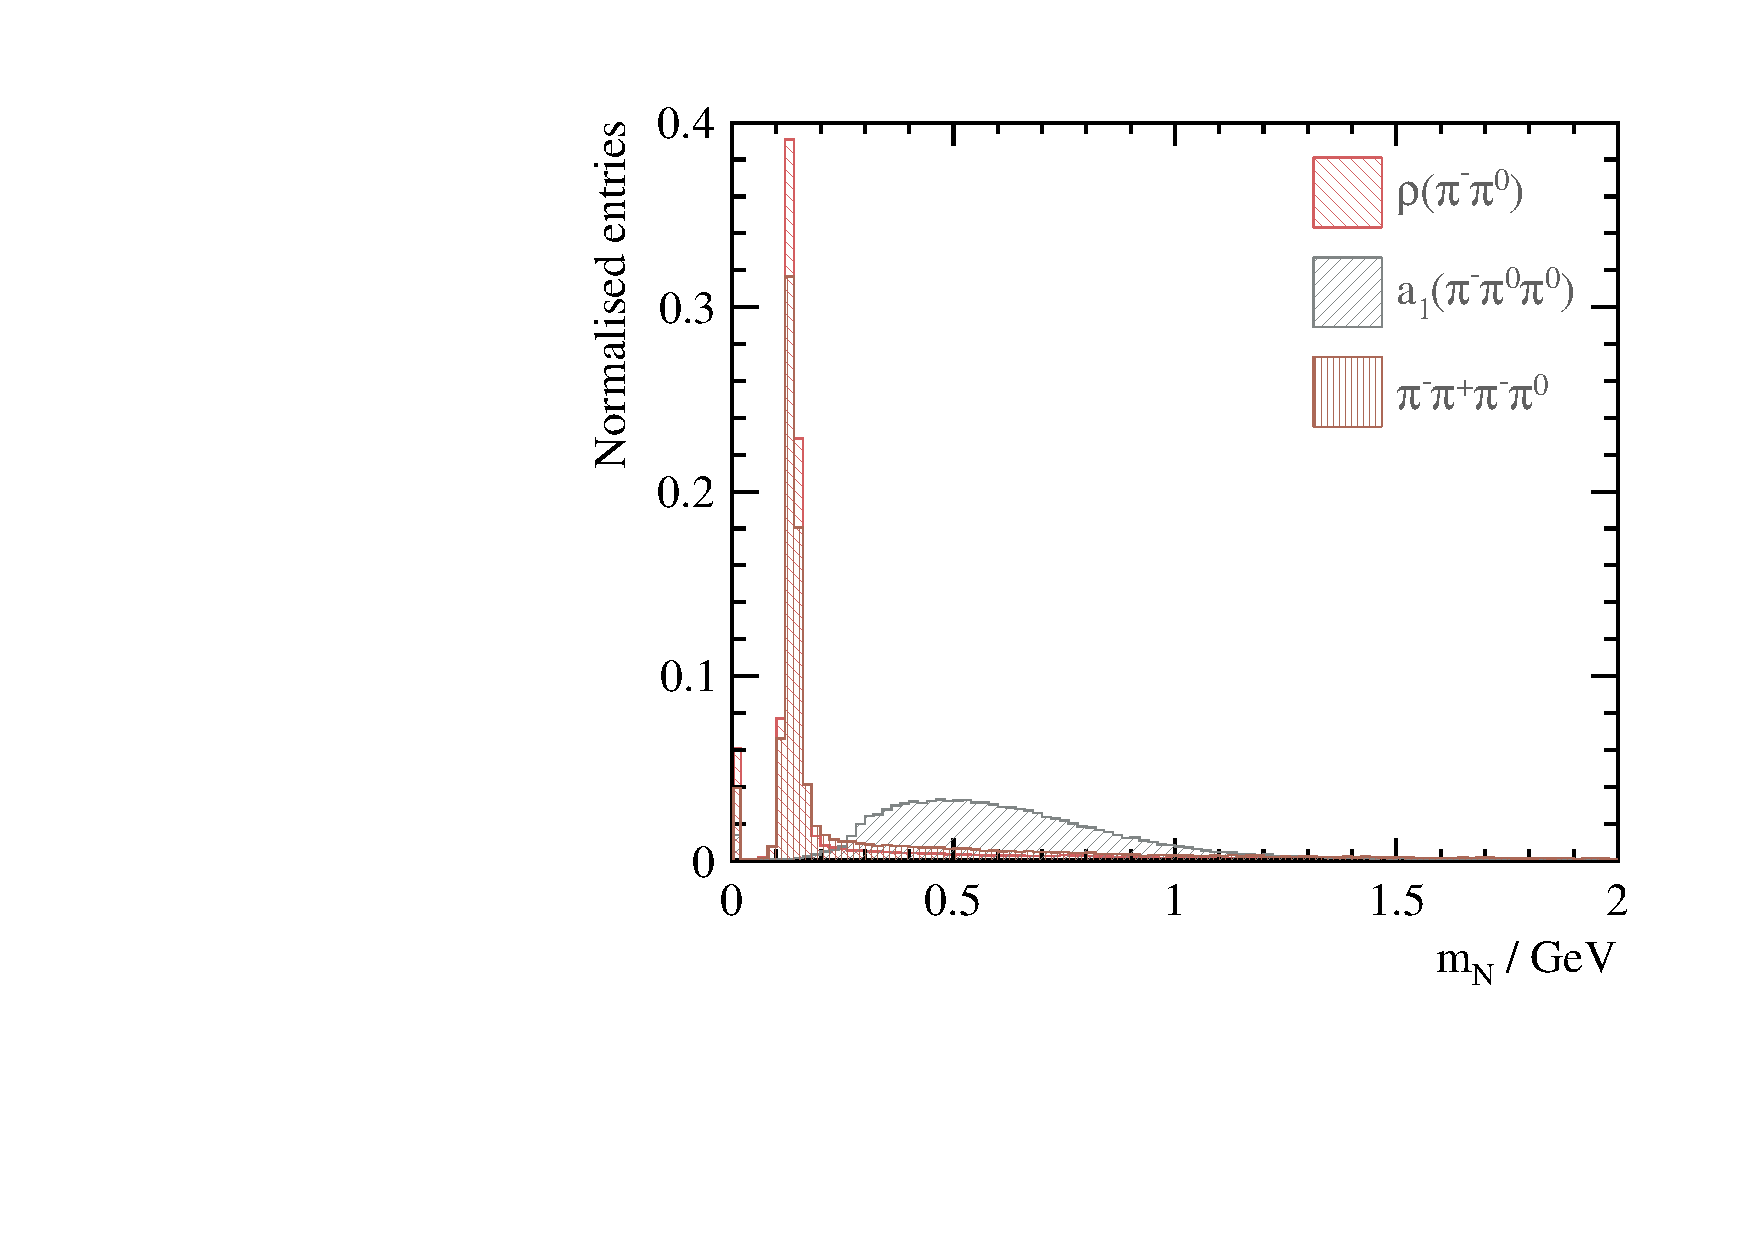
\includegraphics[width=\textwidth]{tau/var3/mNeutral_100GeV_improved_zoom.pdf}
  \caption{}
  \label{fig:tauVarMNeutral}
\end{subfigure}
\caption
{Distributions of  the invariant mass of  a) all particles (${m}_{vis}$); and b) all neutral particles (${m}_{\neutral}$). The particle ID information comes from the output of the \pandora reconstruction. The area under the curve for each decay mode is normalised to unity.}
\label{fig:tauVar2}
\end{figure}

\subsection{Energy variables}

Energy information helps to further separate different tau decay modes. Six energy variables are used in the MVA classification: the normalised total energy of all reconstructed particles ($\tilde{E}_{vis}$); the normalised total energy of charged particles ($\tilde{E}_{\charge}$); the normalised total energy of muons ($\tilde{E}_{\Pmu}$); the normalised total energy of electrons ($\tilde{E}_{\Pe}$); the normalised total energy of photons ($\tilde{E}_{\Pgg}$); and the normalised total energy of charged pions ($\tilde{E}_{\Pgpm}$). All variables are normalised relative to the energy of the associated tau lepton, i.e. $\tilde{E}_{vis} = E_{vis} / E_{\Ptau}$, where $E_{vis} $ is the total energy of all reconstructed particles and $E_{\Ptau}$ is the energy of the associated tau lepton.  $E_{\Ptau}$ is obtained from the generated value, i.e. 50\,GeV.


\FIGURE{fig:tauVarEVis} and \Figure{fig:tauVarEPhoton} show distributions of the normalised energies of all reconstructed particles and photons respectively for different tau decay modes. Differences in the distributions for  different tau decay modes can be seen. The cut-off at 0.1 for the $\tilde{E}_{vis}$ distribution is due to the pre-selection of  $E_{vis}^{MC}>5$\,GeV, which corresponds to  $\tilde{E}_{vis}>0.1$.



\begin{figure}[htbp]
\centering
% \begin{center}/\end{center} takes some additional vertical space
\begin{subfigure}[b]{0.45\textwidth}
 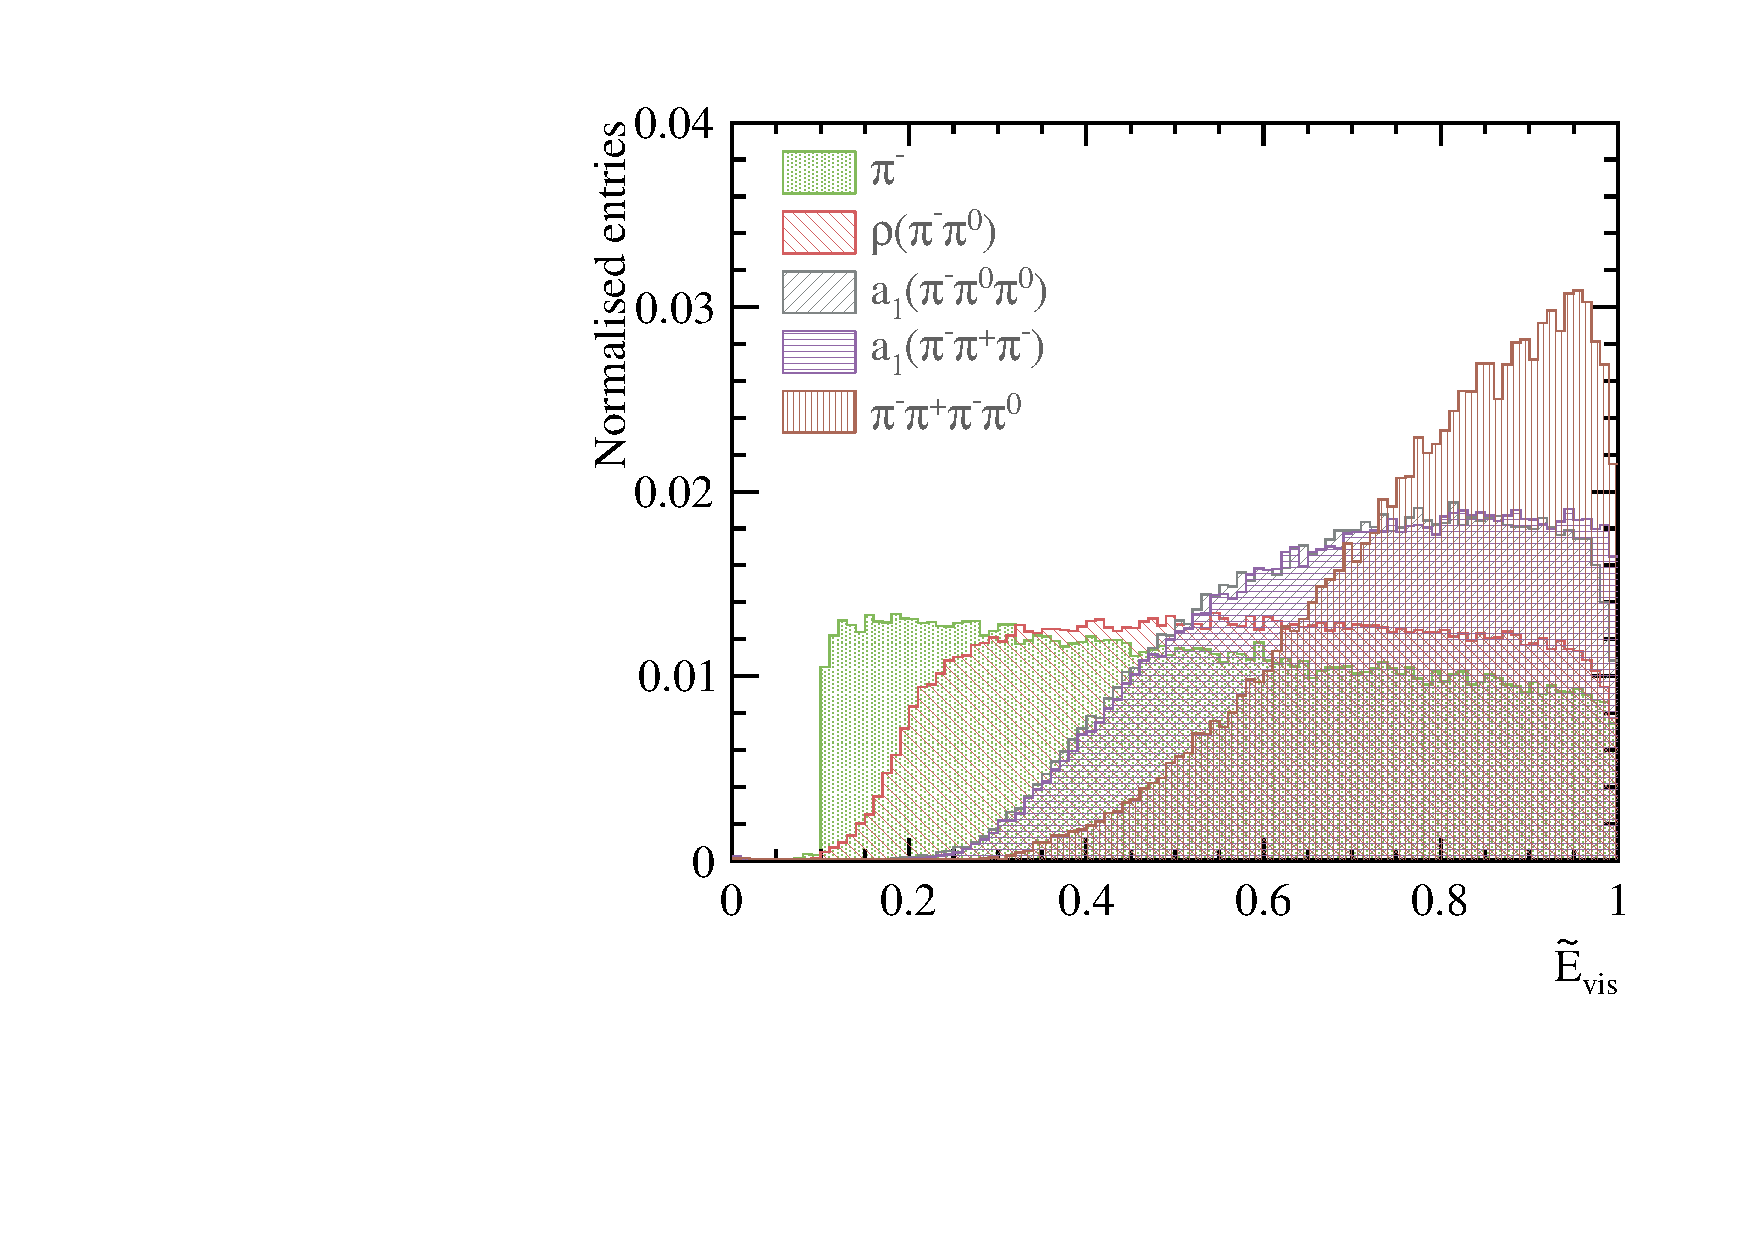
\includegraphics[width=\textwidth]{tau/var3/eVisRatio_100GeV_improved_zoom.pdf}
  \caption{}
  \label{fig:tauVarEVis}
\end{subfigure}
\begin{subfigure}[b]{0.45\textwidth}
 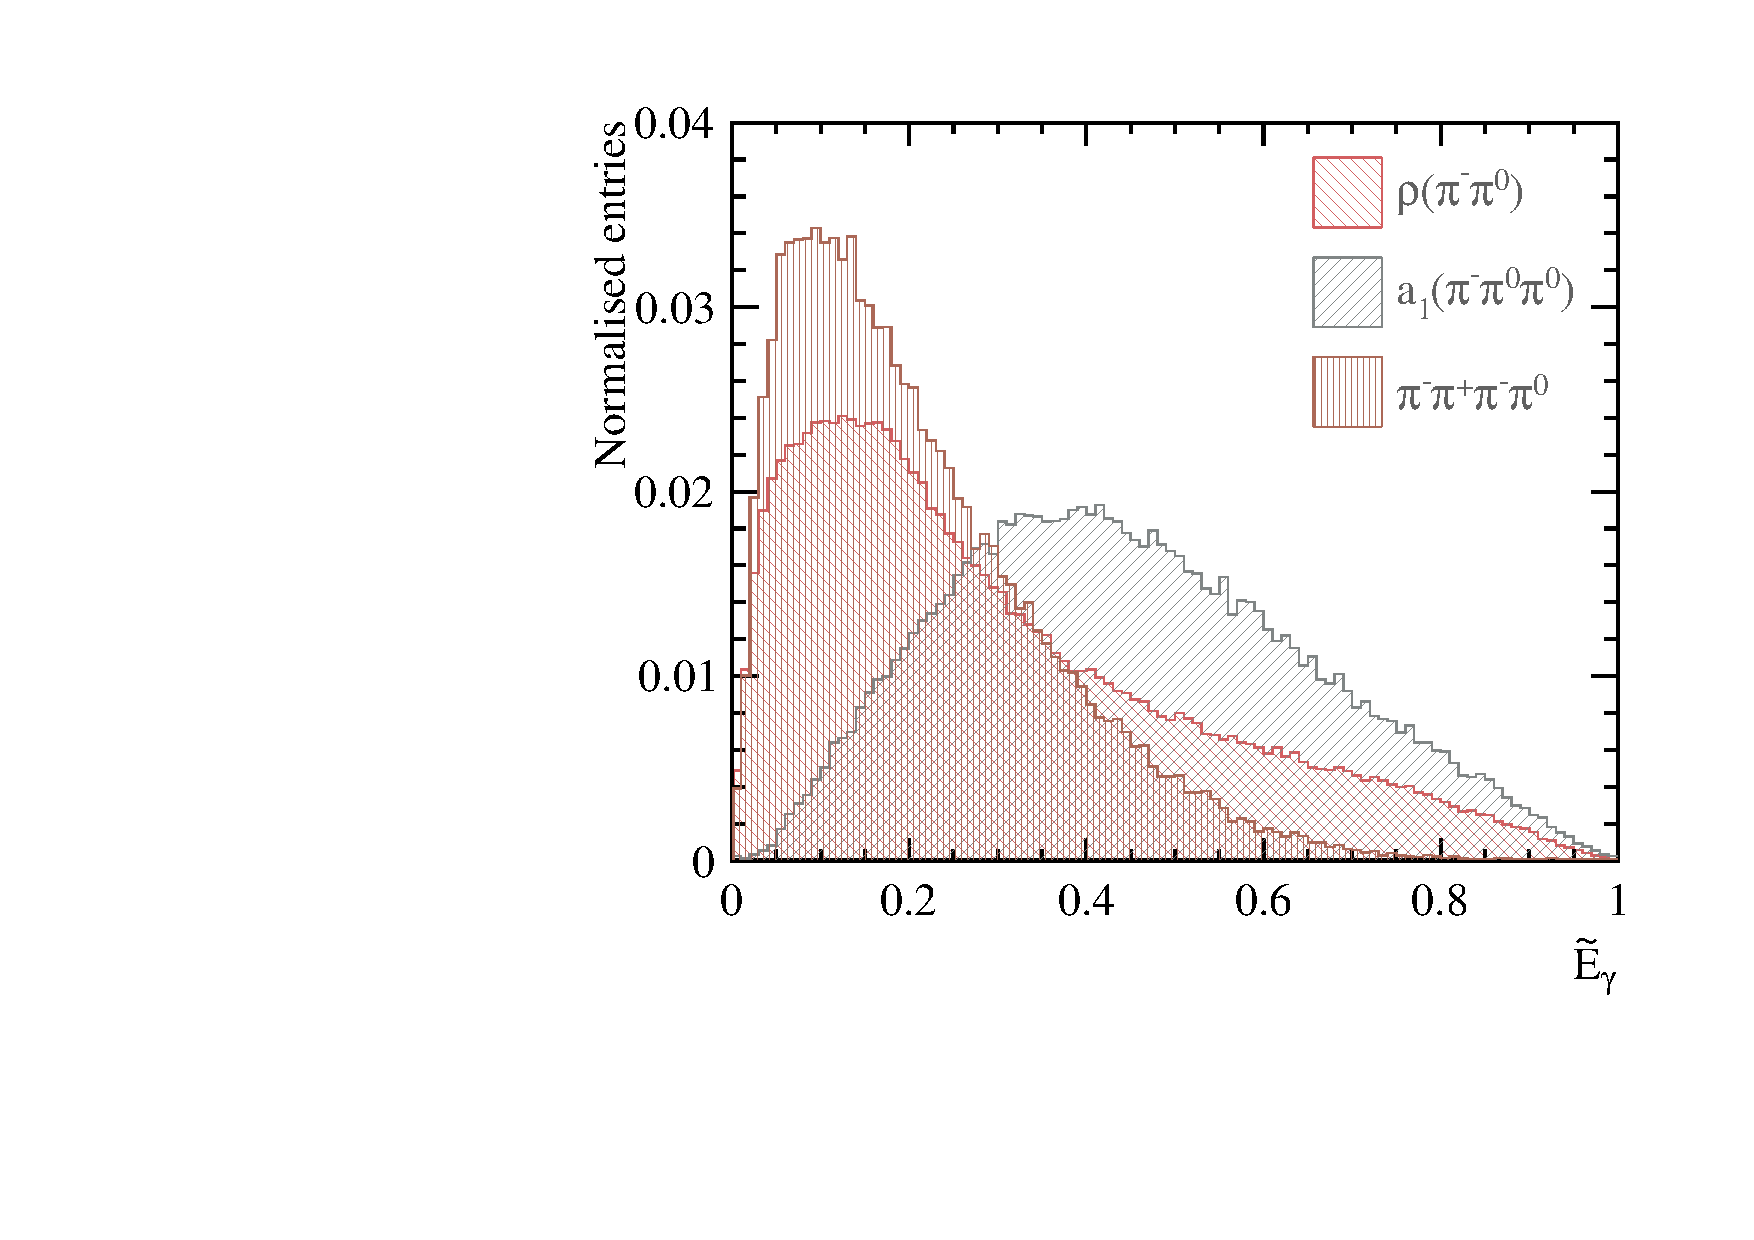
\includegraphics[width=\textwidth]{tau/var3/ePhotonRatio_100GeV_improved_zoom.pdf}
  \caption{}
  \label{fig:tauVarEPhoton}
\end{subfigure}
\caption
{Distributions of  the normalised energies of a) all reconstructed particles ($\tilde{E}_{vis}$); and b) all reconstructed  photons ($\tilde{E}_{\Pgg}$). The particle ID information comes from the output of the \pandora reconstruction. The area under the curve for each decay mode is normalised to unity.}
\label{fig:tauVar3}
\end{figure}

\subsection{Calorimetric energy variables}
% { $E^{\ECAL}_{\charge} / E_{\charge}$,  $ E^{\ECAL} / E$ } \\

Two calorimetric energy variables are used in the MVA classification: the fraction of the energy  deposited in the \ECAL divided by the  energy deposited in the \ECAL and \HCAL, where only calorimetric deposits associated with charged particles are considered ($E^{\ECAL}_{\charge} / E_{\charge}$); and the fraction of the energy  deposited in the \ECAL divided by the  energy deposited in the \ECAL and \HCAL for all particles ($E^{\ECAL} / E$). These  two variables help to improve the identification of electron and muon decay modes. \FIGURE{fig:tauVar4} show distributions of  $E^{\ECAL}_{\charge} / E_{\charge}$ and $E^{\ECAL} / E$ for different decay modes. An electron typically deposits over 95\% of its energy in the \ECAL, and a muon typically deposits 5\% to 20\% of its energy in the \ECAL. The difference between $E^{\ECAL}_{\charge} / E_{\charge}$ and  $E^{\ECAL} / E$ is that photons and neutral hadrons, which deposit most of their energies in the \ECAL and in the \HCAL respectively, are not included in the calculation of $E^{\ECAL}_{\charge} / E_{\charge}$.



\begin{figure}[htbp]
\centering
% \begin{center}/\end{center} takes some additional vertical space
\begin{subfigure}[b]{0.45\textwidth}
 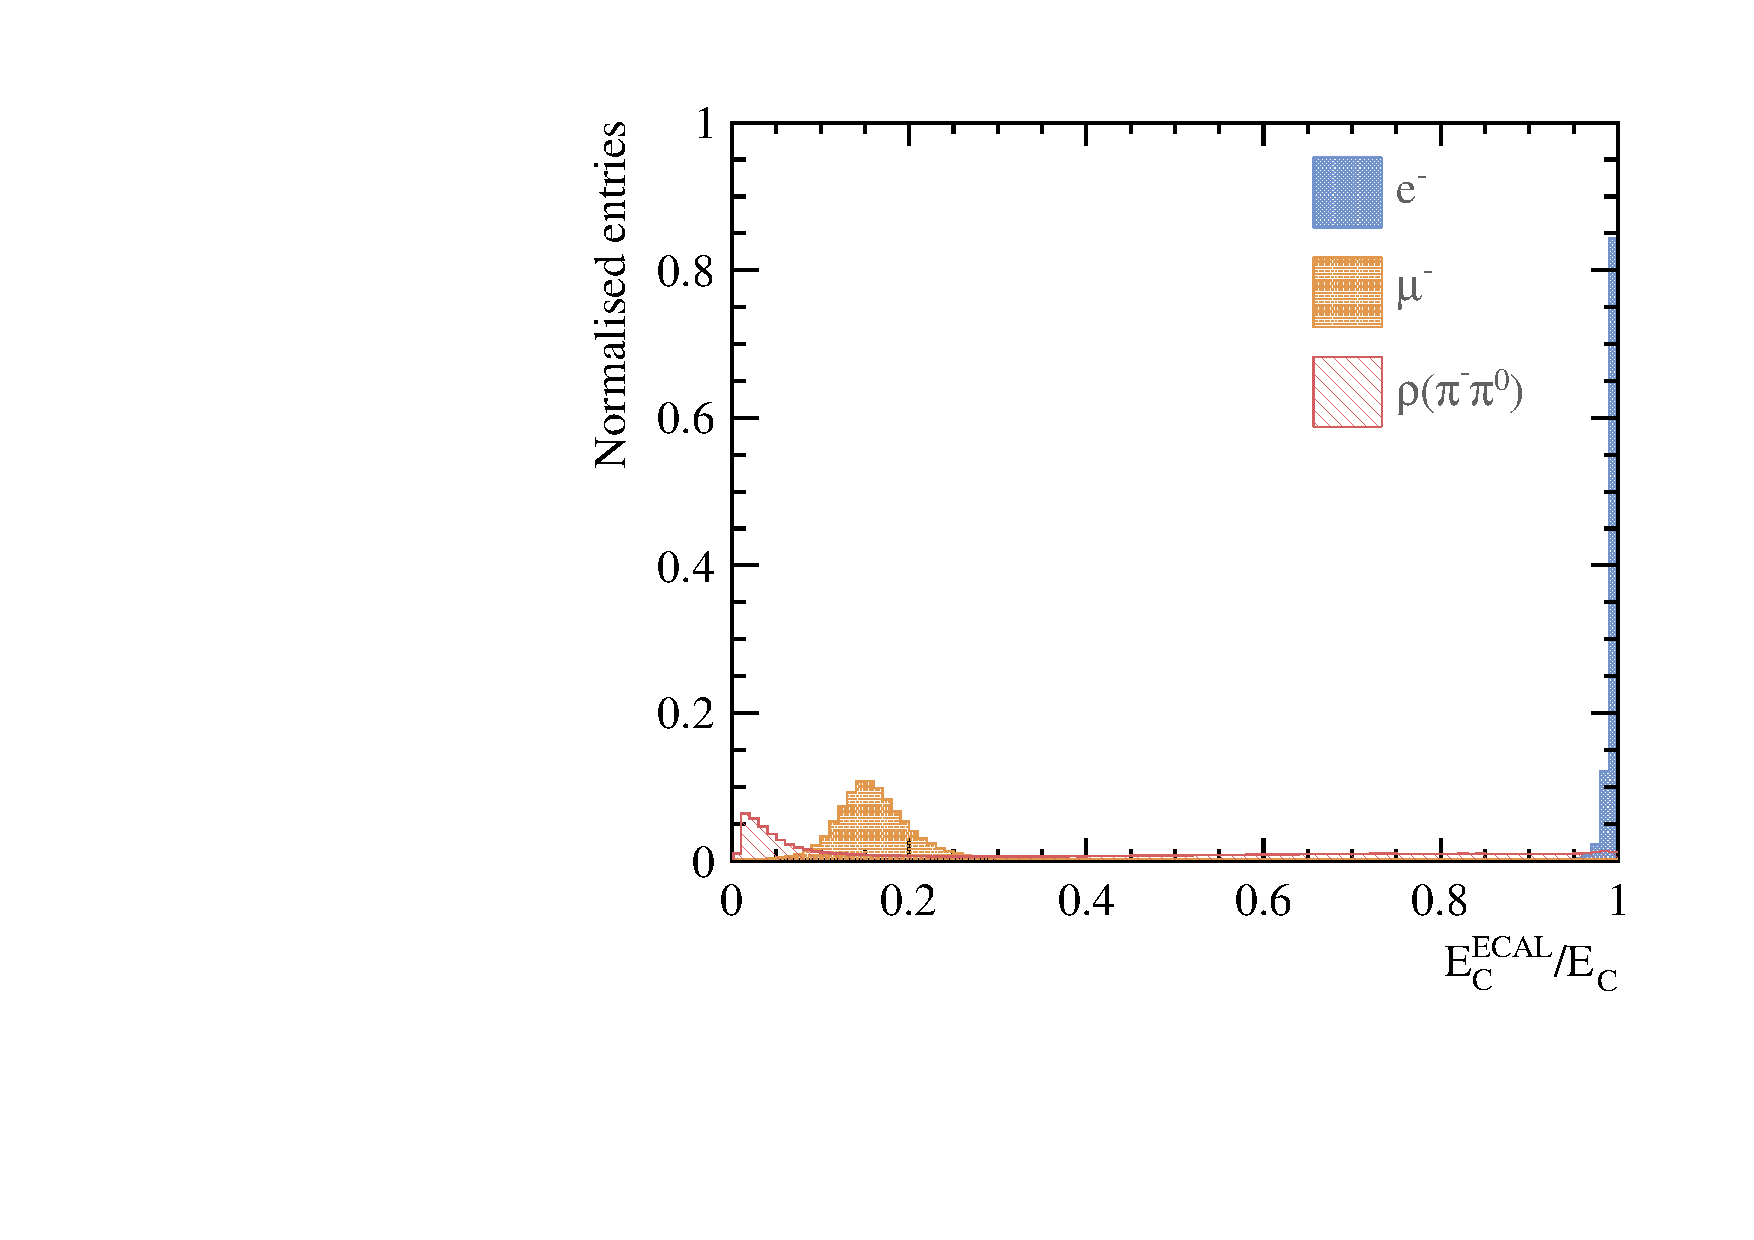
\includegraphics[width=\textwidth]{tau/var3/EEHCalRatio_100GeV_improved}
  \caption{}
  \label{fig:tauVarEEcalRatio}
\end{subfigure}
\begin{subfigure}[b]{0.45\textwidth}
 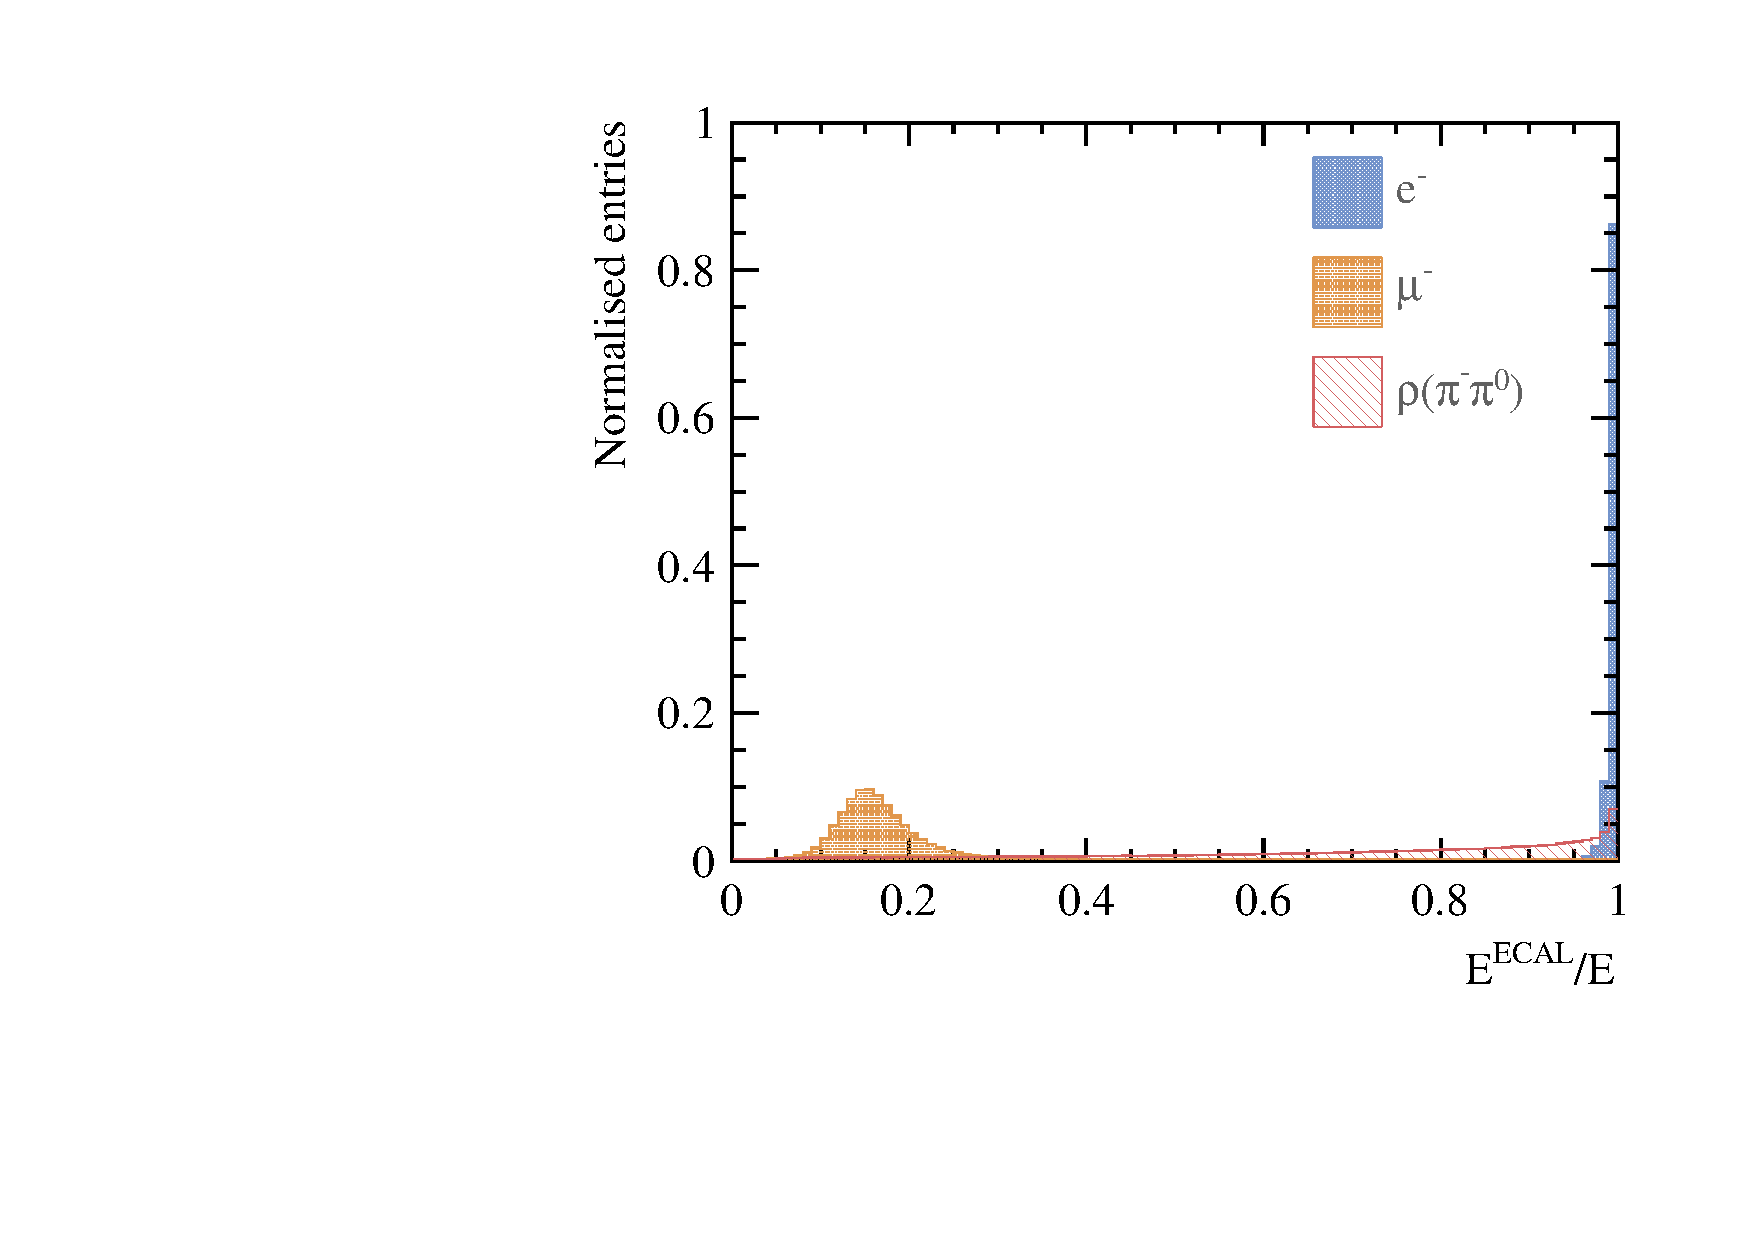
\includegraphics[width=\textwidth]{tau/var3/EEHCalAllRatio_100GeV_improved}
  \caption{}
  \label{fig:tauVarEEcalRatioAll}
\end{subfigure}
\caption
{Distributions of  the fraction of the energy  deposited in the \ECAL divided by the  energy deposited in the \ECAL and \HCAL, a) where only calorimetric deposits associated with charged particles are considered ($E^{\ECAL}_{\charge} / E_{\charge}$); and b) for all reconstructed particles ($ E^{\ECAL} / E$). The particle ID information comes from the output of the \pandora reconstruction. The area under the curve for each decay mode is normalised to unity.}
\label{fig:tauVar4}
\end{figure}

\subsection{\texorpdfstring{\decayRhoShort and \decayAiPhotonShort} \, resonances variables}


%\section{\texorpdfstring{\decayRhoShort and \decayAiPhotonShort} \, resonances reconstruction}
%\label{sec:tauResonance}

By utilising the photon identification potential of the highly granular \ECAL, the identification of the \decayRhoShort and \decayAiPhotonShort decay modes is enhanced  by reconstructing the \Prho and \Pai invariant masses. For decays with at least one charged pion and one photon, the reconstruction selects the combination of charged pions and photons that have a invariant mas mosts consistent with the \Prho or \Pai mass.



%The identification of the \decayRhoShort and \decayAiPhotonShort decay modes is enhanced  by reconstructing the \Prho and \Pai invariant mass. The


%The \decayRhoShort and \decayAiPhotonShort decay modes identification is enhanced  by reconstructing the \Prho and \Pai invariant mass resonances.
% By selecting \Pgpm and photons consistent with \Prho mass, \decayRhoShort decay mode reconstruction is improved.
For example, the final state of the \decayRhoShort decay mode contains a \Pgpm and a \Ppizero, where  \pionToPhoton. The  \decayRhoShort decay mode hypothesis test is performed by selecting the combination of the charged pion and photons that gives the smallest value of a $\chi^{2}$ function:
\begin{equation}
\chi^{2} = {\left(\frac{m_{tot} -  m_{\Prho}}{\sigma_{\Prho}}\right)}^{2} + {\left(\frac{m_{\Pphoton_1\Pphoton_2} -  m_{\Ppizero}}{\sigma_{\Ppizero}}\right)}^{2} \,,
\label{eqn:tauRho}
\end{equation}
where $m_{\Pphoton_1\Pphoton_2}$ is the invariant mass of two photons; the variable $m_{tot}$ is the total invariant mass of the  two photons and one \Pgpm; $m_{\Prho}$ and $m_{\Ppizero}$ are the respective true masses of \Prho and \Ppizero; and $\sigma_{\Prho}$ and $\sigma_{\Ppizero}$ are the assumed mass resolutions. \FIGURE{fig:tauRho} shows the reconstructed invariant mass distributions for \Ppizero and \Prho in the \decayRhoShort decay mode, obtained by selecting reconstructed particles using the MC truth information.  A mass resolution of 20\% is an good approximation for the invariant masses of \Ppizero and \Prho, and this is used for $\sigma_{\Prho}$ and $\sigma_{\Ppizero}$.

%the mass resolution is assumed to be 20\%, i.e. $\sigma_{\Prho}/m_{\Prho}$ = $\sigma_{\Ppizero}/m_{\Ppizero}$ = 20\%. The decay mode is selected using the MC truth information.
% to find the corresponding reconstructed particles

The particle ID of charged pions and photons comes from the output of the \pandora reconstruction. The $\chi^{2}$ function works naturally if there are two reconstructed photons in a decay. If there are more than two photons in a decay, all combinations of two photons are considered and the combination with the smallest value of $\chi^2$ is chosen. If there is only one photon in a decay, the second term in the \Equation{eqn:tauRho} is dropped and $m_{tot}$ is the total invariant mass of one photon and one \Pgpm.

\begin{comment}
the $\chi^{2}$ function becomes:
\begin{equation}
\chi^{2} = {\left(\frac{m_{tot} -  m_{\Prho}}{\sigma_{\Prho}}\right)}^{2} \,,
\end{equation}
where $m_{tot}$ is the total invariant mass of one photon and one \Pgpm.
\end{comment}


\begin{figure}[htbp]
\centering
% \begin{center}/\end{center} takes some additional vertical space
\begin{subfigure}[b]{0.45\textwidth}
 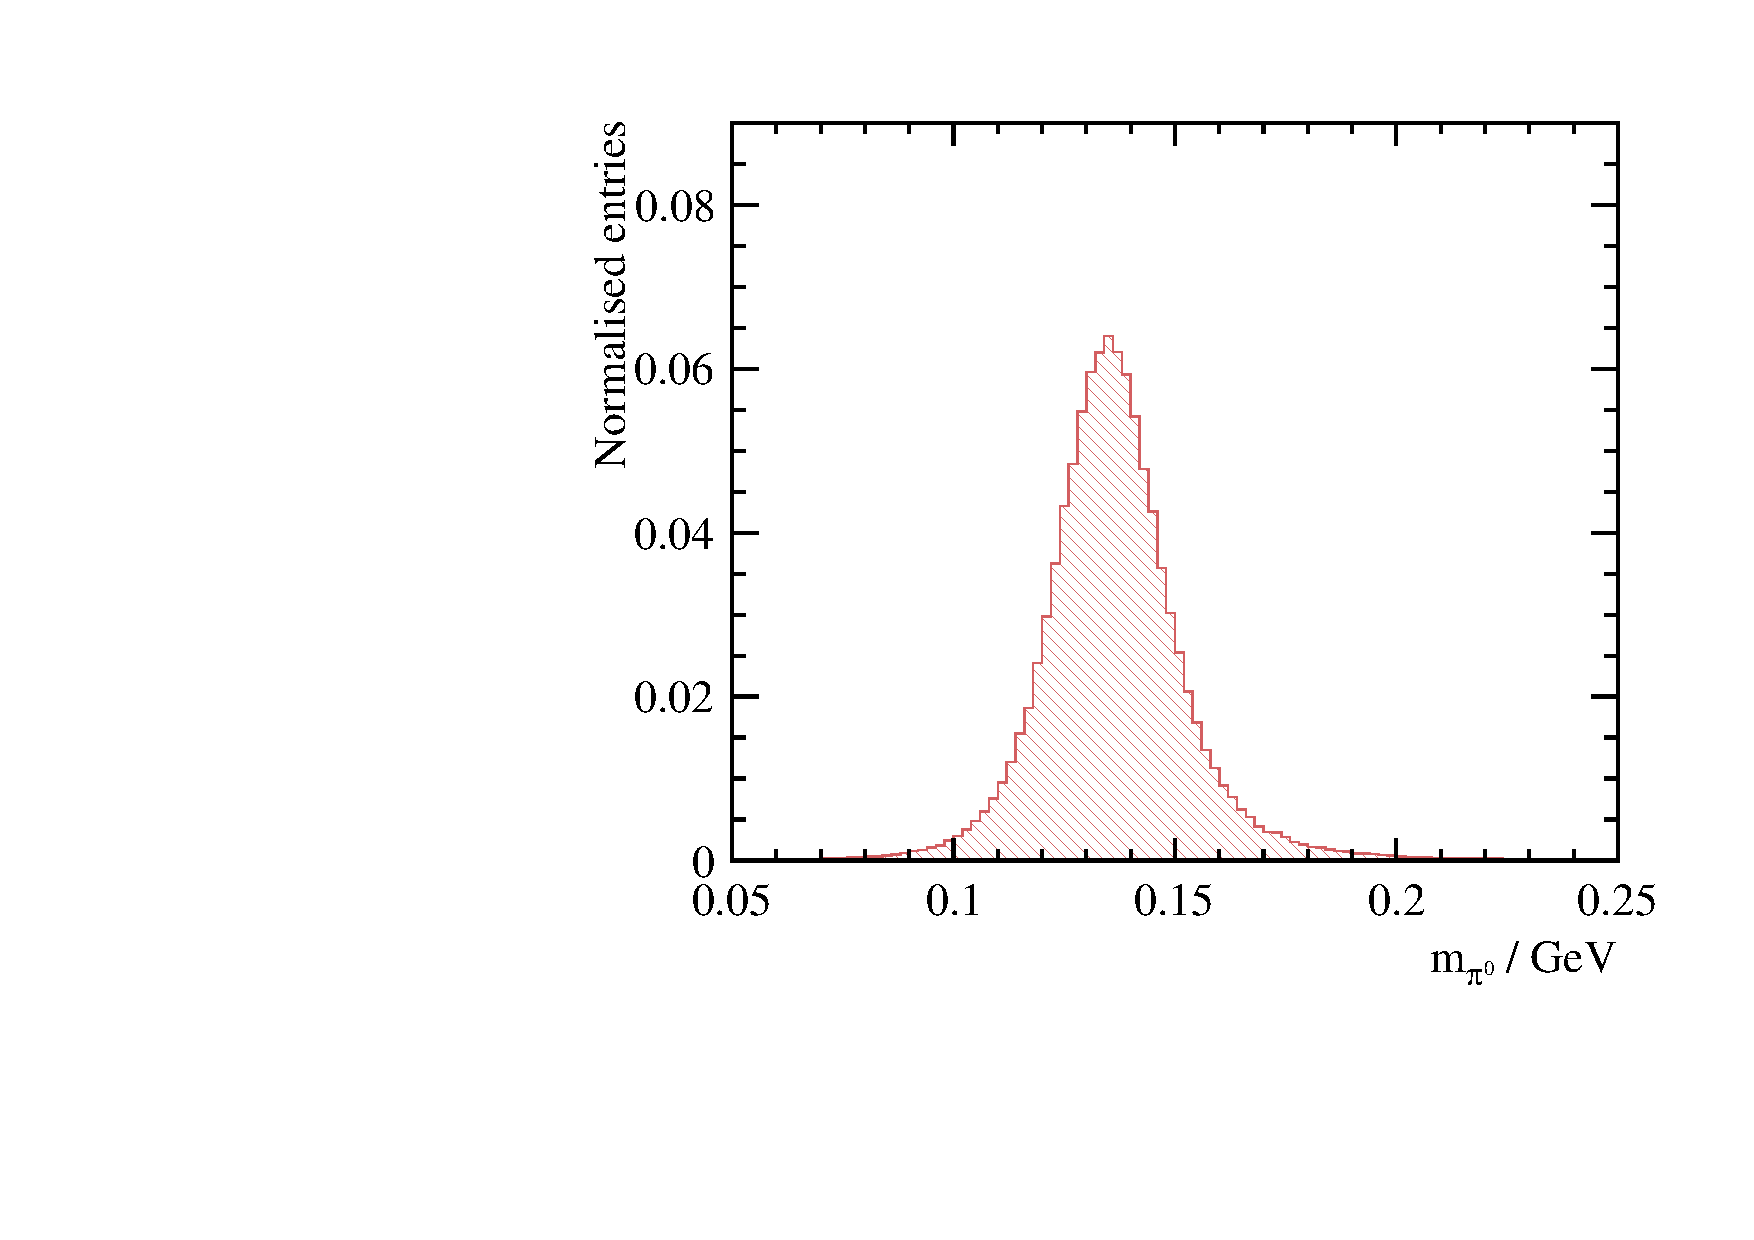
\includegraphics[width=\textwidth]{tau/var3/mPionRhoFit_100GeV_improved_zoom.pdf}
  \caption{}
  \label{fig:tauPionFromRho}
\end{subfigure}
\begin{subfigure}[b]{0.45\textwidth}
 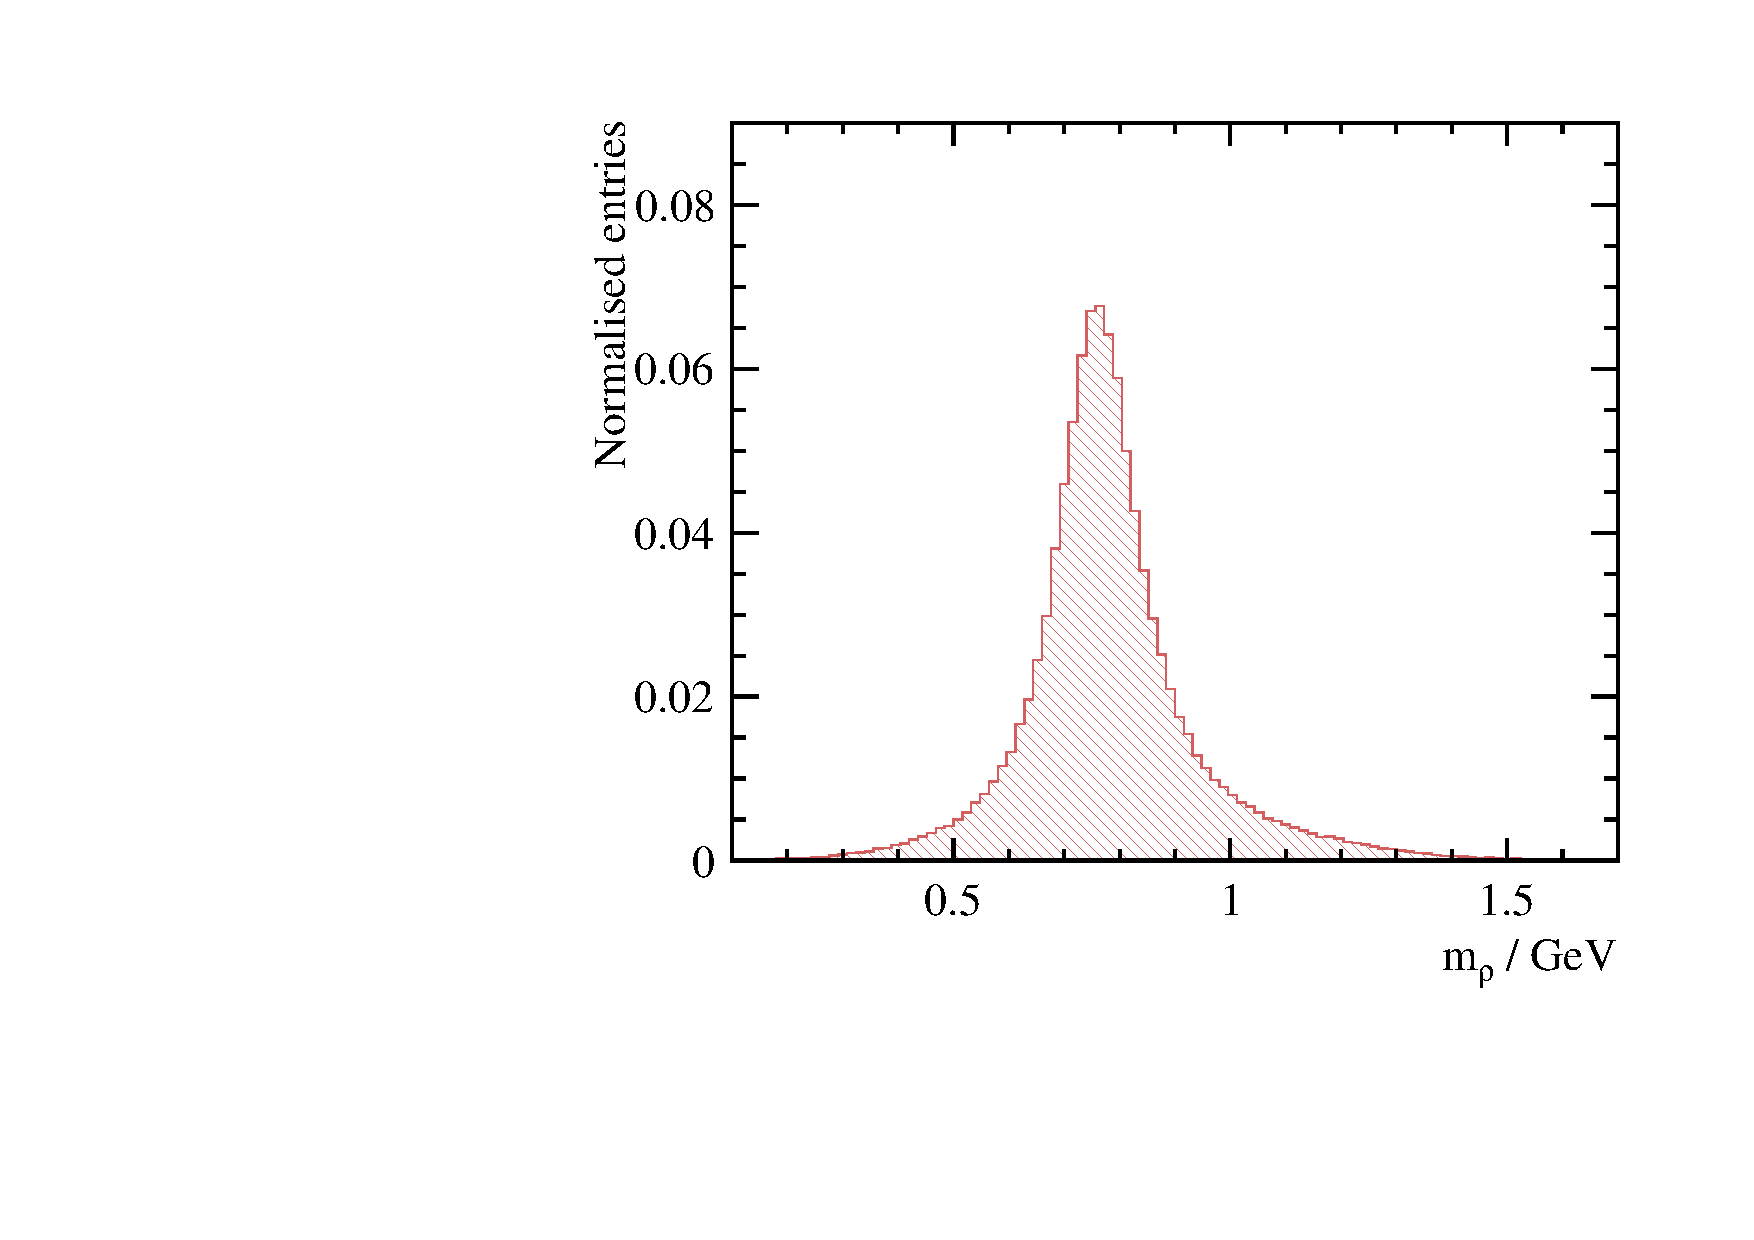
\includegraphics[width=\textwidth]{tau/var3/mRhoRhoFit_100GeV_improved_zoom.pdf}
  \caption{}
  \label{fig:tauRhoFromRho}
\end{subfigure}
\caption
{Reconstructed invariant mass distributions for the \Ppizero and \Prho in the \decayRhoShort decay mode. The reconstructed masses are obtained using the MC truth information to find the corresponding reconstructed particles. The area under the curve is normalised to unity.}
\label{fig:tauRho}
\end{figure}



% and $\sigma_{\Ppizero}$ are assumed

%the respective half widths of the invariant mass distributions of reconstructed \Prho and \Ppizero.



%The minimisation function is iterated over all combinations of photons and \Pgpm.




%By choosing the combination of photons and \Pgpm which minimises the  $\chi^{2}$ function, the fitted \Prho mass, $m_{tot}$, and the fitted \Ppizero mass, $m_{\Pphoton_1\Pphoton_2}$, are obtained.

The $\chi^2$ function of \Equation{eqn:tauRho} is modified for the \decayAiPhotonShort decay mode hypothesis test:
%The \decayAiPhotonShort decay mode identification can be enhanced using an similar minimisation function, $\chi^2$:
\begin{equation}
\chi^{2} = {\left(\frac{m_{tot} -  m_{\Pai}}{\sigma_{\Pai}}\right)}^{2} + {\left(\frac{m_{\Pphoton_1 \Pphoton_2} -  m_{\Ppizero}}{\sigma_{\Ppizero}}\right)}^{2}  + {\left(\frac{m_{\Pphoton_3 \Pphoton_4} -  m_{\Ppizero}}{\sigma_{\Ppizero}}\right)}^{2} \,,
\label{eqn:tauA1}
\end{equation}
where the \Prho mass has been replaced by the \Pai mass and other variables are defined in the same way as  previously. Four photons and one \Pgpm are required for this  $\chi^2$ function. To resolve the degeneracy between two photon pairs,  the requirement of $\absOf{ m_{\Pphoton_1\Pphoton_2} - m_{\Ppizero}} < \absOf{ m_{\Pphoton_3\Pphoton_4} - m_{\Ppizero}}$ is imposed.

If there are at least four photons in a decay, all combinations of four photons are considered and the combination with the smallest value of $\chi^2$ is chosen. If there are three photons in a decay, the last term in the \Equation{eqn:tauA1}  is dropped and the $\chi^{2}$ function becomes:
\begin{equation}
\chi^{2} = {\left(\frac{m_{tot} -  m_{\Pai}}{\sigma_{\Pai}}\right)}^{2} + {\left(\frac{m_{\Pphoton_1 \Pphoton_2} -  m_{\Ppizero}}{\sigma_{\Ppizero}}\right)}^{2}  \,,
\end{equation}
where $m_{tot}$ is the invariant mass of the charged pion and three photons and $m_{\Pphoton_1 \Pphoton_2}$ is the invariant mass of two photons. The combinations of photons are iterated.


If there are only two photons in a decay, either the reconstruction faied to reconstruct one photon pair or the reconstruction fails to reconstruct both photon pair. Hence two $\chi^2$ functions are used and the one with the smallest value is chosen. The first function is
\begin{equation}
\chi^{2} =\frac{1}{2} {\left(\frac{m_{tot} -  m_{\Pai}}{\sigma_{\Pai}}\right)}^{2} + \frac{1}{2} {\left(\frac{m_{\Pphoton_1 \Pphoton_2} -  m_{\Ppizero}}{\sigma_{\Ppizero}}\right)}^{2}  \,,
\label{eqn:tauA1TwoPhoton1}
\end{equation}
where $m_{tot}$ is the invariant mass of the charged pion and two photons and $m_{\Pphoton_1 \Pphoton_2}$ is the invariant mass of two photons. The second function is
\begin{equation}
\chi^{2} = {\left(\frac{m_{tot} -  m_{\Pai}}{\sigma_{\Pai}}\right)}^{2} \,,
\label{eqn:tauA1TwoPhoton2}
\end{equation}
where $m_{tot}$ is the invariant mass of the charged pion and two photons.


If there is only one photon in a decay,  $m_{tot}$ is the invariant mass of the charged pion and the photon.

\begin{comment}
the $\chi^{2}$ function becomes:
\begin{equation}
\chi^{2} = {\left(\frac{m_{tot} -  m_{\Pai}}{\sigma_{\Pai}}\right)}^{2} \,,
\end{equation}
where $m_{tot}$ is the invariant mass of the charged pion and the photon.
\end{comment}
% If there is only one photon in an event, the second term in the \Equation{eqn:tauRho} is dropped and the $\chi^{2}$ function becomes:
%\begin{equation}
%\chi^{2} = {\left(\frac{m_{tot} -  m_{\Prho}}{\sigma_{\Prho}}\right)}^{2} \,,
%\end{equation}
%where $m_{tot}$ is the total invariant mass of one photon and one \Pgpm.



 %The invariant mass of the first two photon, $m_{\Pphoton_1\Pphoton_2}$, is defined to be closer to  the invariant mass of the \Ppizero than that of the last two photon, $m_{\Pphoton_3\Pphoton_4}$. The  minimised the  $\chi^{2}$ function provides the fitted \Pai mass, $m_{tot}$, the first fitted \Ppizero mass, $m_{\Pphoton_1\Pphoton_2}$, and the second fitted \Ppizero mass, $m_{\Pphoton_3\Pphoton_4}$.

%he first photon pair is defined to have a invariant mass closer to the invariant mass of the \Ppizero than the second photon pai
% The invariant masses of photon pairs are required to be consistent with the \Ppizero mass.
%To avoid the ambiguity of the  , i
%Comparing to simple invariant mass distribution in \Figure{fig:tauVarMVis}, \decayAiPhotonShort mass peak is enhanced.
%\decayAiPhotonShort reconstruction &  \multicolumn{1}{R{0.6\textwidth}}{  $m_{\Pgpz}\parenths{\Pai}$, $m^*_{\Pgpz}\parenths{\Pai}$, $m_{\Pai}$} \\

%The  minimisation functions for \Prho and \Pai  hypothesis tests are adapted for events where the event reconstruction fails to reconstruct enough photons. Relevant terms in \Equation{eqn:tauRho} and \Equation{eqn:tauA1} are dropped if there are fewer photons reconstructed  than required in the $\chi^{2}$ functions.




From  the \Prho invariant mass reconstruction of the \decayRhoShort  decay hypothesis test,  two variables are  obtained and  used in the MVA classification to help to identify  \decayRhoShort  decay mode: the \Prho mass ($m^{reco}_\rho \equiv m_{tot}$ in \Equation{eqn:tauRho}) and the \Ppizero mass ($m_{\Pgpz}^{\parenths{\Prho}} \equiv m_{\Pphoton_1\Pphoton_2}$ in  \Equation{eqn:tauRho}). If there is only one photon, $m_{\Pgpz}^{\parenths{\Prho}}$ is set to 0.

From the \Pai invariant mass resonance reconstruction, three variables are obtained and used in the MVA classification:  the \Pai mass ($m^{reco}_{\Pai} \equiv m_{tot}$ in \Equation{eqn:tauA1}), the first \Ppizero mass ($m_{\Pgpz}^{(\Pai)} \equiv m_{\Pphoton_1\Pphoton_2}$ in \Equation{eqn:tauA1}), and the second \Ppizero mass ($m^{*(\Pai)}_{\Pgpz} \equiv  m_{\Pphoton_3\Pphoton_4}$ in \Equation{eqn:tauA1}). If there are three reconstructed photons, $m^{*(\Pai)}_{\Pgpz}$ is set to   0. If there are two reconstructed photons, depending on whether \Equation{eqn:tauA1TwoPhoton1} or \Equation{eqn:tauA1TwoPhoton2} gives the smallest $\chi^2$ value, either $m^{*(\Pai)}_{\Pgpz}$ is set to   0 or both $m_{\Pgpz}^{(\Pai)}$ and $m^{*(\Pai)}_{\Pgpz}$ are 0. If there is only one reconstructed photon, both $m_{\Pgpz}^{(\Pai)}$ and $m^{*(\Pai)}_{\Pgpz}$ are 0.

 \FIGURE{fig:tauVarMA1} shows the distributions of  $m^{reco}_{\Pai}$ under \decayAiPhotonShort decay mode hypothesis test for four different tau decay modes. Only the distribution for \decayAiPhotonShort decay mode has a resonance peak at \Pai mass position.

% \Equation{eqn:tauRho} and \Equation{eqn:tauA1}
%are the invariant mass of the two photons in the fit, $m_{\Pgpz}\parenths{\rho}$, and  the invariant mass of the  two photons and one \Pgpm, $m_\rho$.
%Three variables obtained in this minimisation and used in the MVA classification are the invariant mass of the first two photons in the fit, $m_{\Pgpz}\parenths{\Pai}$; the invariant mass of the last two photons in the fit, $m^*_{\Pgpz}\parenths{\Pai}$; and the invariant mass of the four photons and one \Pgpm, $m_{\Pai}$. The first photon pair is defined to have a invariant mass closer to the invariant mass of the \Ppizero than the second photon pair.

\begin{figure}[htbp]
\centering
% \begin{center}/\end{center} takes some additional vertical space
 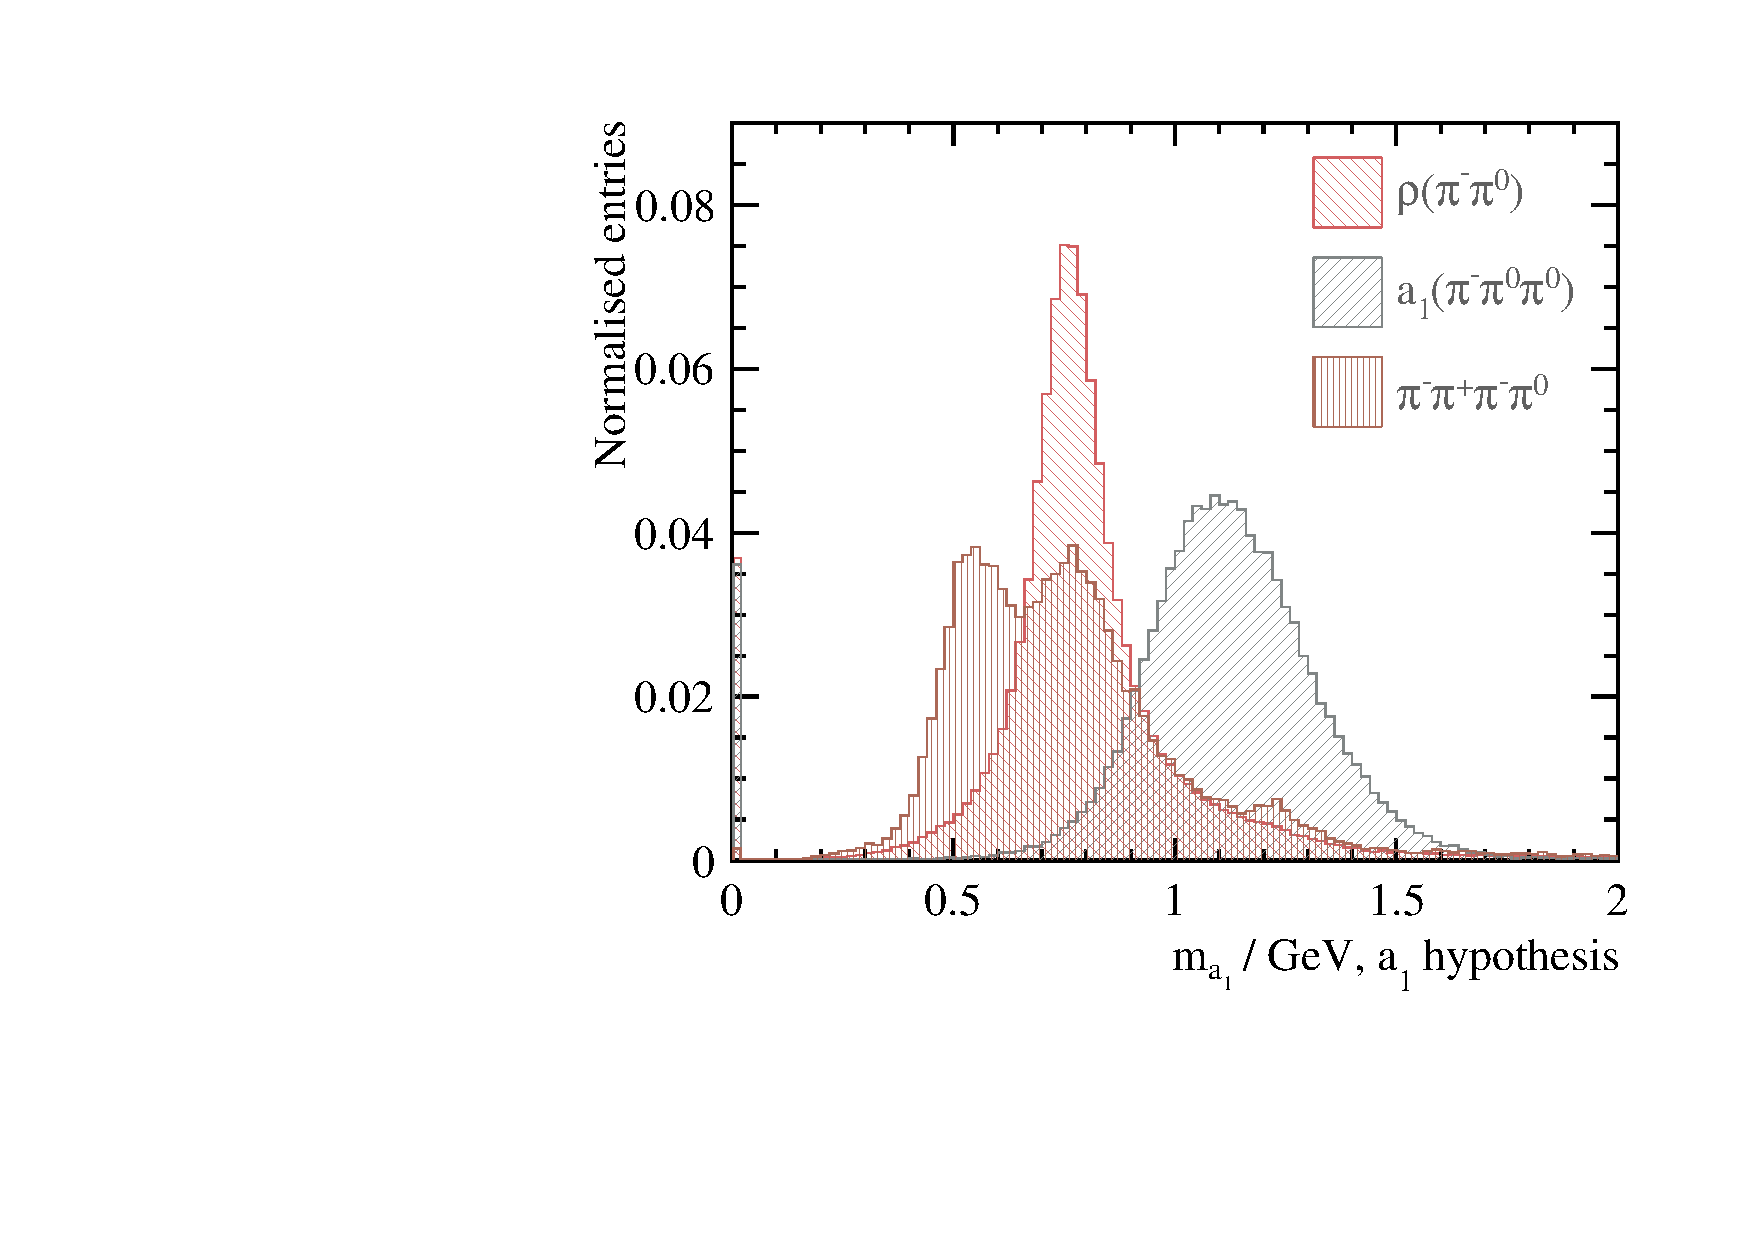
\includegraphics[width=0.65\textwidth]{tau/var3/mA1A1Fit_100GeV_improved_zoom.pdf}
\caption
{Reconstructed invariant mass distributions for \Pai ($m^{reco}_{\Pai}$), reconstructed under the  \decayAiPhotonShort decay mode hypothesis for different tau decay modes. The area under the curve is normalised to unity.}
\label{fig:tauVarMA1}
\end{figure}

\subsection{Separating electrons from charged pions}
\label{sec:tauVarEPiSeparation}
%The particle ID output by \pandora is used extensively to reconstruct variables. However, extra

Variables are used in this analysis to help further separate  electrons from charged pions, obtained from a modified private version of \pandora.

%, which could be mistaken as \Pgpm in the  reconstruction.

%In particular \pandora uses a wide range of information to determine the electron ID.

An electron develops a characteristic EM shower in the \ECAL, whilst a charged pion develops a hadronic shower. Variables characterising the  EM shower help to identify an electron. Three variables are used in the MVA classification: the start layer of the longitudinal shower ($t_0$); the fractional difference between observed and expected longitudinal EM shower profile ($\delta{l}$); and $\langle{w}\rangle$, a measure of the EM shower transverse width. These variables are defined in the same way as the variables used in the photon likelihood classifier in the photon reconstruction in \pandora, described in \Section{sec:photonLikelihood}.

The calorimeter hit information is also used to  differentiate an EM shower from a hadronic shower. Two variables used in the MVA classification are: the average energy of a calorimeter hit ($\bar{E}_{hit}$), which is the total energy deposited in the \ECAL and \HCAL divided by the number of the \ECAL and \HCAL calorimeter hits, and the average fraction of minimum ionising calorimeter hits ($MIP$), which is the number of calorimeter hits in the \ECAL and \HCAL flagged as minimum ionising particles by the \pandora reconstruction, divided by the total number of calorimeter hits in the \ECAL and \HCAL.

Finally track momentum used to provide the consistency check of the track momentum with the total energies in the \ECAL and \HCAL for charged particles. The variable used in the MVA classification is the energy in the \ECAL and \HCAL divided by the track momentum, averaged over all charged particles ($E/p$).


\FIGURE{fig:tauVar5} show distributions of the average energy of a calorimeter hit ($\bar{E}_{hit}$), and the energy in the \ECAL and \HCAL divided by the track momentum, averaged over all charged particles ($E/p$). Differences between the \decayElectron, \decayMuon, and \decayPion decay modes can be seen.
%Last information used to separate an electron  from a charged pion is the track$-$momentum calorimeter$-$energy consistency check.


%This variable is found to help to differentiate \decayElectronShort from \decayPionShort final state.


%EM shower profile & $\delta{l}$, $t_0$, $\langle{w}\rangle$ \\
%Calorimeter hit info. & $\bar{E}_{hit}$, $\%MIP$ \\
%Track info. & $\Delta E/P$ \\

\begin{figure}[htbp]
\centering
% \begin{center}/\end{center} takes some additional vertical space
\begin{subfigure}[b]{0.45\textwidth}
 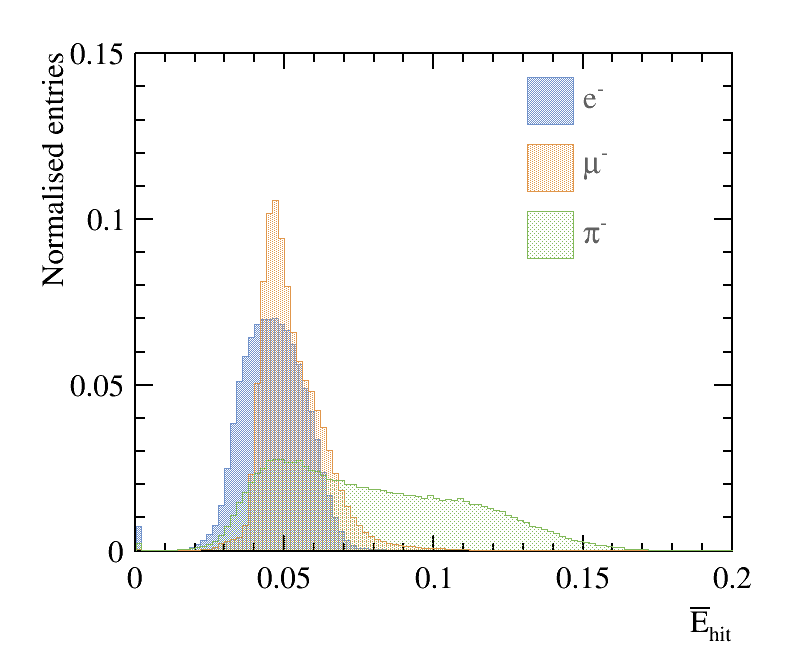
\includegraphics[width=\textwidth]{tau/var3/eCellMean_100GeV_improved}
  \caption{}
  \label{fig:tauVarECellMean}
\end{subfigure}
\begin{subfigure}[b]{0.45\textwidth}
 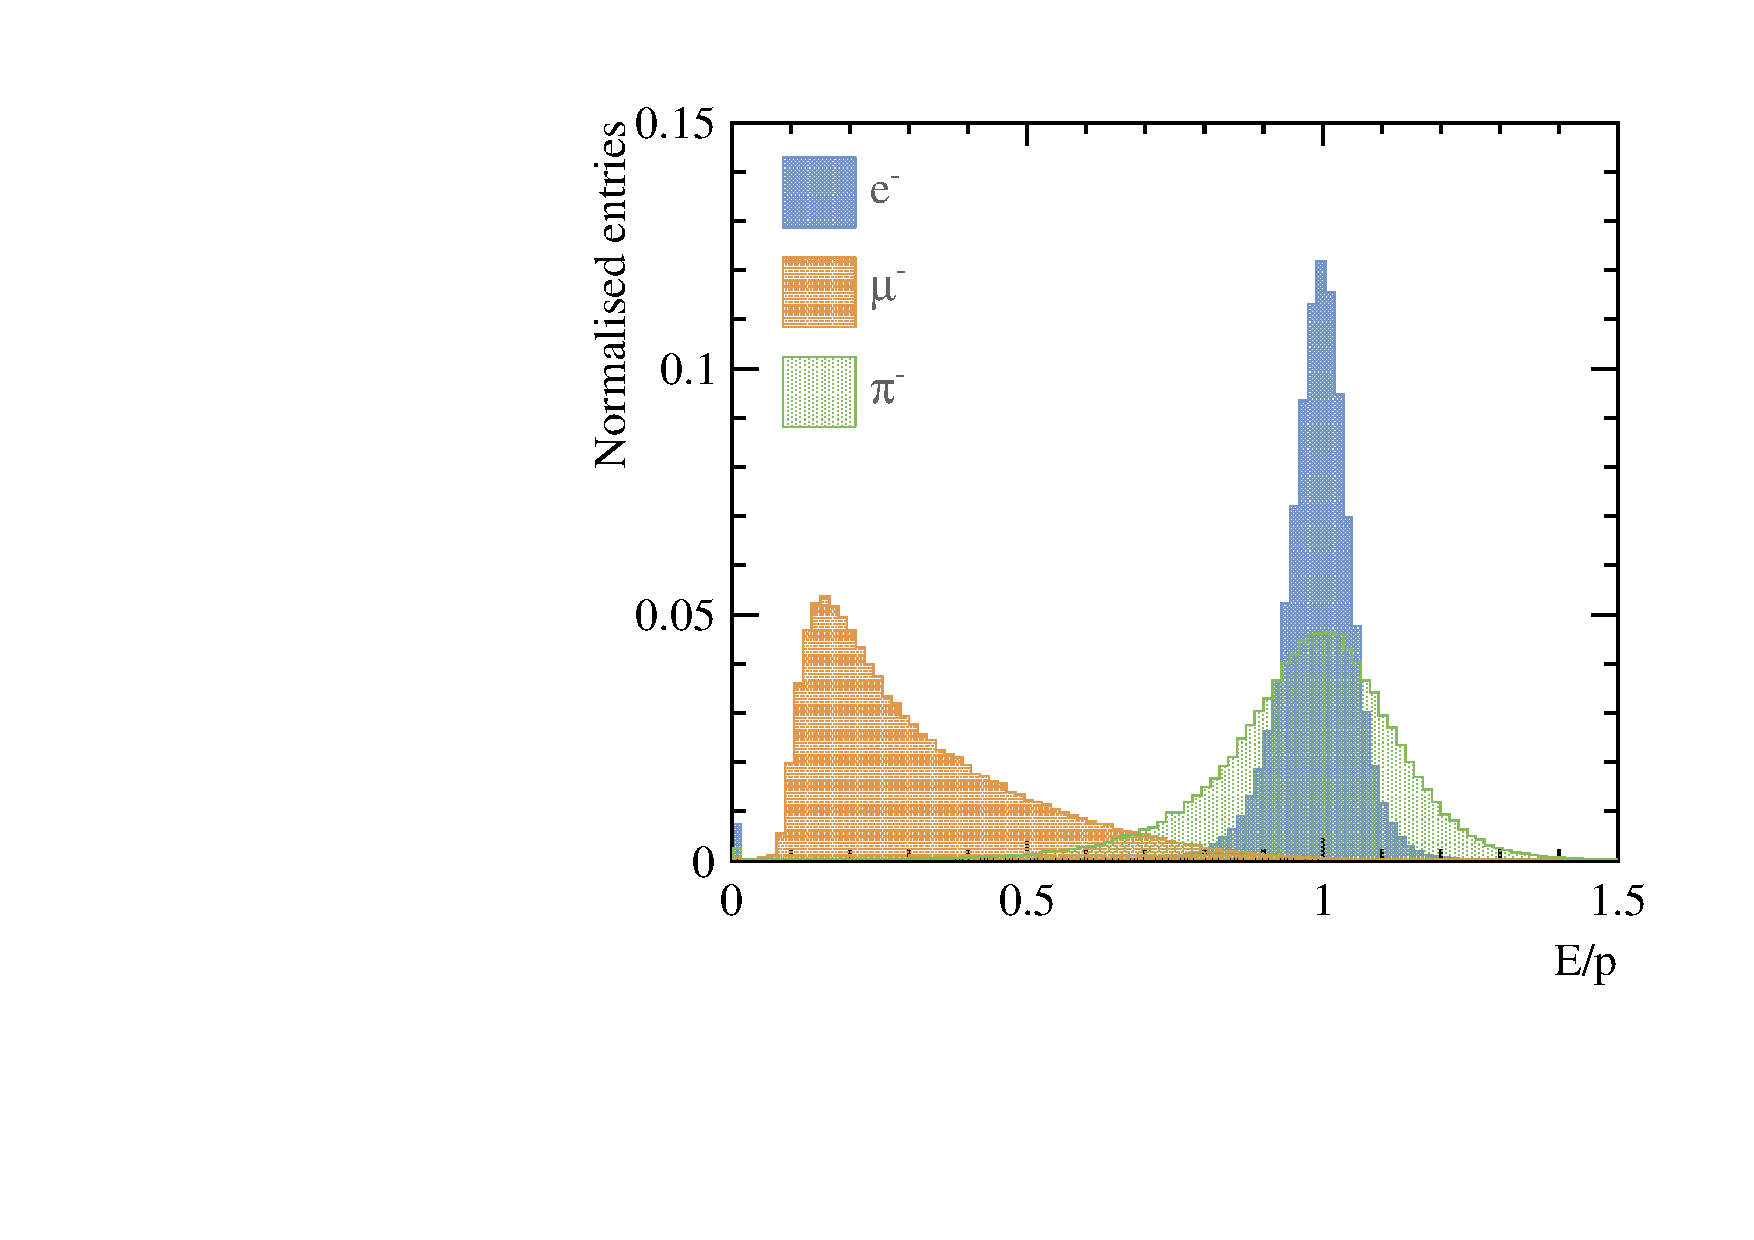
\includegraphics[width=\textwidth]{tau/var3/eOverPCharge_100GeV_improved}
  \caption{}
  \label{fig:tauVarEOverPCharge}
\end{subfigure}
\caption
{Distributions of: a) the average energy of a calorimeter hit ($\bar{E}_{hit}$); and b)  the energy in the \ECAL and \HCAL divided by the track momentum, averaged over all charged particles ($E/p$).  The area under the curve is normalised to unity.}
\label{fig:tauVar5}
\end{figure}


\section{Classification}
\label{sec:tauMVA}

The \multiclass class of the \TMVA package \cite{Therhaag:2009dp} was used to perform a multiple-class classification, which classifies seven tau lepton decay final states simultaneously. The \multiclass classification is an extension of a standard two-class signal-background classification. The Boosted Decision Tree classifier with Gradient boost (BDTG) is used. Half of the events, randomly selected, were used in the training process and the other half were used for testing. The optimisation of the BDTG classifier followed the strategy outlined in \Section{sec:pandoraMVAoptimisation}. The optimised parameters for the classifier are listed in \Table{tab:tauBDTparameters}, where an explanation of the parameters can be found in \Section{sec:pandoraMVAbdtVar}.

% The discussion on multivariate analysis can be found in \Section{sec:pandoraMVA}. In particular, the \multiclass classifier is discussed in \Section{sec:pandoraMVAmulticlass}.



\begin{table}[!htbp]\centering
%\small
\begin{tabular}{lr}
\hline \hline
 Parameter &  Value \\
\hline
Depth of tree & 5 \\
Number of trees & 3000 \\
Boosting & gradient boost \\
Learning rate of the gradient boost & 0.1 \\
Metric for the optimal cuts & Gini Index \\
Bagging fraction & 0.5 \\
Number of bins per variables & 100 \\
End node output & yes/no \\
\hline \hline
\end{tabular}
\caption
{Optimised parameters for the Boosted Decision Tree with Gradient boost \multiclass classifier used for the tau decay mode classification.}
\label{tab:tauBDTparameters}
\end{table}


\section{Tau decay mode classification efficiency}
\label{sec:tauClassificationEff}

Two million \eeToTauTau events at a centre-of-mass energy of 100\,GeV were used in the tau decay modes classification. For tau decays passing pre-selection cuts, the correct classification and misidentification  efficiencies for the seven tau decay modes are shown in \Table{tab:TauSelExample}. The correct classification efficiencies  (bold numbers in \Table{tab:TauSelExample})  are defined as:
\begin{equation}
\varepsilon_i = \frac{N^{correct}_i}{N^{MC}_i},
\label{eqn:tauEff}
\end{equation}
where $N^{correct}_i$ is the number of correctly classified tau decays for decay mode $i$ and the $N^{MC}_i$ is the total number of true tau decays for decay mode $i$.
%For example, 99.8\% events of true \decayElectronShort decay mode are reconstructed correctly.



\begin{table}[htbp]
\centering
\small
\smallskip
\begin{tabular}{ l   r  r  r  r  r  r  r }
\hline
\hline
Reco$\downarrow$ Truth$\to$& \decayElectronShort & \decayMuonShort &\decayPionShort & \decayRhoShortest &\decayAiPhotonShortest &\decayAiPionShortest &\decayThreePionPhotonShort \\
\hline

{\decayElectronShort}&\textbf{99.7}\%&-&0.9\%&0.6\%&0.4\%&-&-\\
{\decayMuonShort}&-&\textbf{99.5}\%&0.6\%&-&-&-&-\\ \cline{4-6}
{\decayPionShort}&-&0.3\%& \multicolumn{1}{| r}{\textbf{94.0}\%} &0.8\%&\multicolumn{1}{r|}{-}&0.4\%&-\\
{\decayRhoShort}&-&-& \multicolumn{1}{| r}{3.4\%}&\textbf{93.6}\%&\multicolumn{1}{r|}{9.5\%}&0.6\%&2.3\%\\
{\decayAiPhotonShort}&-&-&\multicolumn{1}{| r}{-}&4.5\%&\multicolumn{1}{r|}{\textbf{89.7}\%}&-&0.6\%\\ \cline{4-8}
{\decayAiPionShort}&-&-&0.9\%&-&\multicolumn{1}{r|}{-}&\textbf{96.8}\%&\multicolumn{1}{r|}{6.4\%}\\
{\decayThreePionPhotonShort}&-&-&-&0.3\%&\multicolumn{1}{r|}{-}&2.0\%&\multicolumn{1}{r|}{\textbf{90.6}\%}\\  \cline{7-8}

\hline
\hline
\end{tabular}

\caption[Classification efficiency for tau decay modes.]
{Classification efficiencies for the seven tau decay modes considered here. Bold numbers represent the correct classification efficiencies. Boxes highlight one-prong and three-prong tau hadronic decay modes. The entries marked with ``-'' represent numbers below 0.25\%. The absolute statistical uncertainty for each entry is less than 0.25\%.}
\label{tab:TauSelExample}
\end{table}

The particle ID from the \pandora reconstruction is effective, resulting in the correct classification efficiencies for \tauToElectron and \tauToMuon decays being 99.8\% and 99.5\% respectively. For the \tauToPion decays, only 0.9\% of decays are misclassified as \tauToElectron decays, due to the additional variables (\Section{sec:tauVarEPiSeparation}) dedicated to the separation between \Pem and \Ppiminus.

For the separation of tau hadronic decay modes, photon reconstruction is important as the number of photons is an essential variable to distinguish different hadronic decay modes. Failure to reconstruct photons in the \tauToAiPhoton decays or extra reconstructed photons in the \tauToRho decays leads to the misclassification between the \tauToAiPhoton and \tauToRho decays. Similarly, failure to reconstruct photons in the \tauToRho decays or extra reconstructed photons in the \tauToPion decays can lead to the misclassification between the \tauToRho and \tauToPion decays. The misclassification between one-prong decays, as well as between three-prong decays, is highlighted in \Table{tab:TauSelExample}.

A high correct classification rate is achieved for all seven classified tau decay modes. The leptonic decay modes have correct classification rates over 99.5\%. For the hadronic tau decay modes, classification rates of 89.7\% or above are achieved.

%For the \decayElectronShort decay mode,   99.8\%  correct classification efficiency is achieved. For the \decayMuonShort decay mode,  99.5\% correct classification efficiency is achieved.

% due to an effective track reconstruction and muon reconstruction algorithms in \pandora.

%For the \decayPionShort decay mode, 3.4\% events are misclassified as \decayRhoShortest decay mode events. If the reconstruction is unable to reconstruct two photons from \Ppizero decay in \decayRhoShortest decay mode, the \decayPionShort and \decayRhoShortest decay modes events would appear to be similar and misclassification occurs. On the other hand, only 0.9\% of \decayPionShort decay events are misclassified as \decayElectronShort decay, due to variables dedicated to separation between \Pem and \Ppiminus.

%The confusion with \decayElectronShort is at percent level, which is low due to the usage of EM shower variables. The percent level confusion with \decayAiPionShortest is because the tracking efficiency is at 98\%, where 2\% \decayPionShort events have more than one track reconstructed.

%confusion with \decayRhoShortest decay mode  is to due to differentiate two event topologies. Around 15\% of \decayPionShort events have at least one photon reconstructed, mostly due to the FSR.

%For the \decayRhoShortest decay mode, most misclassification comes from the confusion with \decayAiPhotonShortest decay mode.  If the reconstruction is unable to resolve the all photons from \Ppizero decay in \decayRhoShortest and \decayAiPhotonShortest decay mode, the two decay modes would have similar topologies.

%For the \decayAiPhotonShortest decay mode, the correct classification rate is the lowest among seven decay modes, as the final state of the \decayAiPhotonShortest decay mode is the most challenging to reconstruct correctly with four photons in the final state. The 9.5\% confusion with \decayRhoShortest decay mode is due to the same photon reconstruction failure issue. It should be noted that the distribution of the number of photons in \Figure{fig:tauVarNPhoton} suggests that 30\% of \decayAiPhotonShortest events have fewer than four photons reconstructed, overlapping with the distribution for \decayRhoShortest decay mode. The \decayAiPhotonShortest resonance reconstruction and the use of the MVA \multiclass classifier reduce the confusion between two decay modes from 30\% to  9.5\%.

%For the \decayAiPionShortest decay mode, the biggest source of misclassification is with \decayThreePionPhotonShort decay mode. The biggest misclassification of  \decayThreePionPhotonShort decay mode  is with \decayAiPionShortest decay mode.

%And the reason is the same for

%The unprecedented high classification rate has been achieved. The improvement of photon reconstruction described in \Section{} improved the ability to separate 1-prong final state. Most notably,  \Figure{} shows number of photons have a high correct reconstruction efficiency.






\section{Electromagnetic calorimeter optimisation}
\label{sec:tauECAL}

Photon reconstruction in a highly granular \ECAL is an important  metric for the \ECAL performance. Since the classification of the tau hadronic decay modes depends on the ability to reconstruct photons, tau hadronic decay modes classification is used as a metric to optimise the \ECAL design. The tau decay mode classification was studied with \ECAL square cell sizes of 3, 5, 7, 10, 15 and 20\,mm, and at four  centre-of-mass energies of 100, 200, 500, 1000\,GeV. The other \ECAL dimensions are kept the same as for  the \ILD nominal detector. The multivariate classifier was trained  individually for each \ECAL cell size and each centre-of-mass energy.


%The analysis is repeated with varying \ECAL square cell sizes at 3, 5, 7, 10, 15 and 20\,mm, at four  \sqrtS = 100, 200, 500, 1000\,GeV.
%In above sections, an analysis on tau decay mode classification is presented. Events used in the analysis were \eeToTauTau events at \rootSGeV{100} with the nominal \ILD detector model. In this section, the analysis

\pandora was optimised for the nominal \ILD detector. Therefore a re-optimisation is required for detector models with different \ECAL cell sizes. In particular, the parameters used in \PhotonFragmentRemoval algorithm need to be optimised for  different \ECAL cell sizes. The optimal \ClosestHitDistance parameter in \PhotonFragmentRemoval algorithm, which is a distance metric controlling the merging of the fragment, was chosen by selecting the value that gives the highest overall tau hadronic decay classification rate, \tauHad using \eeTauTau samples at a centre-of-mass energy of 100\,GeV.  \ClosestHitDistance is varied amongst values of 5, 10, 20, 30, 40, and 50\,mm. The overall tau hadronic decay correct classification rate, \tauHad, is the weighted average correct classification efficiency, defined as:
\begin{equation}
\tauHad = \frac{\sum_{i}^5 {B}_{i}\varepsilon_{i}}{\sum_{i}^5 {B}_{i}}  \,,
\label{eq:had}
\end{equation}
where $B_{i}$ is the branching fraction of the tau  hadronic decay mode $i$; $\varepsilon_{i}$ is the correct classification efficiency of tau decay mode $i$ (defined in \Equation{eqn:tauEff}); and the index $i$ is summed over five tau hadronic decay modes considered here:\tauToPion; \tauToRho; \tauToAiPhoton; \tauToAiPion; and \tauToThreePion.


 \TABLE{tab:TauPhotonFragmentRemovalParameter} shows the optimised values of \ClosestHitDistance parameter in  \PhotonFragmentRemoval algorithm as a function of the \ECAL square cell sizes. As expected, for larger cell sizes,  the distance metric for merging photons becomes larger.


\begin{table}[htbp]
\centering
%\small
%\smallskip
\begin{tabular}{ l   r  r  r  r  r  r  }
\hline
\hline
\ECAL square cell size /\,mm & 3 & 5 & 7 & 10 & 15 & 20  \\
\hline
\ClosestHitDistance /\,mm& 5 & 10 & 10 & 10 & 20 & 20 \\
\hline
\hline
\end{tabular}

\caption
{Optimised values of \ClosestHitDistance parameters in \PhotonFragmentRemoval algorithm as a function of the \ECAL square cell sizes.}
\label{tab:TauPhotonFragmentRemovalParameter}
\end{table}




%\tauHad  decreases with the increasing centre-of-mass energies and the increasing \ECAL cell sizes, because it is increasingly difficult to reconstruct boosted photons with lower \ECAL transverse spatial resolutions.

\FIGURE{fig:TauHadronicEfficiency} shows \tauHad as a function of \ECAL cell size for four different centre-of-mass energies. The efficiency \tauHad decreases with an increase of the centre-of-mass energy. As the centre-of-mass energy increases, the tau decay products become more boosted, making it increasingly difficult to separate tau decay products, for example, the photon pair from \Ppizero decay. The reduction in the ability to separate photon pairs leads to a degradation of  the classification performance.
% becomes very challenging to separate at a high centre-of-mass energy.

 The efficiency \tauHad decreases with the  increasing \ECAL cell sizes. The change in the \ECAL cell size will change the \ECAL transverse spatial resolution. Hence a large cell size will result in a low transverse spatial resolution, leading to a reduction in the ability to separate a pair of photons. Consequently, a worse classification performance is expected for a larger \ECAL cell size.


\begin{figure}[htbp]
\centering % \begin{center}/\end{center} takes some additional vertical space
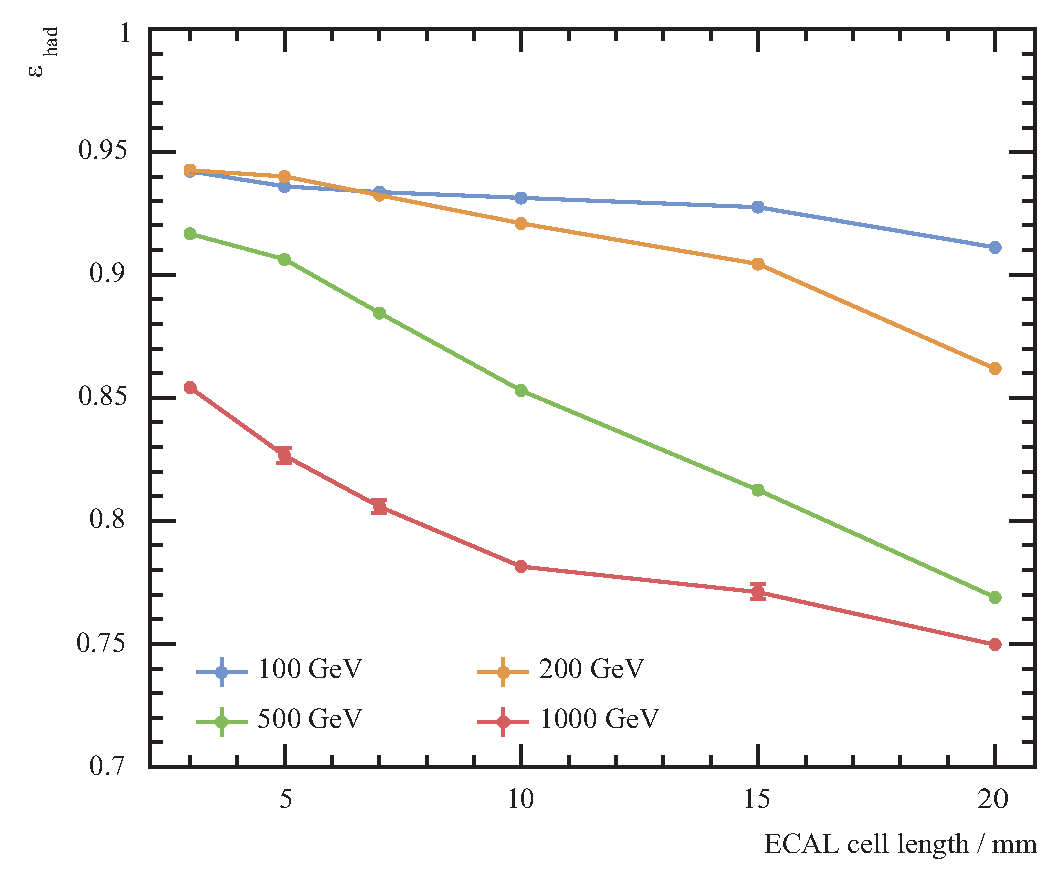
\includegraphics[width=.85\textwidth]{tau/plots3/hadronicEff2}
\caption[The tau hadronic decay efficiency as a function of  the \ECAL cell sizes at different \sqrtS with the \ILD detector model.]
{The weighted average tau hadronic decay correct classification efficiency, \tauHad, as a function of  the \ECAL cell sizes for four different centre-of-mass energies. The blue, orange, green, and red points  show \tauHad at \sqrtS = 100, 200, 500, and 1000\,GeV, respectively.}
\label{fig:TauHadronicEfficiency}
\end{figure}

%\FIGURE{fig:TauPionEfficiency} shows that

%This trend is observed for almost all tau decay modes.

\TABLE{tab:TauTauHad} lists the achieved hadronic decay mode separation, as measured by \tauHad, with 3\,mm and 20\,mm \ECAL cell sizes for four different centre-of-mass energies. The sensitivity of \tauHad to different cell sizes is stronger at high centre-of-mass energies.  With decay products being spatially close at high centre-of-mass energies, it is more beneficial to have a small \ECAL cell size to reconstruct individual particles.


\begin{table}[htbp]
\centering
%\small
%\smallskip
\begin{tabular}{ l   r r }
\hline
\hline
\tauHad & 3\,mm & 20\,mm  \\
\hline
100\,GeV & 94\% & 91\% \\
200\,GeV & 94\% & 86\% \\
500\,GeV & 92\% & 78\% \\
1000\,GeV & 85\% & 75\% \\
\hline
\hline
\end{tabular}

\caption
{\tauHad with 3\,mm and 20\,mm \ECAL cell sizes for four different centre-of-mass energies.}
\label{tab:TauTauHad}
\end{table}


\FIGURE{fig:TauPionEfficiency} shows the correct classification efficiencies ($\varepsilon_{i}$) for five  tau hadronic decay modes as a function of the \ECAL square cell sizes for four different centre-of-mass energies. The tau decay mode correct classification efficiencies generally decrease with an increase of centre-of-mass energies and an increase of \ECAL cell sizes.


For the \tauToRho decay mode, the efficiency at  \rootSGeV{1000} increases as the cell size increases. This is because the multivariate classifier optimises for the overall classification efficiency, which may balance the decrease of the efficiency of one decay mode by the increase of the efficiency of another decay mode. In this case, the small increase in the efficiency for \tauToRho decay mode at \rootSGeV{1000} is compensated by the drastic decrease in the efficiency for \tauToAiPhoton decay mode at the same centre-of-mass energy. For this reason, \tauHad gives a better picture of true performance.

For the \tauToAiPhoton decay mode, the loss of efficiency with an increasing \ECAL  cell size and an increasing centre-of-mass energy is most significant comparing to other decay modes. With morephotons in the final state, it is the most challenging decay mode to reconstruct and thus most sensitive to the change in cell sizes and centre-of-mass energies.

For the \tauToAiPion decay mode, the efficiencies are similar to that of the \tauToPion decay mode. Both final states contain charged particles only. Therefore it is most sensitive to the tracking detector performance, which is not affected by different \ECAL cell sizes.


\begin{figure}[htbp]
\centering % \begin{center}/\end{center} takes some additional vertical space
\begin{subfigure}[b]{0.45\textwidth}
  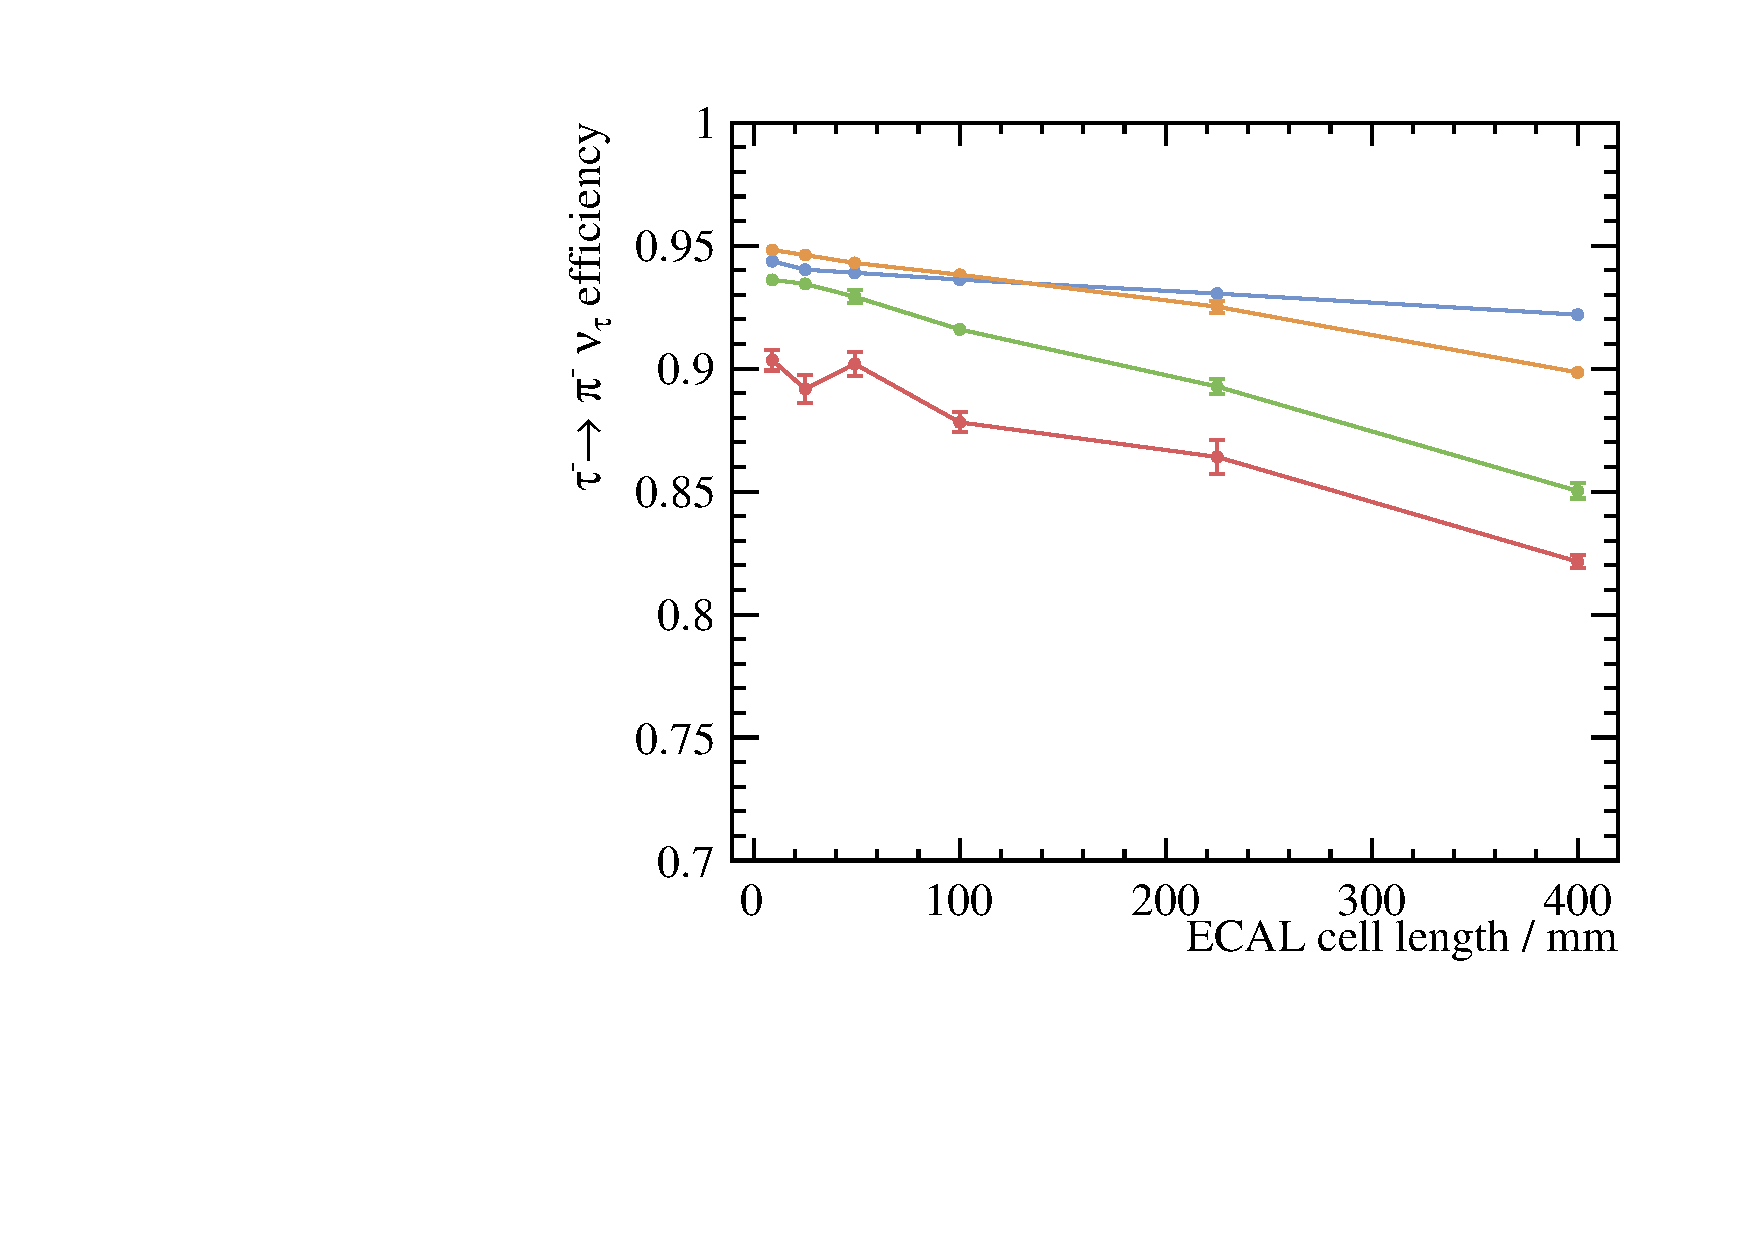
\includegraphics[width=\textwidth]{tau/plots3/decayMode2.pdf}
  \caption{}
  \label{fig:tauDecayMode2}
\end{subfigure}
\begin{subfigure}[b]{0.45\textwidth}
  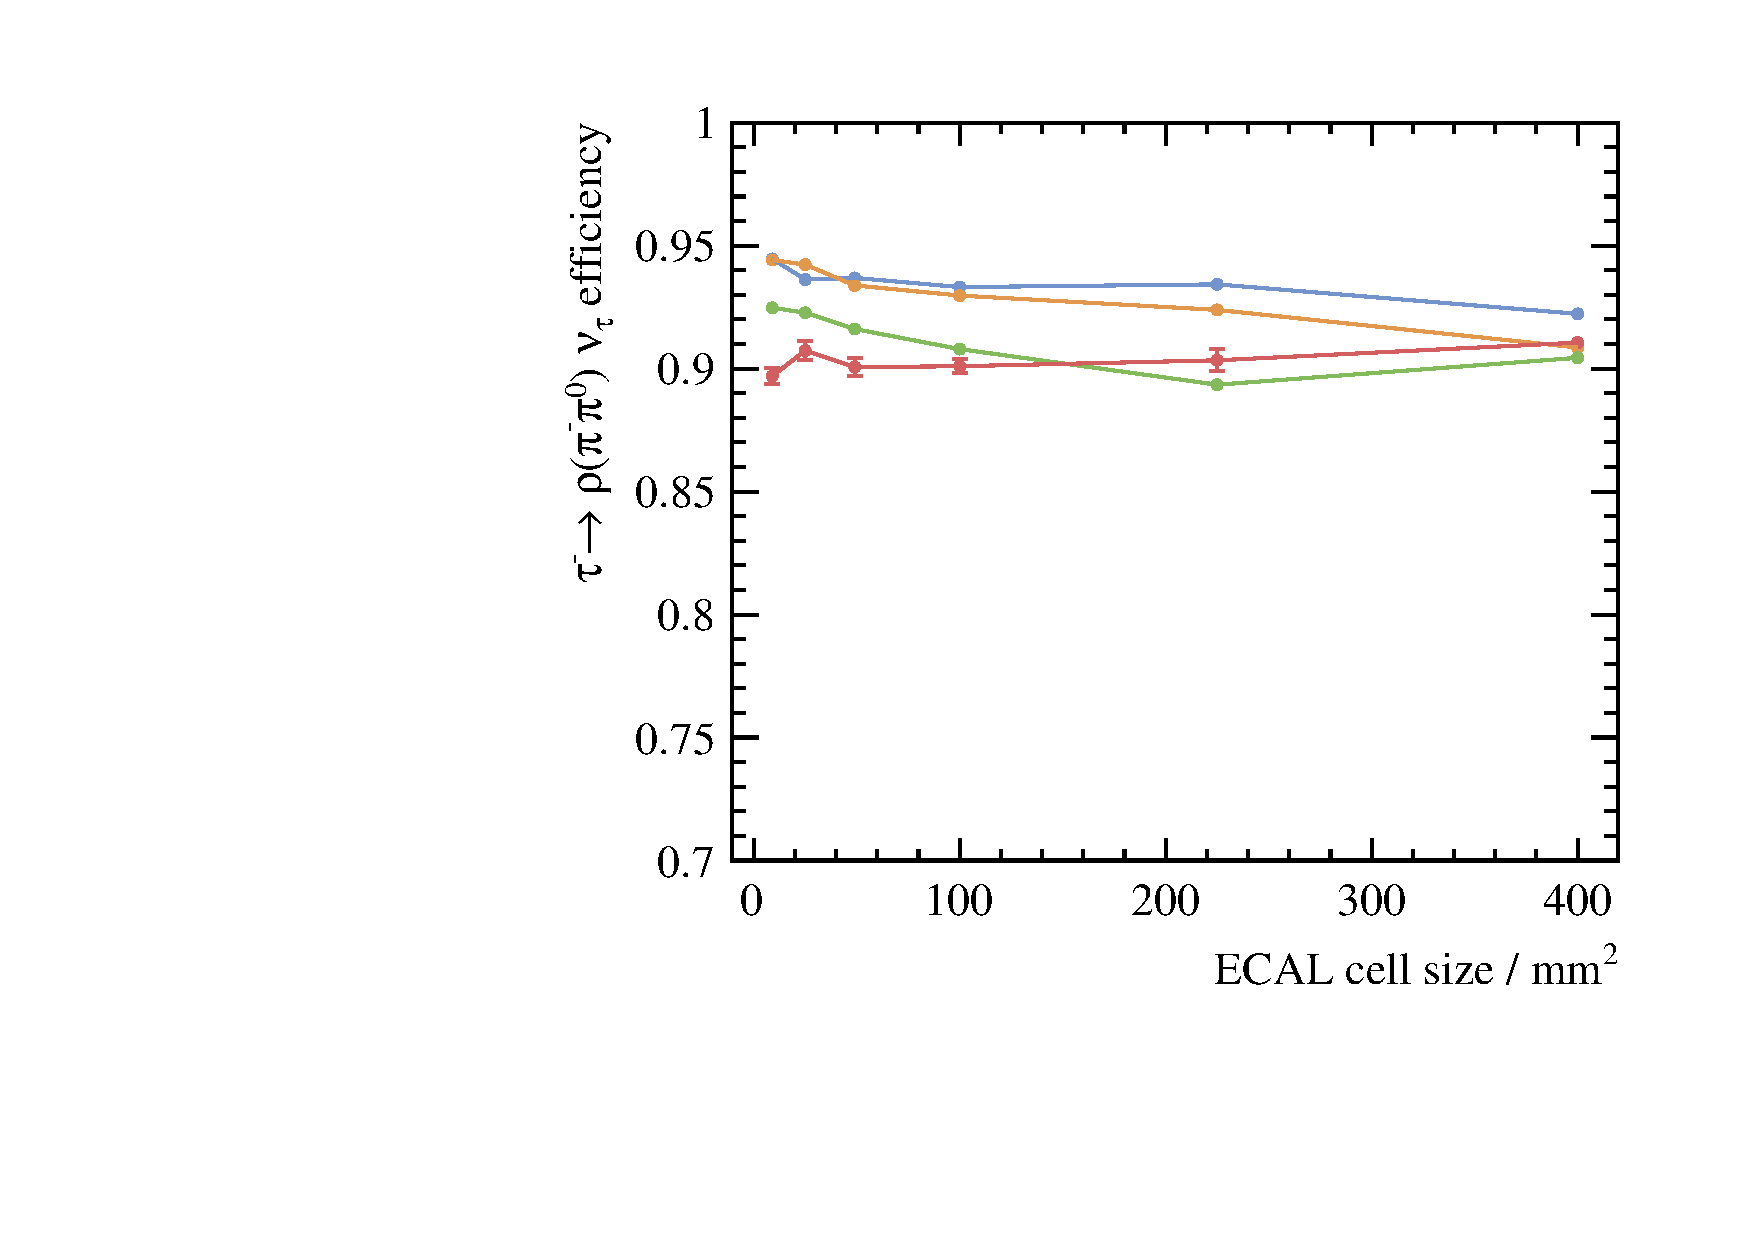
\includegraphics[width=\textwidth]{tau/plots3/decayMode3.pdf}
  \caption{}
  \label{fig:tauDecayMode3}
\end{subfigure}
\begin{subfigure}[b]{0.45\textwidth}
  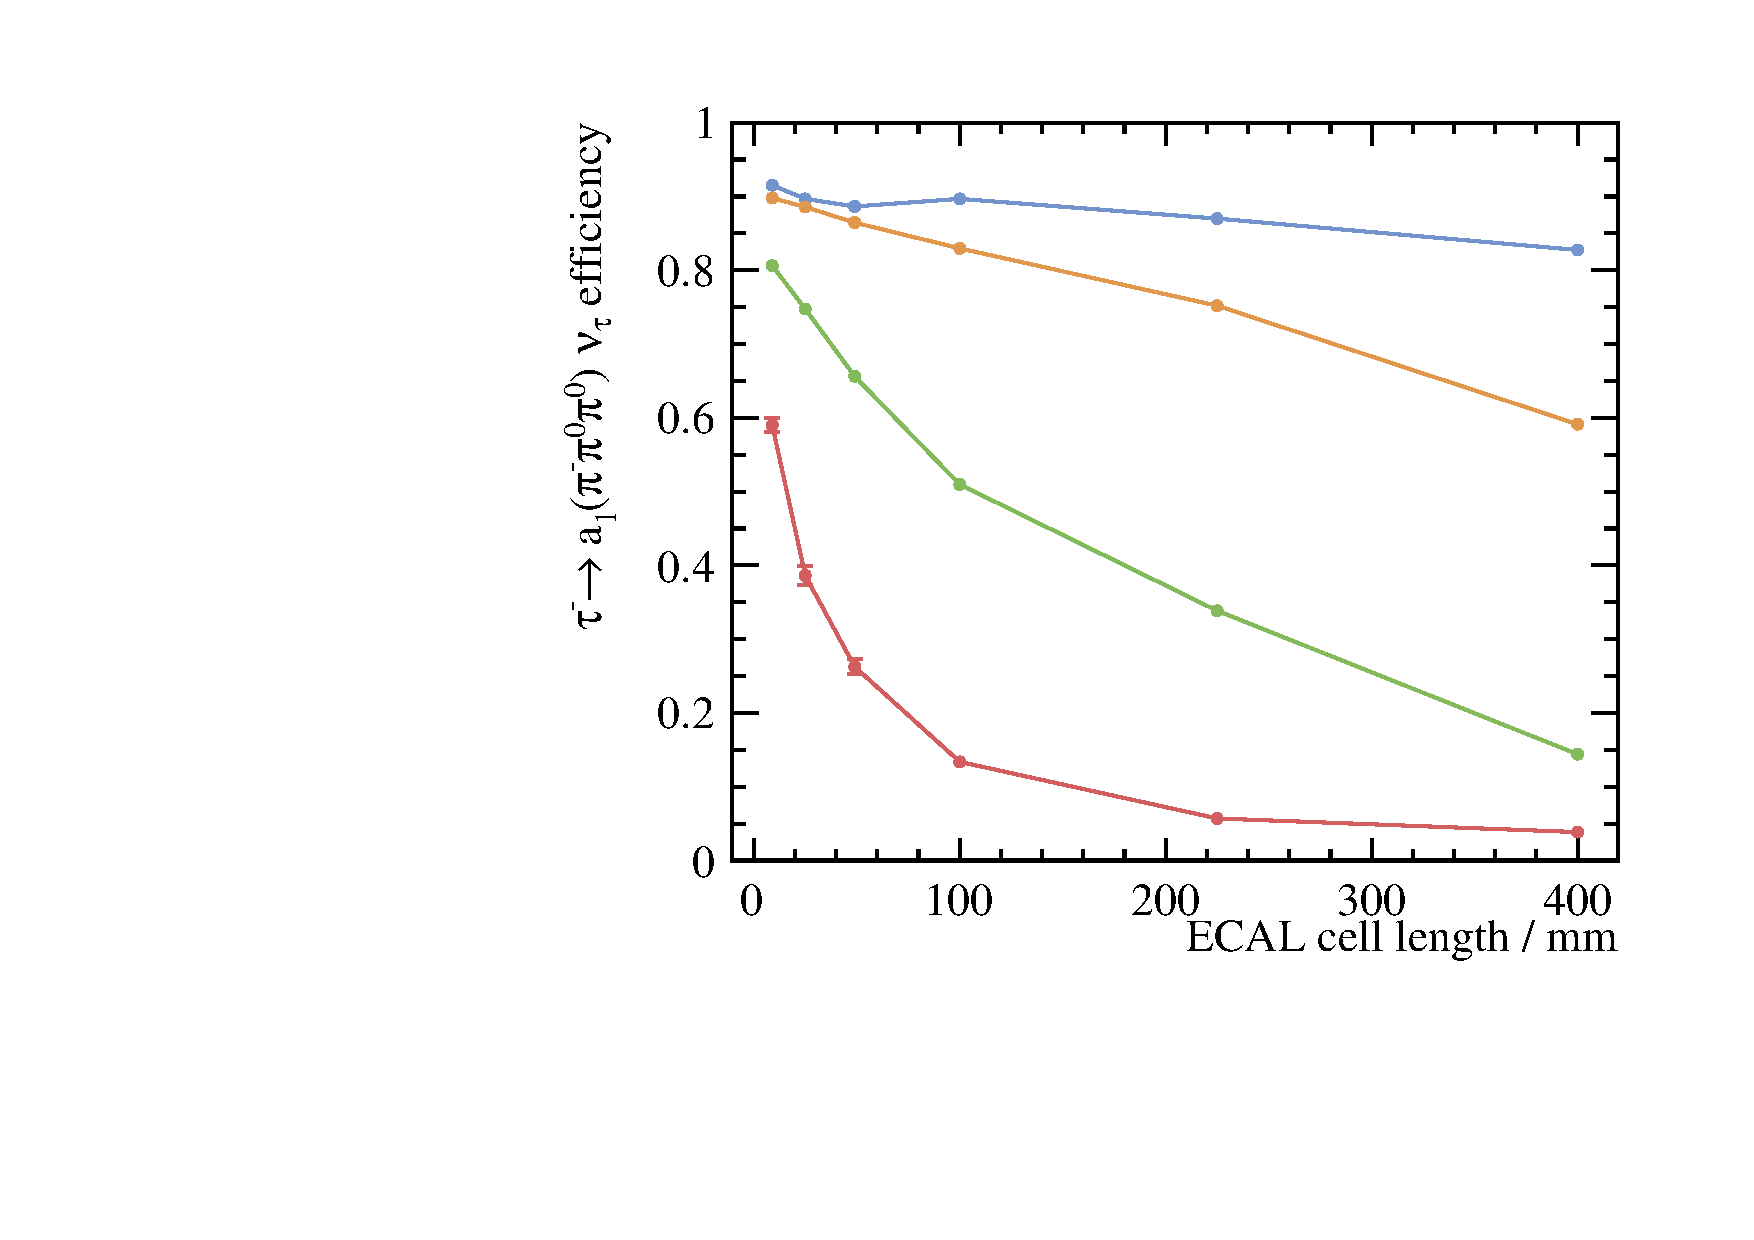
\includegraphics[width=\textwidth]{tau/plots3/decayMode4.pdf}
  \caption{}
  \label{fig:tauDecayMode4}
\end{subfigure}
\begin{subfigure}[b]{0.45\textwidth}
  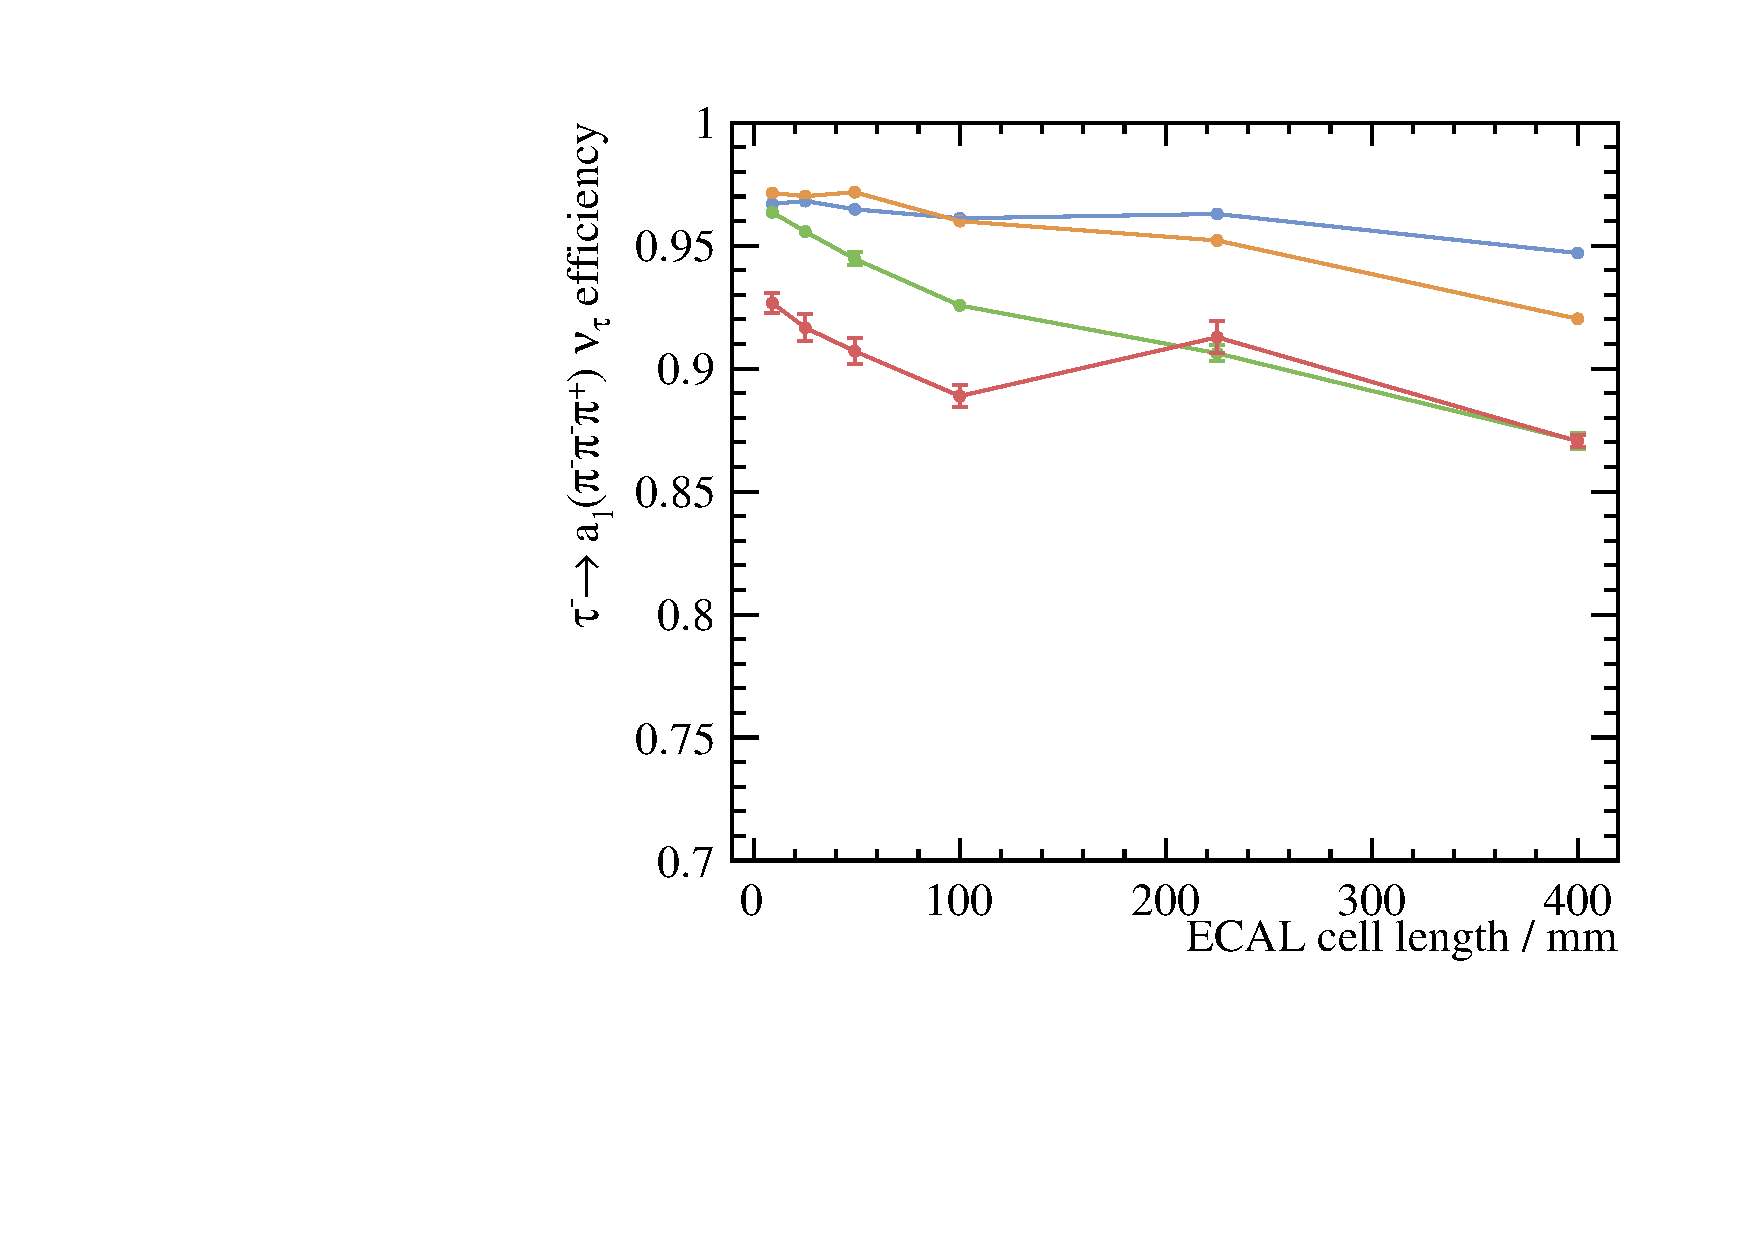
\includegraphics[width=\textwidth]{tau/plots3/decayMode5.pdf}
  \caption{}
  \label{fig:tauDecayMode5}
\end{subfigure}
\begin{subfigure}[b]{0.45\textwidth}
  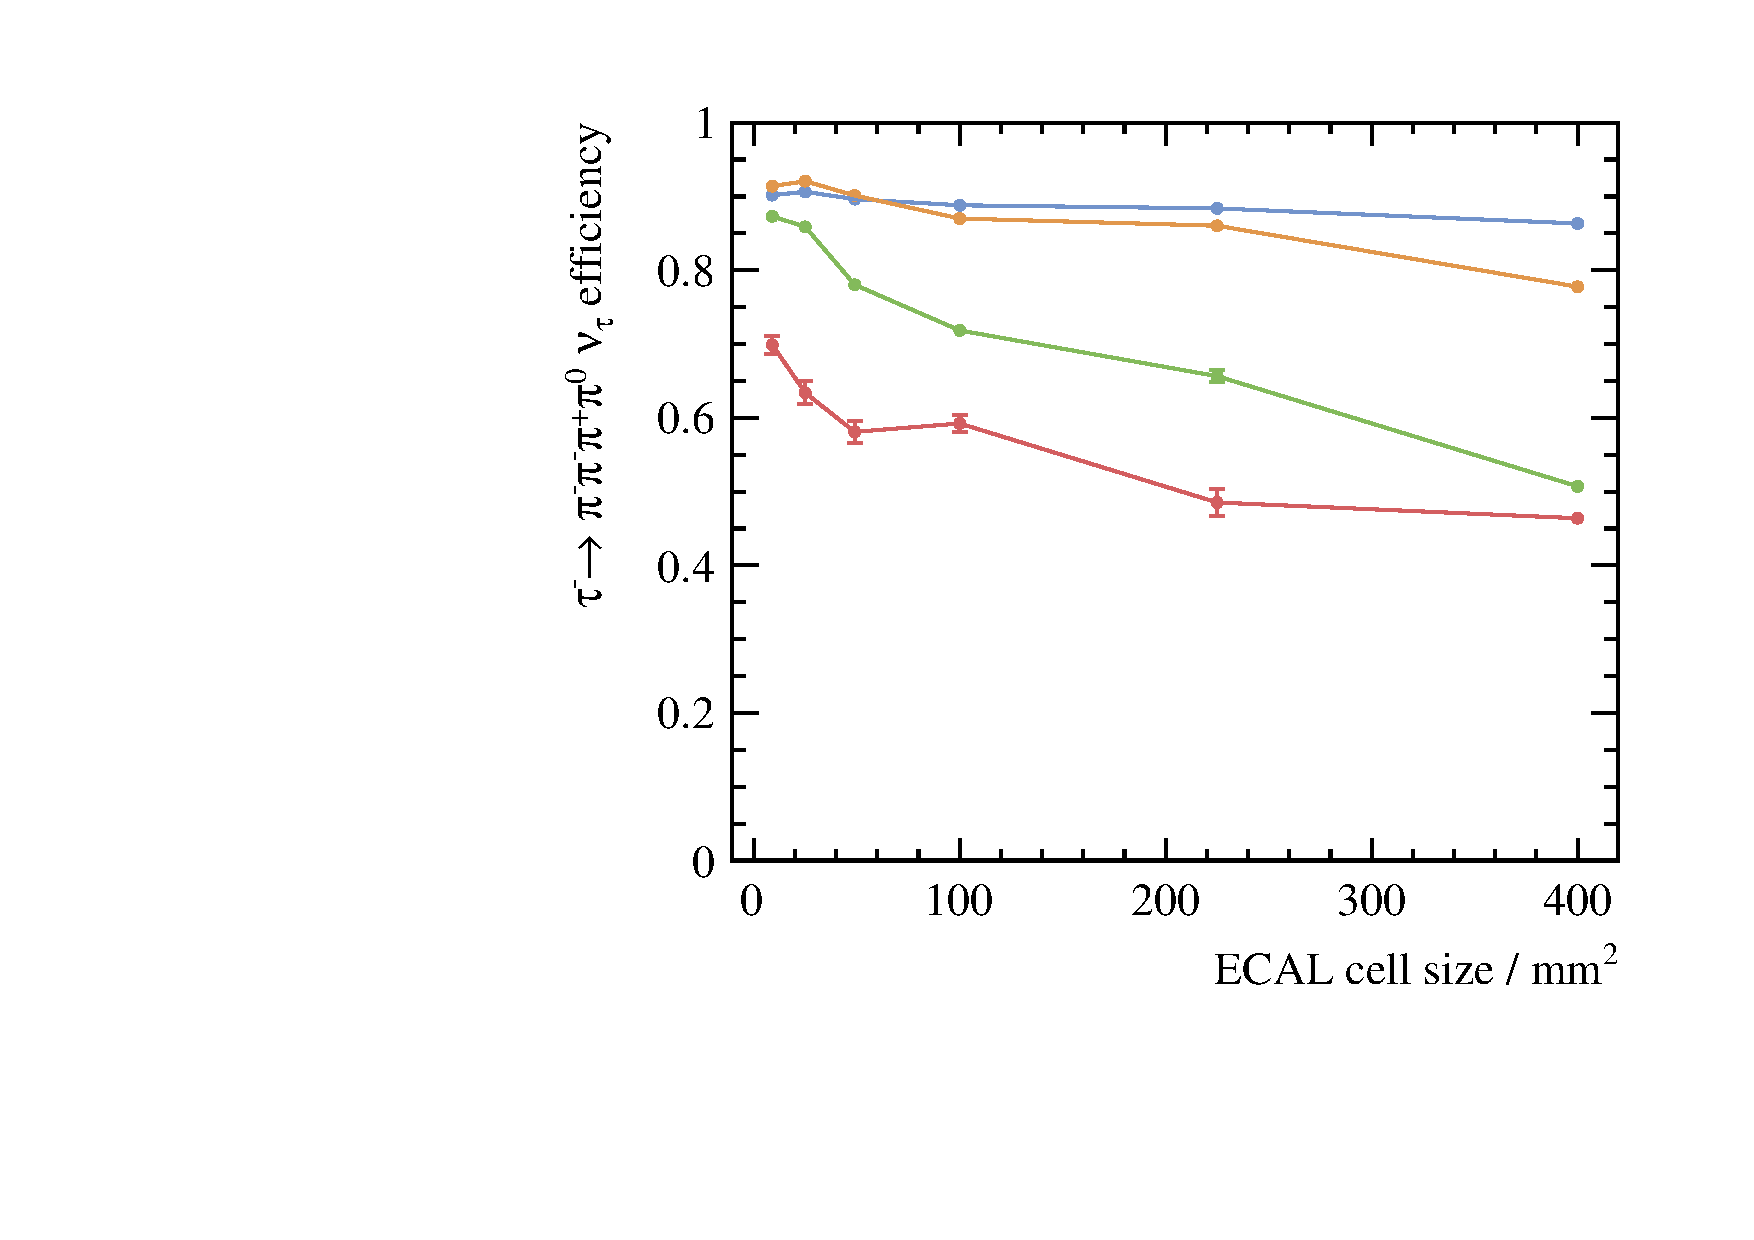
\includegraphics[width=\textwidth]{tau/plots3/decayMode6.pdf}
  \caption{}
  \label{fig:tauDecayMode6}
\end{subfigure}
\begin{subfigure}[b]{0.45\textwidth}
  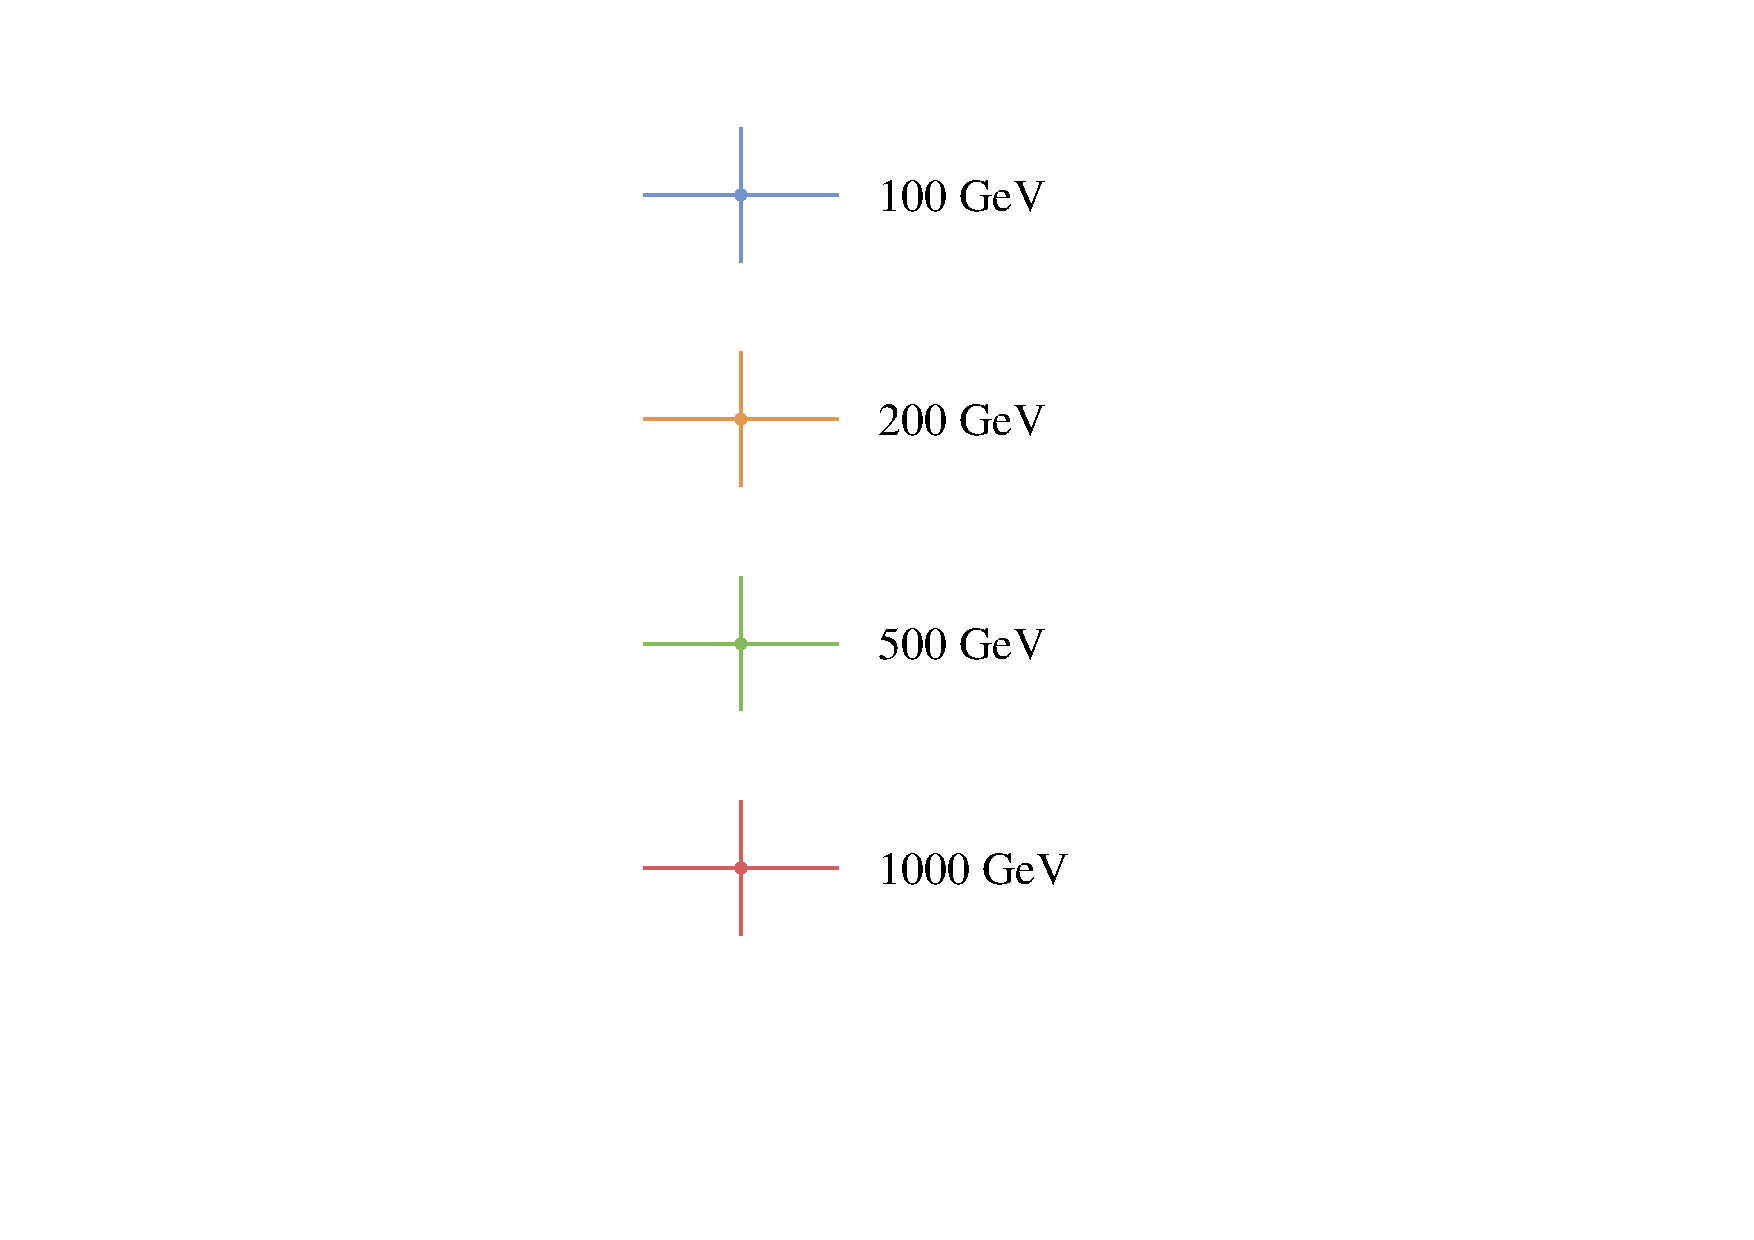
\includegraphics[width=\textwidth]{tau/plots3/legend.pdf}
  %\caption{}
  \label{fig:tauDecayLegend}
\end{subfigure}
\caption[The correct classification efficiency for  tau hadronic decay final states  as a function of the \ECAL square cell sizes]
{ The correct classification efficiencies as a function of the \ECAL square cell sizes for: a) \tauToPion decays; b) \tauToRho decays; c) \tauToAiPhoton decays; d) \tauToAiPion decays; and e) \tauToThreePion decays. Results are shown for centre-of-mass energies of 100, 200, 500, and 1000\,GeV.}
\label{fig:TauPionEfficiency}
\end{figure}



A previous study \cite{Tran:2015nxa} on the tau decay mode classification was performed using the \ILD detector on \decayPion, \decayRho, and \decayAiPhoton decay modes. Samples used were \HepProcess{\ee \to \PZz \to \TauTau(\Pphoton)} at 250\,GeV. Pre-selection required that events with photon converted to electron pairs in the tracking detector were discarded. \Garlic \cite{Reinhard:2009jh,Jeans:2012jj} photon reconstruction was used to reconstruct photons in the events. The main differences in the analyses are the pre-selection cuts, the photon reconstruction algorithm,  and the number of classified decay modes: seven versus three in previous study. \TABLE{tab:TauCompareGarlic} lists the correct classification rates  of  \decayPion, \decayRho, and \decayAiPhoton decay modes for current analysis with \pandora photon reconstruction at a centre-of-mass energies of 200\,GeV  and previous analysis using \Garlic photon reconstruction. Similar correct classification rates are achieved for \decayPion, \decayRho, and \decayAiPhoton decay modes.


\begin{table}[htbp]
\centering
%\small
%\smallskip
\begin{tabular}{ l   r r }
\hline
\hline
Decay mode & \pandora \rootSGeV{200} & \Garlic \rootSGeV{250}  \\
\hline
\decayPion & 94.6\%\pm0.1\% & 96.8\%\pm0.2\% \\
\decayRho & 94.2\%\pm0.1\% & 90.5\%\pm0.2\% \\
\decayAiPhoton & 88.6\%\pm0.2\% & 91.1\%\pm0.4\% \\
\hline
\hline
\end{tabular}

\caption
{Correct classification rates  of  \decayPion, \decayRho, and \decayAiPhoton decay modes for current analysis with \pandora photon reconstruction and previous analysis using \Garlic photon reconstruction. Values for the previous analysis are taken from \cite{Tran:2015nxa}.}
\label{tab:TauCompareGarlic}
\end{table}

\section{Summary}

For the \ILC at \rootSGeV{250} or \CLIC at \rootSGeV{350}, an \ECAL size of 10\,mm or fewer is sufficient to achieve a \tauHad of 92\%. For a linear collider operating at a centre-of-mass energy above a few hundred GeVs, such as the \ILC at \rootSGeV{500} or \CLIC at \rootS{1.4} or \rootS{3}, it is preferable to have a small \ECAL cell size, i.e. 3\,mm,  for the best tau decay mode separation, as \tauHad decreases drastically with an increasing \ECAL cell size.

\begin{comment}

Because the electron and muon reconstruction mostly rely on the performance of the tracking system, which was not varied in this study, only the   tau hadronic decay modes were investigated for the \ECAL optimisation study.
%The general trend for t
%As the \sqrtS increases, tau decay products are boosted and it is challenging to separate identical decay products. Similarly,  increasing \ECAL cell sizes makes particle separation more difficult.

At a centre-of-mass energy of 100\,GeV, the \tauHad decreases from 94\% at 3\,mm \ECAL cell size, to 91\% at 20\,mm \ECAL cell size. The decrease in \tauHad is approximately linear to the increase in the cell size. The decrease in the \tauHad is greater at a centre-of-mass energy of 200\,GeV, where the \tauHad declines from 94\% at 3\,mm cell size, to 86\% for a  cell size of  20\,mm. The most significant degradation in the \tauHad occurs at  a centre-of-mass energy of 500\,GeV, where the \tauHad decreases from 92\% at 3\,mm cell size, to 78\% at 20\,mm cell size. At a centre-of-mass energy of 1000\,GeV, the \tauHad drops from 85\% at 3\,mm cell size, to 75\% at 20\,mm cell size.

%From 10\,mm cell size onwards, the \tauHad decrease slows down.

The increase in \ECAL cell sizes has a larger impact on the performance of the tau decay classification at high centre-of-mass energies. When the cell size is increased from 3\,mm to 20\,mm, the degradation of \tauHad is greater at \rootSGeV{500} and 1000\,GeV, than the degradation  of \tauHad at \rootSGeV{100} and 200\,GeV. With decay products being spatially close at high centre-of-mass energies, it is more beneficial to have a small \ECAL cell size to reconstruct individual particles.



%For example, the \PhotonFragmentRemoval algorithm which merges photon fragments uses a distance metric that depends on the \ECAL cell sizes.


%An increase of the \ECAL cell sizes   degrading the classification performance.



%For the \decayPionShort decay mode, the general trend is followed. The efficiency for \rootSGeV{200} is slightly better than that of the \rootSGeV{100} for small cell sizes.

For the \decayRhoShort decay mode, the efficiency for  \rootSGeV{1000} increases as the cell size increases. This is because the multivariate classifier optimises for the overall classification efficiency, which may balance the decrease of the efficiency of one decay mode by the increase of the efficiency of another decay mode. In this case, the small increase in the efficiency for \decayRhoShort decay mode at \rootSGeV{1000} is compensated by the drastic decrease in the efficiency for \decayAiPhotonShort decay mode at the same centre-of-mass energy.

For the \decayAiPhotonShort decay mode, the loss of efficiency with an increasing \ECAL  cell size and an increasing centre-of-mass energy is most significant comparing to other decay modes. With most number of photons in the final state, it is the most challenging decay channel to reconstruct and thus most sensitive to the change in cell sizes and centre-of-mass energies.

For the \decayAiPionShort decay mode, the efficiencies are similar to that of the \decayPionShort decay mode. Both final states contain charged particles only. Therefore it is most sensitive to the tracking performance, which is not affected by the  varying of the \ECAL cell sizes.
\end{comment}
%For the \decayThreePionPhotonShort decay mode, the decreases in efficiencies are more significant for \rootSGeV{500} and 1000\,GeV.

%The   correct reconstruction efficiency of the tau leptonic decay is not used as a metric as they are similar across different \ECAL cell sizes. This is because the \Pepm and \Pgmpm identifications mostly rely on the tracking system, which was not varied in this study. However the energy deposited in the calorimeter are also used for the association to the tracks. But the calorimeters have a small impact on the electron and  muon identification.

%This classification can be applied for different  \sqrtS and with different detector models. The main reconstruction issue is to separate boosted photon pair from \Ppizero decay. High \sqrtS The \ECAL cell size is crucial in separating the EM showers from photons. As discussed in previous chapter, separating photons requires a high transverse spatial resolution. Therefore, the \ECAL square cell size is expected to affect the classification efficiency.

%The main difficulty in the classification is to classify 1-prong final states.  These final states involves \Ppizero, where two photons from \Ppizero decay could be poorly reconstructed. At high energy, \Ppizero is boosted making the reconstruction more challenging. The ability to reconstruct the two photons as separate entities requires good pattern recognition algorithm for photons and \ECAL spatial resolution. Hence the improved photon reconstruction in \Chapter{chap:Photon} is used in this study. The impact of the \ECAL transverse spatial resolution on the tau decay classification is demonstrated as well.





%\FIGURE{fig:TauPionEfficiency} shows the correct classification efficiencies for  tau hadronic decay final states  as a function of the \ECAL square cell sizes. For example, plotted values for 5\,mm cell size at \rootSGeV{100} are the same as the bold numbers in \Table{tab:TauSelExample}.



%\subsection{Tau hadronic decay correct classification efficiency}
